\documentclass[a4paper,12pt]{article}
% -------------------------------------------------------------------
%                  Essential packages (used in template)
% -------------------------------------------------------------------

\usepackage[utf8]{inputenc}                   % Allow Umlauts (ä, ö, ü)
\usepackage[english, ngerman]{babel, translator}       % German LaTeX-intern descriptors (Abbildungen, ...)
\usepackage{mathptmx}                         % Font "Times New Roman" in mathematical Environments
\usepackage{courier}                          % Support the use of font "Courier" (used in listings)
\usepackage[T1]{fontenc}                      % Change LaTeX font encoding to support modern fonts
\usepackage{fix-cm}                           % Fix sizes at which CM and EC fonts can be used

\usepackage{geometry}                         % Change text bounds on a per-page basis
\usepackage{fancyhdr}                         % Allow easy customization of headers and footers

\usepackage[ddmmyyyy]{datetime}               % Reformat times from LaTeX commands like \today

\usepackage[usenames,dvipsnames]{xcolor}      % Support text colorization

\usepackage{colortbl}                         % Support applying colors to tables
\usepackage{array}                            % Tables with fixed column size
\usepackage{longtable}                        % Support multi-page tables
\usepackage{multicol}                         % Additional settings for \multicolumn
\usepackage{multirow}                         % Additional settings for \multirow

\usepackage[hyphens,obeyspaces,spaces]{url}   % Allow urls to have line breaks at "-"
\usepackage{hyperref}                         % Clickable hyperlinks in Table of Contents
\usepackage{microtype}                        % Enable "Blocksatz"

\usepackage{float}                            % Support for table H option
\usepackage{floatflt}                         % Support text wrapping around floating environments
\usepackage{wrapfig}                          % Support text wrapping around figures

\usepackage{graphicx}                         % Support including graphics environments for images
\usepackage{caption}                          % Provide greater customization around captions
\usepackage{subcaption}                       % Caption support for subfigures

\usepackage[onehalfspacing]{setspace}         % Set line spacing to be 1.5x the default
\usepackage{listings}                         % Code block support for LaTeX

\usepackage[titles]{tocloft}                  % More options to modify list of figures & tables
\usepackage{nomencl}                          % Support for nomenclatures ("Symbolverzeichnis")

\usepackage{amsmath}                          % Includes a plethora of mathematical packages 
\usepackage{amssymb}                          % Source mathematical symbols like \sin
\usepackage{amsthm}                           % Better theorems
\usepackage{upgreek}                          % Use \Upomega to get a straight \Omega
\usepackage{siunitx}                          % Unified support for si units

\usepackage{ifthen}                           % Support better if statements in LaTeX
\usepackage{etoolbox}                         % Easily patch commands

\usepackage{booktabs}

% Support list of acronyms and glossary
\usepackage[
  toc,
  nogroupskip,
  nonumberlist,
  nopostdot,
  acronyms,
  shortcuts,
  translate=babel
]{glossaries}

% Code color
\definecolor{dkgreen}{rgb}{0,0.6,0}
\definecolor{gray}{rgb}{0.5,0.5,0.5}
\definecolor{mauve}{rgb}{0.58,0,0.82}

\lstset{frame=tb,
  language=C++,
  aboveskip=3mm,
  belowskip=3mm,
  showstringspaces=false,
  columns=flexible,
  basicstyle={\small\ttfamily},
  numbers=none,
  numberstyle=\tiny\color{gray},
  keywordstyle=\color{blue},
  commentstyle=\color{dkgreen},
  stringstyle=\color{mauve},
  breaklines=true,
  breakatwhitespace=true,
  tabsize=3
}

% Track the total count of different environments
% Needs to be imported because LaTeX resets these counter on a chapter basis
\usepackage[figure,table,lstlisting,xspace]{totalcount}

% Annotate different information directly into the document
\setlength{\marginparwidth}{2cm}
\usepackage[
  colorinlistoftodos,
  prependcaption,
  textsize=tiny
]{todonotes}

% -------------------------------------------------------------------
%                 Useful packages (not used in template)
% -------------------------------------------------------------------

\usepackage{pdfpages}                         % Include existing PDFs into the work

% Create electrical diagrams within LaTeX
\usepackage[
  european,
  oldvoltagedirection,
  straightvoltages,
  siunitx
]{circuitikz}
% Disable single lines at the start of a paragraph (Schusterjungen)
\clubpenalty=10000

% Disable single lines at the end of a paragraph (Hurenkinder)
\widowpenalty=10000
\displaywidowpenalty=10000

% Fixed size table columns
\newcolumntype{L}[1]{>{\raggedright\arraybackslash}p{#1}}
\newcolumntype{C}[1]{>{\centering\arraybackslash}p{#1}}
\newcolumntype{R}[1]{>{\raggedleft\arraybackslash}p{#1}}

\renewcommand{\arraystretch}{1.2}                       % Distance between lines in tables

\captionsetup{justification=raggedright}                % Align captions to the left

\setcounter{secnumdepth}{3}                             % Only allow nesting 3 layers (down to subsubsections)

% Unit-related setup for siunitx
\sisetup{
  locale=DE,                   % Use German notation (comma instead of point delimiter for floats)
  per-mode=fraction,           % Switch display to use \frac instead of x^{-1}
  fraction-function=\tfrac,    % Use amsmath's tfrac macro for unit fractions
}

% -------------------------------------------------------------------
%                     Usability & visual changes
% -------------------------------------------------------------------

% Page margins
\geometry{
  left=2.5cm,
  right=2.5cm,
  top=2.5cm,
  bottom=3cm
}

% Create a better looking header and footer
\pagestyle{fancy}
\fancyhf{}
\lhead{\nouppercase{\leftmark}}
\rfoot{\thepage}

% Automatically generate a box around figure environments
\floatstyle{boxed}
\restylefloat{figure}

% Set toc sections to be clickable
\hypersetup{
  colorlinks,
  citecolor=black,
  filecolor=black,
  linkcolor=black
}

\frenchspacing                                          % Insert one space after a sentence, not 2

\renewcommand{\UrlFont}{\color{blue}\rmfamily\itshape}  % URLs should be displayed in blue
\renewcommand{\dateseparator}{.}                        % Dates are written like 01.01.1970, not 01-01-1970

\addto{\captionsngerman}{
  \renewcommand*{\figurename}{Abb.}                     % Figures should be displayed as "Abb. x"
  \renewcommand*{\tablename}{Tab.}                      % Tables  should be displayed as "Tab. x"
  \renewcommand*{\lstlistingname}{Code}                 % Code    should be displayed as "Code x"
  \renewcommand*{\nomname}{Symbolverzeichnis}           % Nomenclature in German is "Symbolverzeichnis"
}

% -------------------------------------------------------------------
%                        Code listing setup
% -------------------------------------------------------------------

\lstset{
  basicstyle=\small\ttfamily\color{black},              % Font size used for the code
  commentstyle=\ttfamily\color{gray},                   % Comment style
  keywordstyle=\ttfamily\color{blue},                   % Keyword style
  stringstyle=\color{ForestGreen!30!LimeGreen},         % String literal style
  frame=single,                                         % Add a frame around the code
  showstringspaces=false,                               % Don't underline spaces within strings only
  captionpos=b,                                         % Set caption-position to bottom
  backgroundcolor=\color{white},                        % Background color
}

% To style lstlistlisting like the lof, you first have to register it
% to tocloft, as mentioned in https://tex.stackexchange.com/a/27648/27635
\makeatletter
\begingroup\let\newcounter\@gobble\let\setcounter\@gobbletwo
  \globaldefs\@ne \let\c@loldepth\@ne
  \newlistof{listings}{lol}{\lstlistlistingname}
\endgroup
\let\l@lstlisting\l@listings
\makeatother

% -------------------------------------------------------------------
%                         Redefining geometry
% -------------------------------------------------------------------

% Figures
\renewcommand{\cftfigpresnum}{\figurename~}
\renewcommand{\cftfigaftersnum}{:}
\setlength{\cftfignumwidth}{2cm}
\setlength{\cftfigindent}{0cm}

% Tables
\renewcommand{\cfttabpresnum}{\tablename~}
\renewcommand{\cfttabaftersnum}{:}
\setlength{\cfttabnumwidth}{2cm}
\setlength{\cfttabindent}{0cm}

% Listings
\renewcommand*{\cftlistingspresnum}{\lstlistingname~}
\renewcommand*{\cftlistingsaftersnum}{:}
\settowidth{\cftlistingsnumwidth}{\cftlistingspresnum}
\addtolength{\cftlistingsnumwidth}{1cm}
\setlength{\cftlistingsindent}{0cm}

\setlength{\parindent}{0cm}                             % Don't indent start of paragraph
\setlength{\parskip}{6pt}                               % Lines are seperated by 6pt

\setlength{\headheight}{1.25cm}
\setlength{\footskip}{1cm}
\setlength{\headsep}{1cm}

% -------------------------------------------------------------------
%                    Custom counters & commands
% -------------------------------------------------------------------

\newcounter{countacronym}
\DeclareTotalCounter{countacronym}
\newcommand*{\acr}[1]{\acrshort{#1}\stepcounter{countacronym}}
\newcommand*{\Acr}[1]{\acrlong{#1}\stepcounter{countacronym}}

\newcounter{countnomen}
\DeclareTotalCounter{countnomen}
\newcommand*{\nomen}[2]{\nomenclature{#1}{#2}\stepcounter{countnomen}}
\newcommand{\nomunit}[1]{\renewcommand{\nomentryend}{\hspace*{\fill}#1}}
\newcommand{\nomsi}[1]{\nomunit{[\si{#1}]}}

% Count number of references to the glossary
\newcounter{countglossary}
\DeclareTotalCounter{countglossary}
\pretocmd{\Gls}{\stepcounter{countglossary}}{}{}
\pretocmd{\gls}{\stepcounter{countglossary}}{}{}
\pretocmd{\Glspl}{\stepcounter{countglossary}}{}{}
\pretocmd{\glspl}{\stepcounter{countglossary}}{}{}

% TODO annotations
\newcounter{counttodo}
\DeclareTotalCounter{counttodo}
\newcommand{\note}[2][]{
  \todo[color=green!25,bordercolor=green,tickmarkheight=3pt,#1]{#2}
  \stepcounter{counttodo}
}
\newcommand{\unsure}[2][]{
  \todo[color=Plum!25,bordercolor=Plum,tickmarkheight=3pt,#1]{#2}
  \stepcounter{counttodo}
}
\newcommand{\change}[2][]{
  \todo[color=blue!25,bordercolor=blue,tickmarkheight=3pt,#1]{#2}
  \stepcounter{counttodo}
}

\newcommand{\imgref}[1]{\hyperref[#1]{Abbildung~\getrefnumber{#1}}}
\newcommand{\tabref}[1]{\hyperref[#1]{Tabelle~\getrefnumber{#1}}}
\newcommand{\coderef}[1]{\hyperref[#1]{Code~\getrefnumber{#1}}}
\newcommand{\mathref}[1]{\hyperref[#1]{Gleichung~\getrefnumber{#1}}}
\newcommand{\secref}[1]{\hyperref[#1]{Abschnitt~\getrefnumber{#1}}}


% Preload custom user settings & packages
\IfFileExists{./Custom.tex}{\include{Custom}}{}

\newcommand{\startHSCdocument}[1][]{

  % Register different entries: glossary, nomenclature, acronyms
  \makeglossaries
  \hyphenation{}

  \include{Verzeichnisse/Abkuerzungsverzeichnis}
  \makenomenclature
  \nomenclature[01]{\textbf{Symbol}}{\textbf{Bedeutung} \nomunit{\textbf{[phys. Einheit]}}}

  \newglossaryentry{Glossar}
{
    name=Glossar,
    plural=Glossare,
    description={"selbstständig oder als Anhang eines bestimmten Textes erscheinendes Wörterverzeichnis" \cite{Duden}}
}

  % Register actual document
  \begin{document}
  \shorthandoff{"}

  % ===========================================================================
  %                             Document header
  % ===========================================================================

  \newgeometry{
    left=2.5cm,
    right=2.5cm,
    top=2.5cm,
    bottom=2.5cm
  }

  % Correctly determine type of document and format in respective header
  \newcommand{\DocumentType}{#1}

  \begin{titlepage}
    \ifthenelse{\equal{#1}{Praxisbericht}}
      {\centering

\includegraphics[width=\textwidth]{framework/Logo_HS_Coburg}

\begin{Large}
  Hochschule für angewandte Wissenschaften Coburg\\
  Fakultät Elektrotechnik und Informatik\par
\end{Large}
\vspace{1.5cm}

\Large{Studiengang: \Studiengang}
\vspace{1.5cm}

\Large{Praxisbericht}
\vspace{1cm}

\huge{\Autorenname}
\vspace{1.5cm}

\begin{table}[H]
  \begin{tabular}{|L{3cm}|L{11cm}|}
  \hline
  Unternehmen & \Unternehmen        \\
              & \Abteilung          \\
              & \Strasse            \\
              & \Ort                \\
  \hline
  Zeitraum    & \Beginn \ bis \Ende \\
  \hline
  \end{tabular}
\end{table}

\large{Abgabe des Berichts: \Abgabe}

\begin{table}[H]
  \begin{tabular}{|L{3cm}|L{6cm}|L{5cm}|}
    \multicolumn{3}{l}{Freigabe zur Vorlage des Praxisberichts an der HS Coburg:} \\
    \hline
    Betreuer & \Betreuer & \\
    \hline
    Funktion & \Funktion & \textbf{\textit{Ort, Datum}}\\
    \hline
    Telefon & \Telefon & \\
    \cline{1-2}
    Email & \Email & \\
    \hline
    & & \textbf{\textit{Unterschrift Betreuer}}\\
    \hline
  \end{tabular}
\end{table}
}
      {
        \ifthenelse{\equal{#1}{Bachelorarbeit}}
          {\centering

\includegraphics[width=\textwidth]{framework/Logo_HS_Coburg}

\begin{Large}
  Hochschule für angewandte Wissenschaften Coburg\\
  Fakultät Elektrotechnik und Informatik\par
\end{Large}
\vspace{1.5cm}

\Large{Studiengang: \Studiengang}
\vspace{1.5cm}

\Large{\DocumentType}
\vspace{1cm}

\Huge{\Titel}
\vspace{2cm}

\huge{\Autorenname}
\vspace{2cm}

\Large{Abgabe des Arbeit: \Abgabe}

\Large{Betreut durch:}

\Large{\Betreuer, Hochschule Coburg}
}
          {
            \ifthenelse{\equal{#1}{Masterarbeit}}
              {\centering

\includegraphics[width=\textwidth]{framework/Logo_HS_Coburg}

\begin{Large}
  Hochschule für angewandte Wissenschaften Coburg\\
  Fakultät Elektrotechnik und Informatik\par
\end{Large}
\vspace{1.5cm}

\Large{Studiengang: \Studiengang}
\vspace{1.5cm}

\Large{\DocumentType}
\vspace{1cm}

\Huge{\Titel}
\vspace{2cm}

\huge{\Autorenname}
\vspace{2cm}

\Large{Abgabe des Arbeit: \Abgabe}

\Large{Betreut durch:}

\Large{\Betreuer, Hochschule Coburg}
}
              {
                \IfFileExists{./CustomHeader.tex}{
                  \include{CustomHeader}
                }{
                  ERROR: Please use one of the following values as parameter
                  to the HSCdocument environment:\\
                  "Praxisbericht", "Bachelorarbeit", "Masterarbeit"\\

                  To create your own document header, just create a file
                  "CustomHeader.tex" in the document root.
                }
              }
          }
      }
  \end{titlepage}

  \restoregeometry

  % ===========================================================================
  %                              Page Ordering
  % ===========================================================================

  % Set image path to "Bilder" subdirectory
  \graphicspath{{Bilder/}}

  \newpage
  \setcounter{page}{2}
  \tableofcontents

  \iftotalfigures
    \newpage
    \phantomsection
    \addcontentsline{toc}{section}{\listfigurename}
    \listoffigures
  \fi

  \iftotaltables
    \newpage
    \phantomsection
    \addcontentsline{toc}{section}{\listtablename}
    \listoftables
  \fi

  \iftotallstlistings
    \newpage
    \renewcommand{\lstlistlistingname}{Codebeispielverzeichnis}
    \phantomsection
    \addcontentsline{toc}{section}{\lstlistlistingname}
    \lstlistoflistings
  \fi

  % Nomenclature ("Symbolverzeichnis")
  \iftotalcountnomens
    \newpage
    \phantomsection
    \addcontentsline{toc}{section}{\nomname}
    \printnomenclature[1in]
  \fi

  % Acronyms
  \iftotalcountacronyms
    \newpage
    \setglossarystyle{super}
    \printglossary[type=\acronymtype,title=Abkürzungsverzeichnis]
  \fi

  \newpage
}

\newcommand{\finishHSCdocument}{
  % Bibliography
  \newpage
  \bibliographystyle{alphadin}
  \renewcommand{\refname}{Literaturverzeichnis}
  \phantomsection
  \addcontentsline{toc}{section}{\refname}
  \bibliography{Verzeichnisse/Literaturverzeichnis}

  % Glossary
  \iftotalcountglossarys
    \newpage
    \setglossarystyle{altlist}
    \printglossary
  \fi

  % Appendix
  \IfFileExists{./Sektionen/Anhang.tex}{
    \newpage
    \appendix
    \renewcommand{\thesection}{A\arabic{section}}
    \section{Anhang}

\subsection{Ergebnisse ohne Quantisierung}
\begin{figure}[h]
  \centering  
  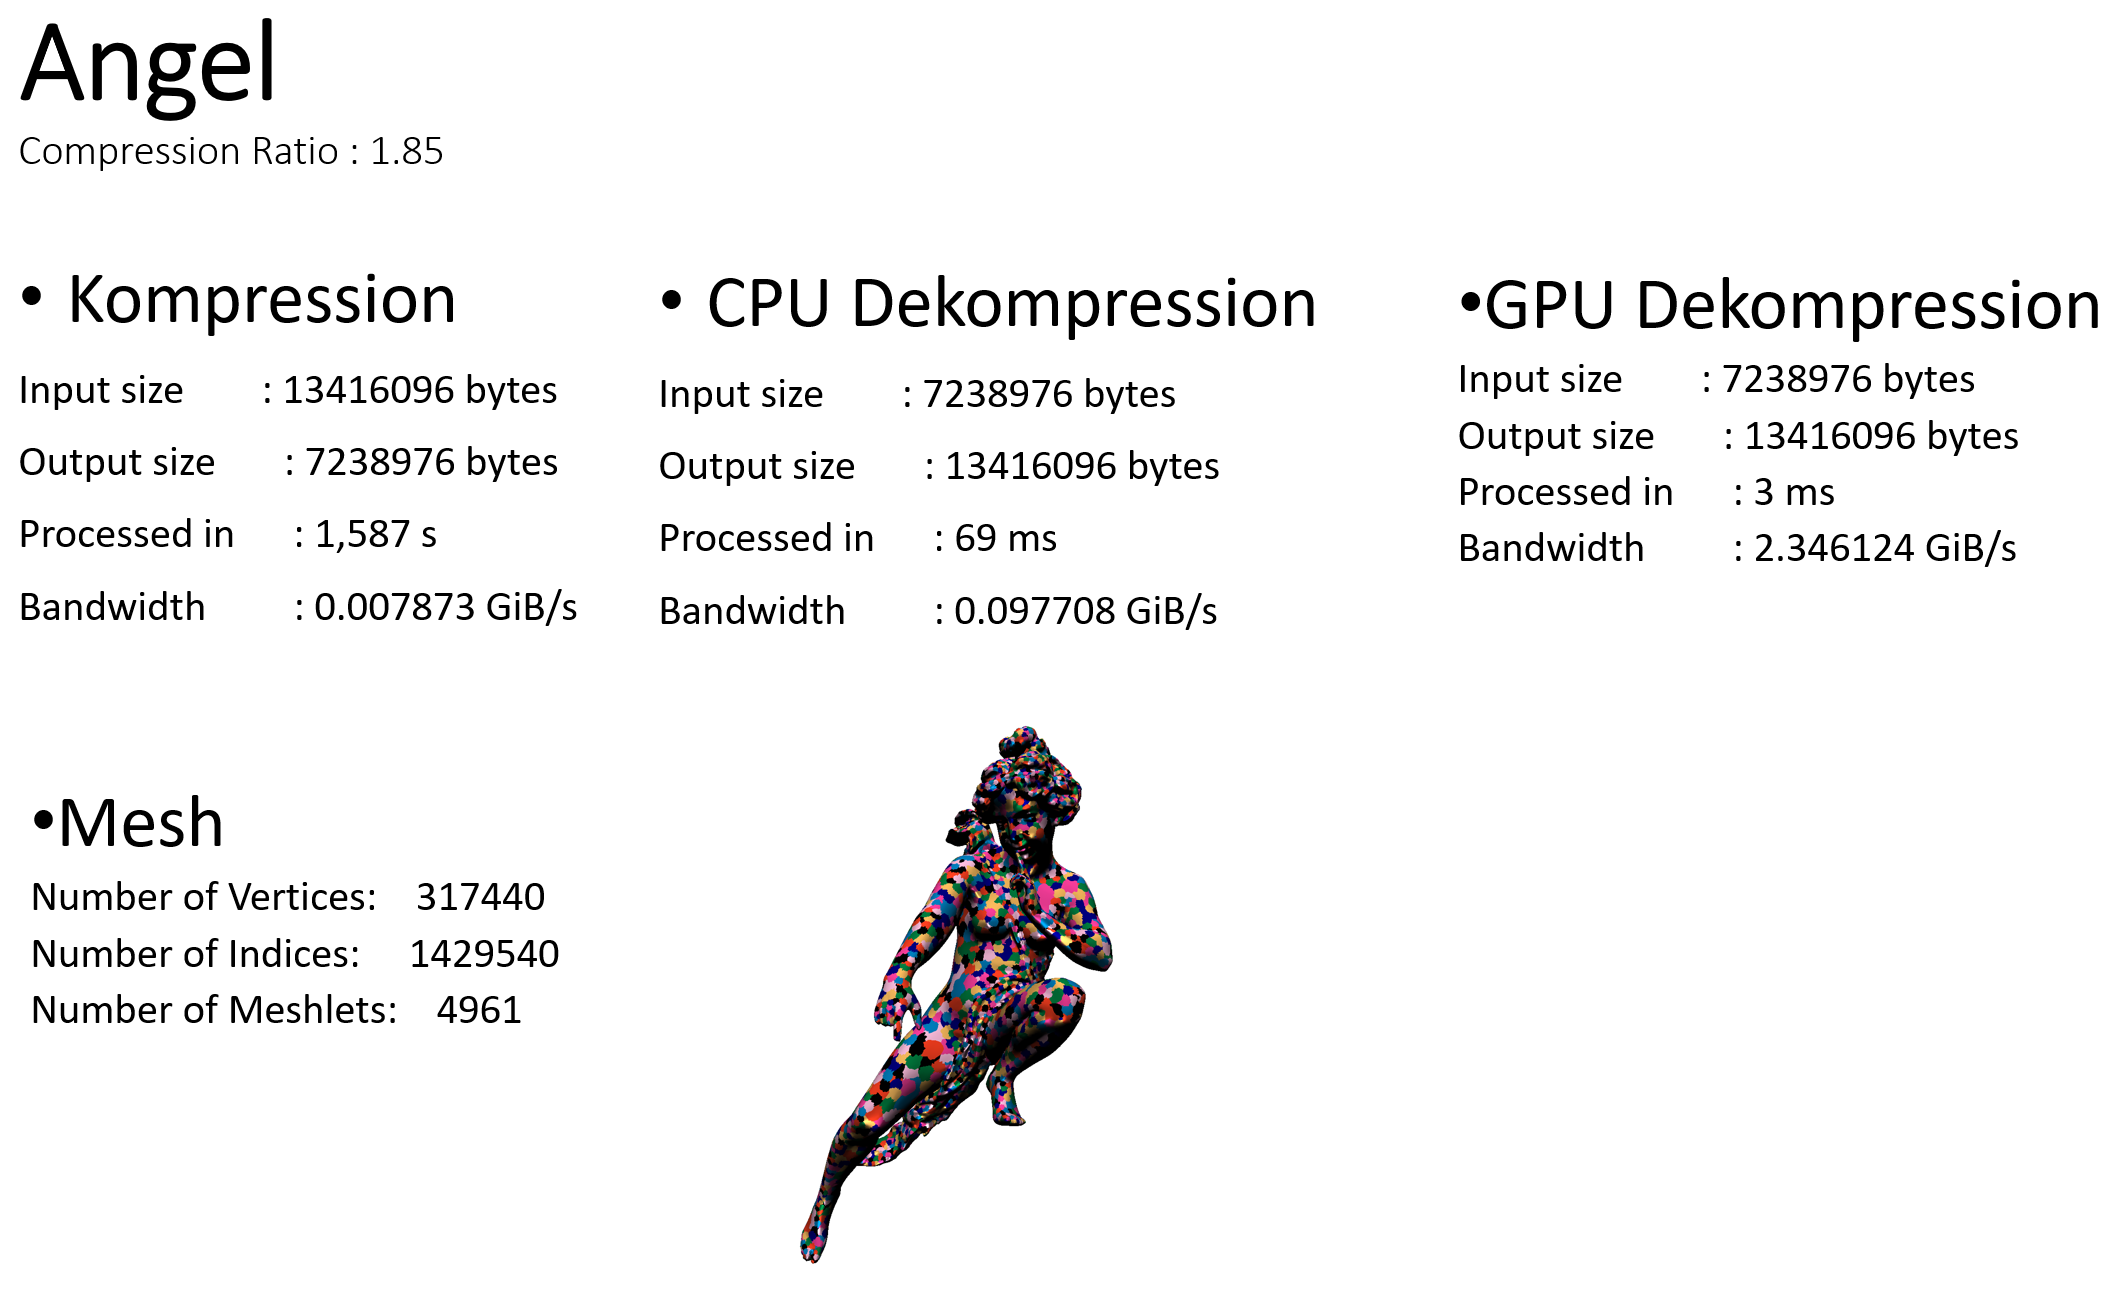
\includegraphics[scale=0.28]{Bilder/ergebnisse_full/angel.png}
\end{figure}
\begin{figure}[h]
  \centering  
  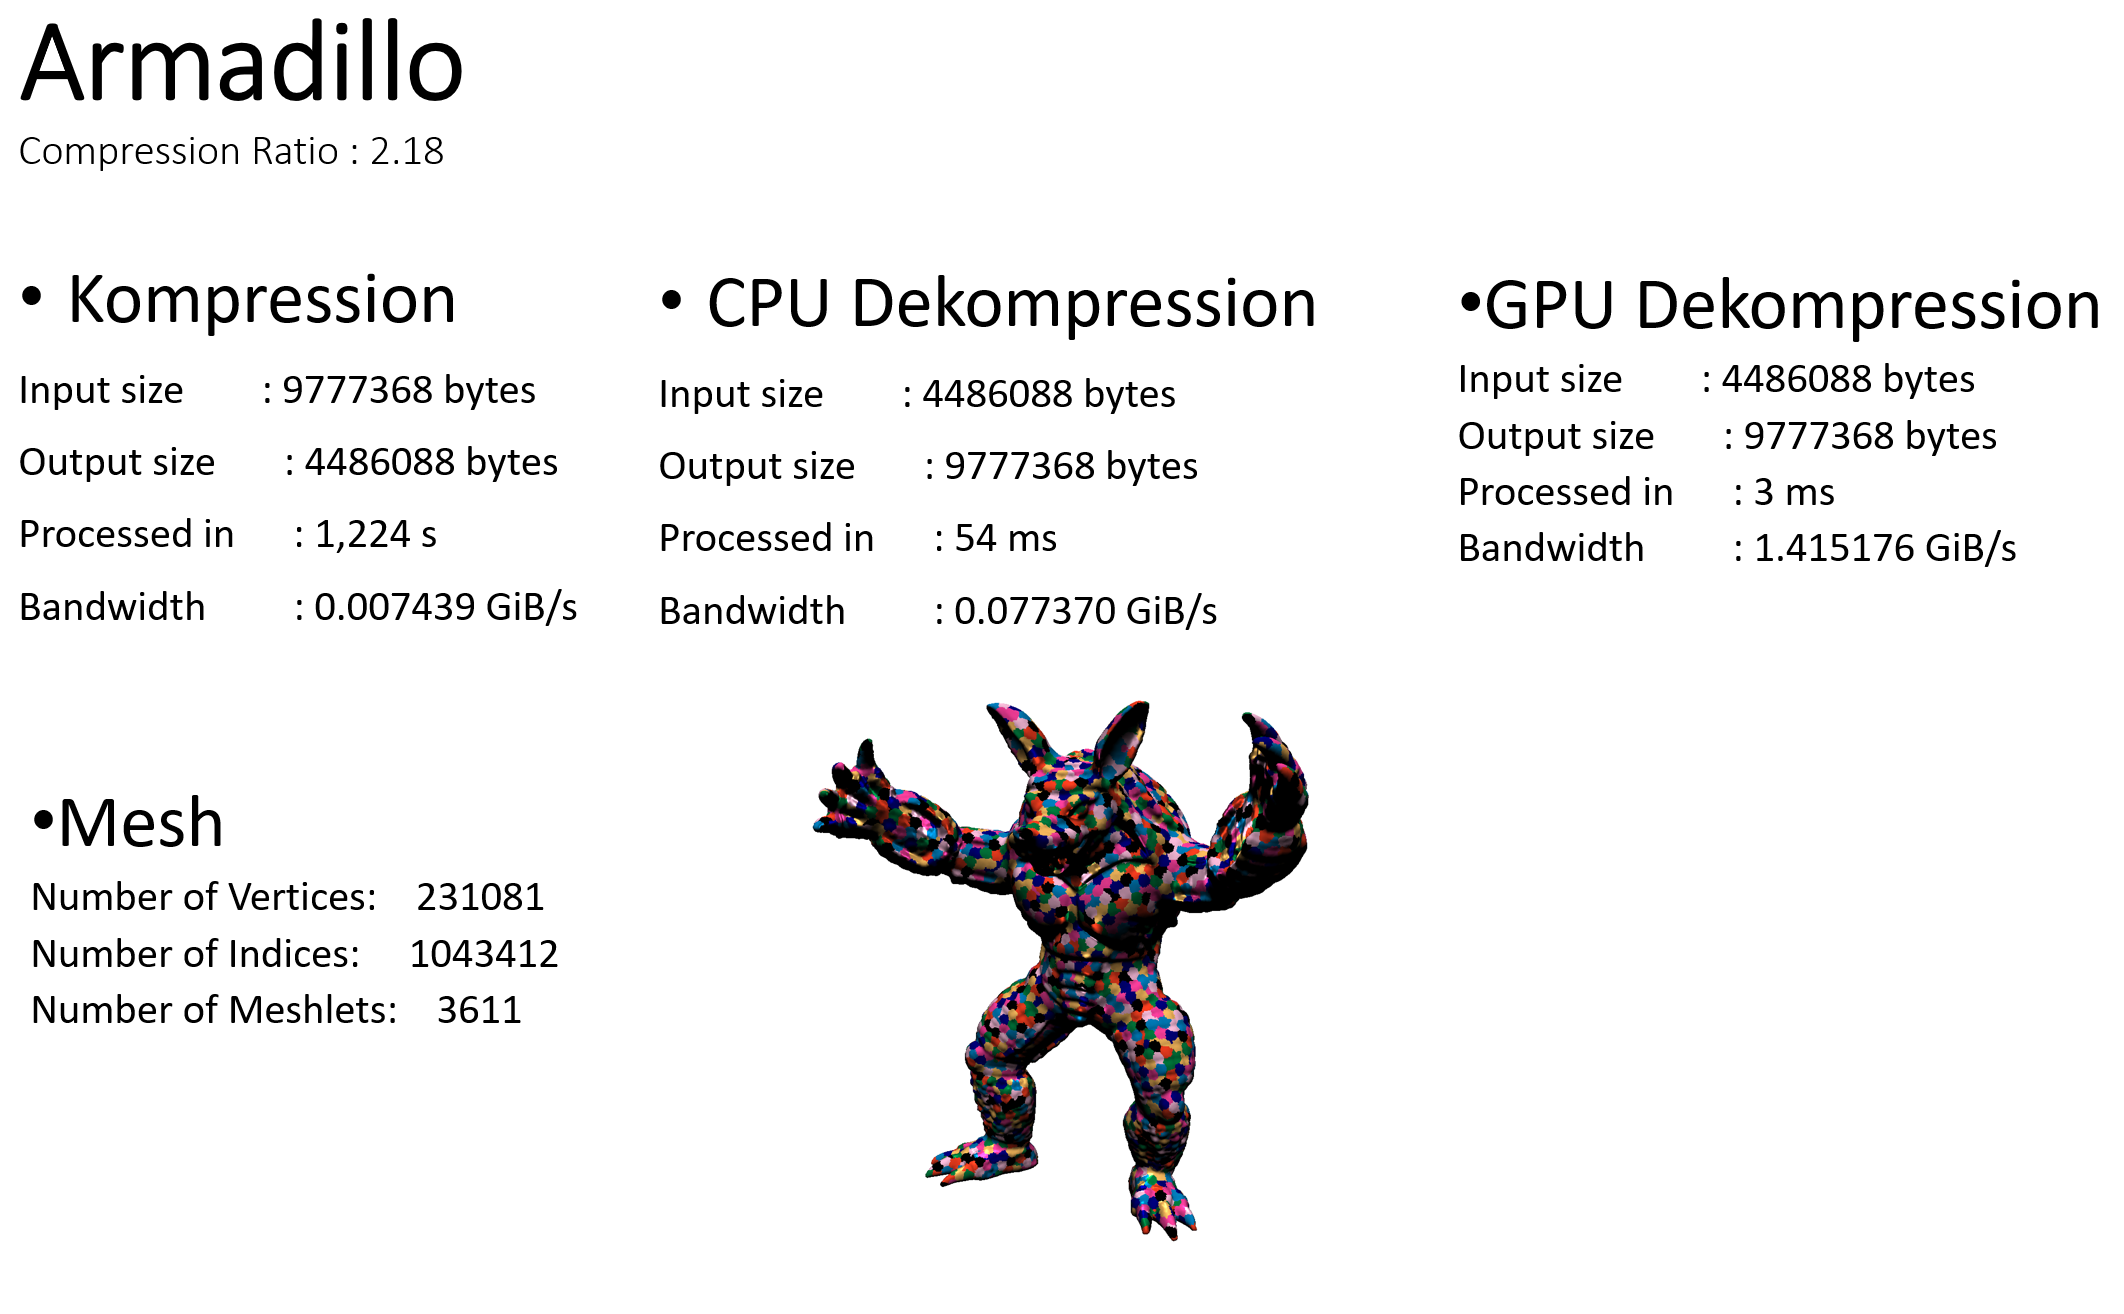
\includegraphics[scale=0.28]{Bilder/ergebnisse_full/armadillo.png}
\end{figure}
\begin{figure}[h]
  \centering  
  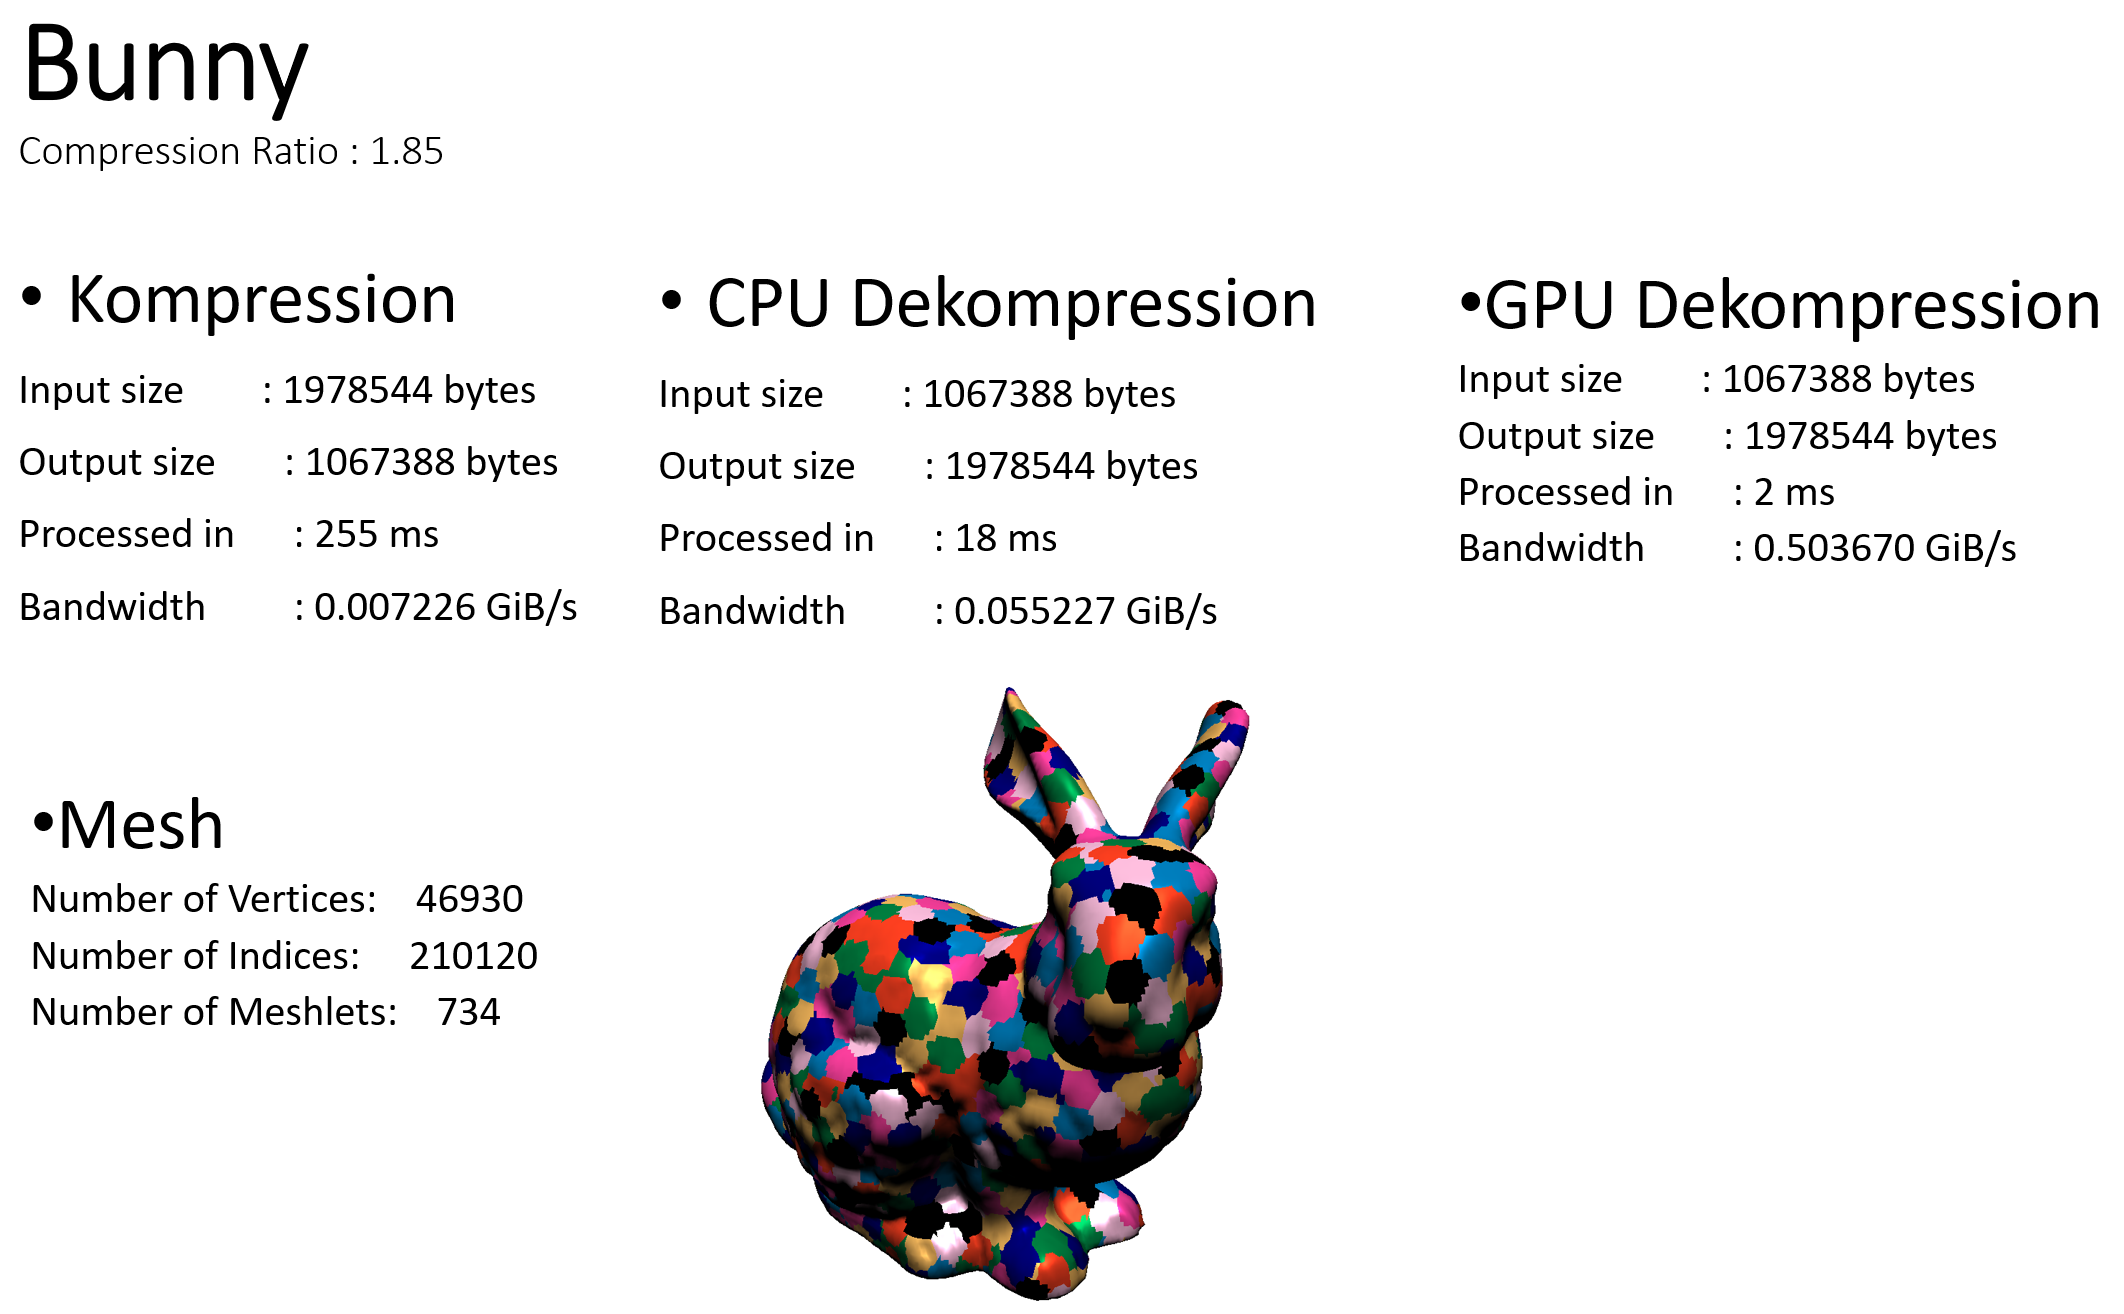
\includegraphics[scale=0.28]{Bilder/ergebnisse_full/bunny.png}
\end{figure}
\begin{figure}[h]
  \centering  
  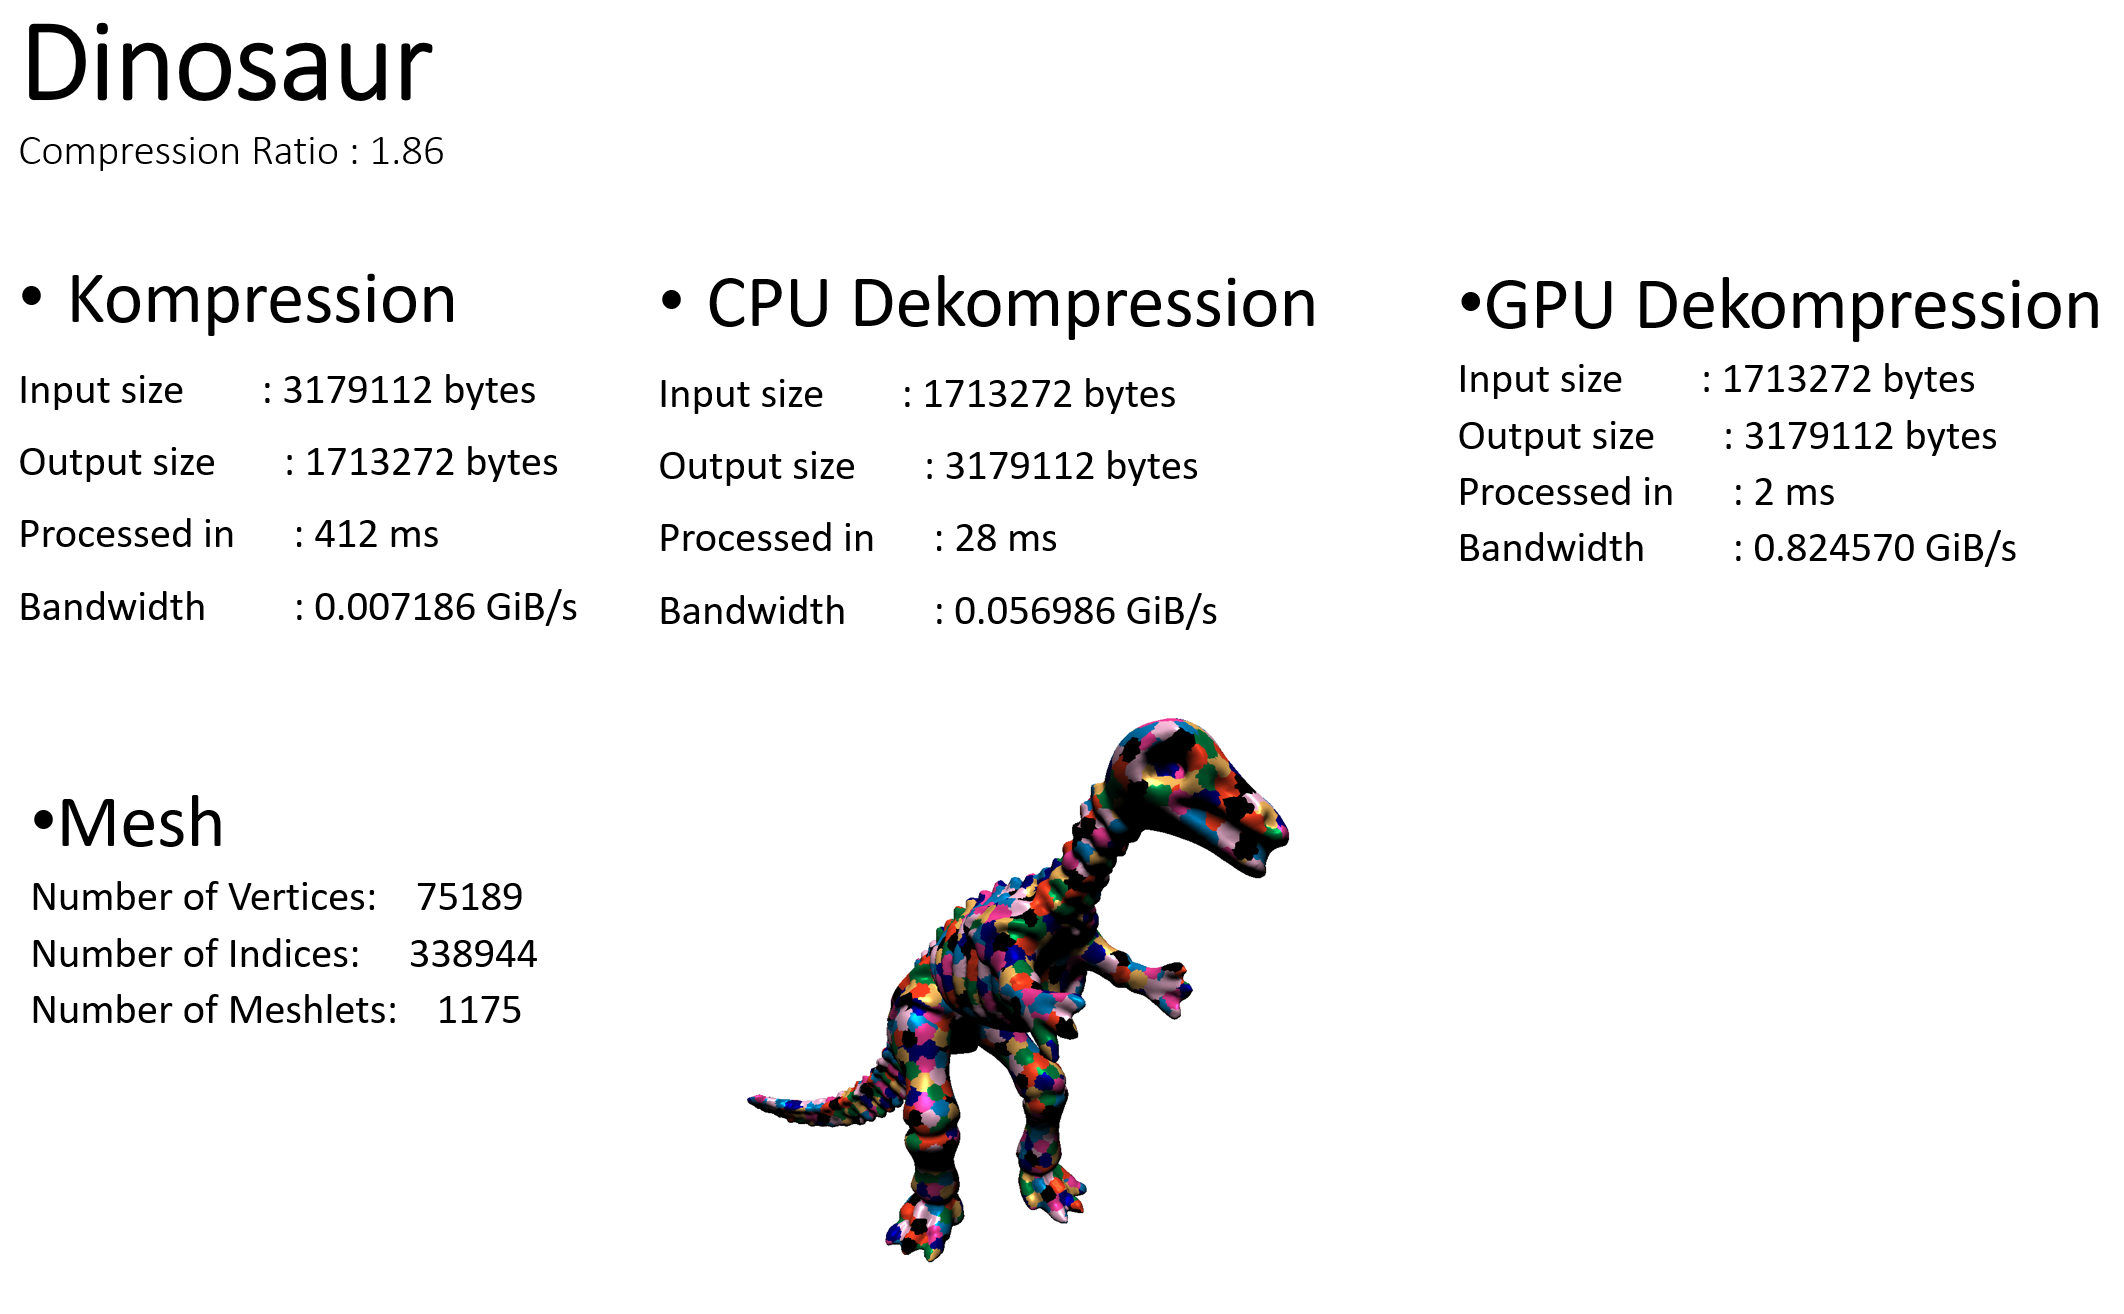
\includegraphics[scale=0.28]{Bilder/ergebnisse_full/dinosaur.png}
\end{figure}
\begin{figure}[h]
  \centering  
  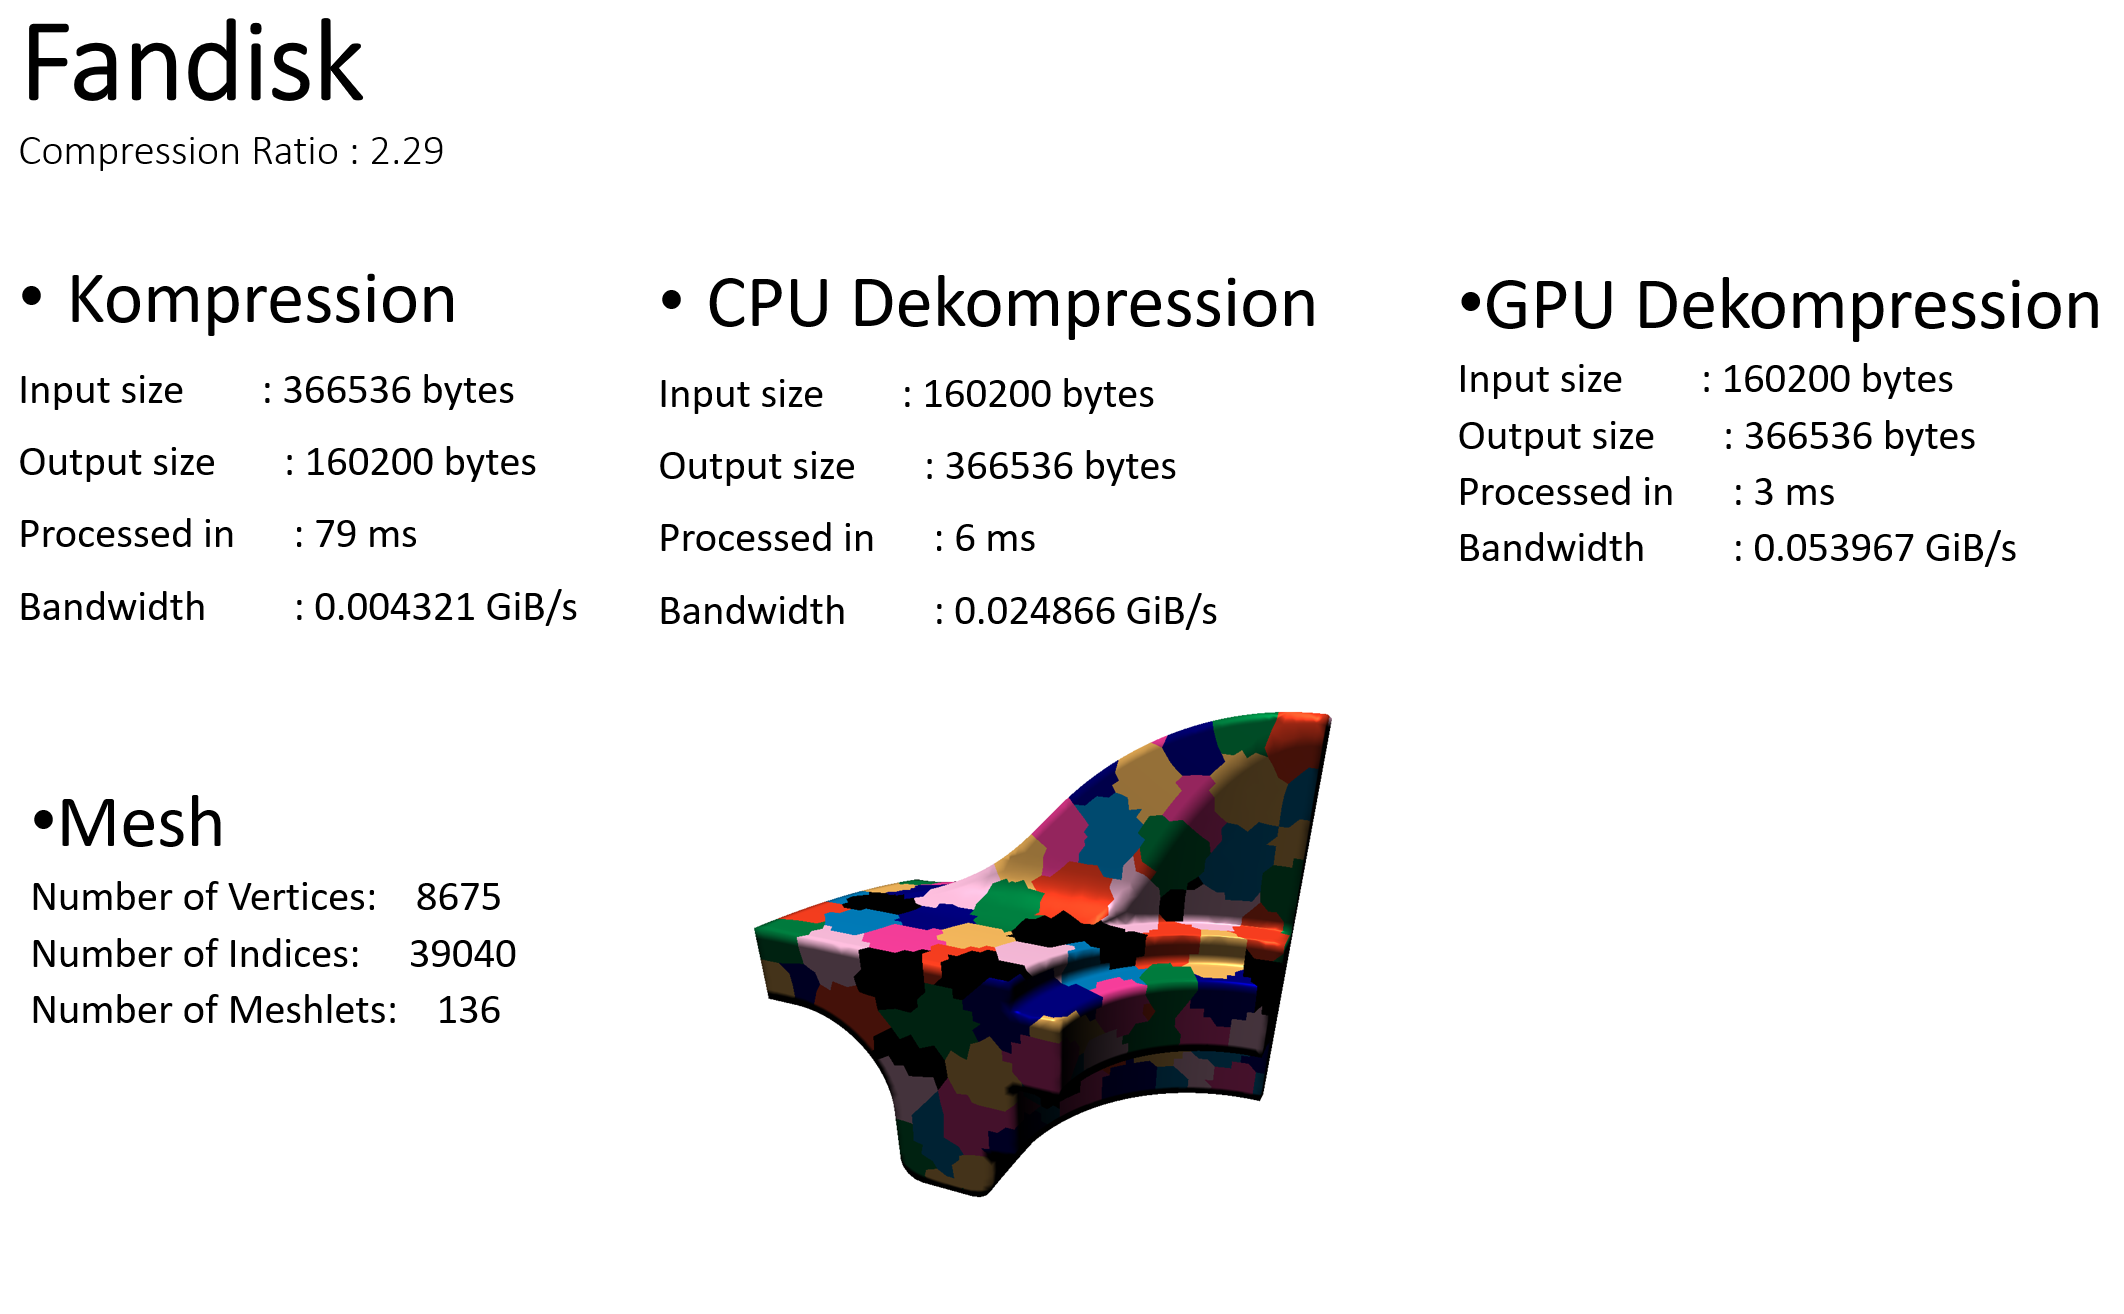
\includegraphics[scale=0.28]{Bilder/ergebnisse_full/fandisk.png}
\end{figure}
\begin{figure}[h]
  \centering  
  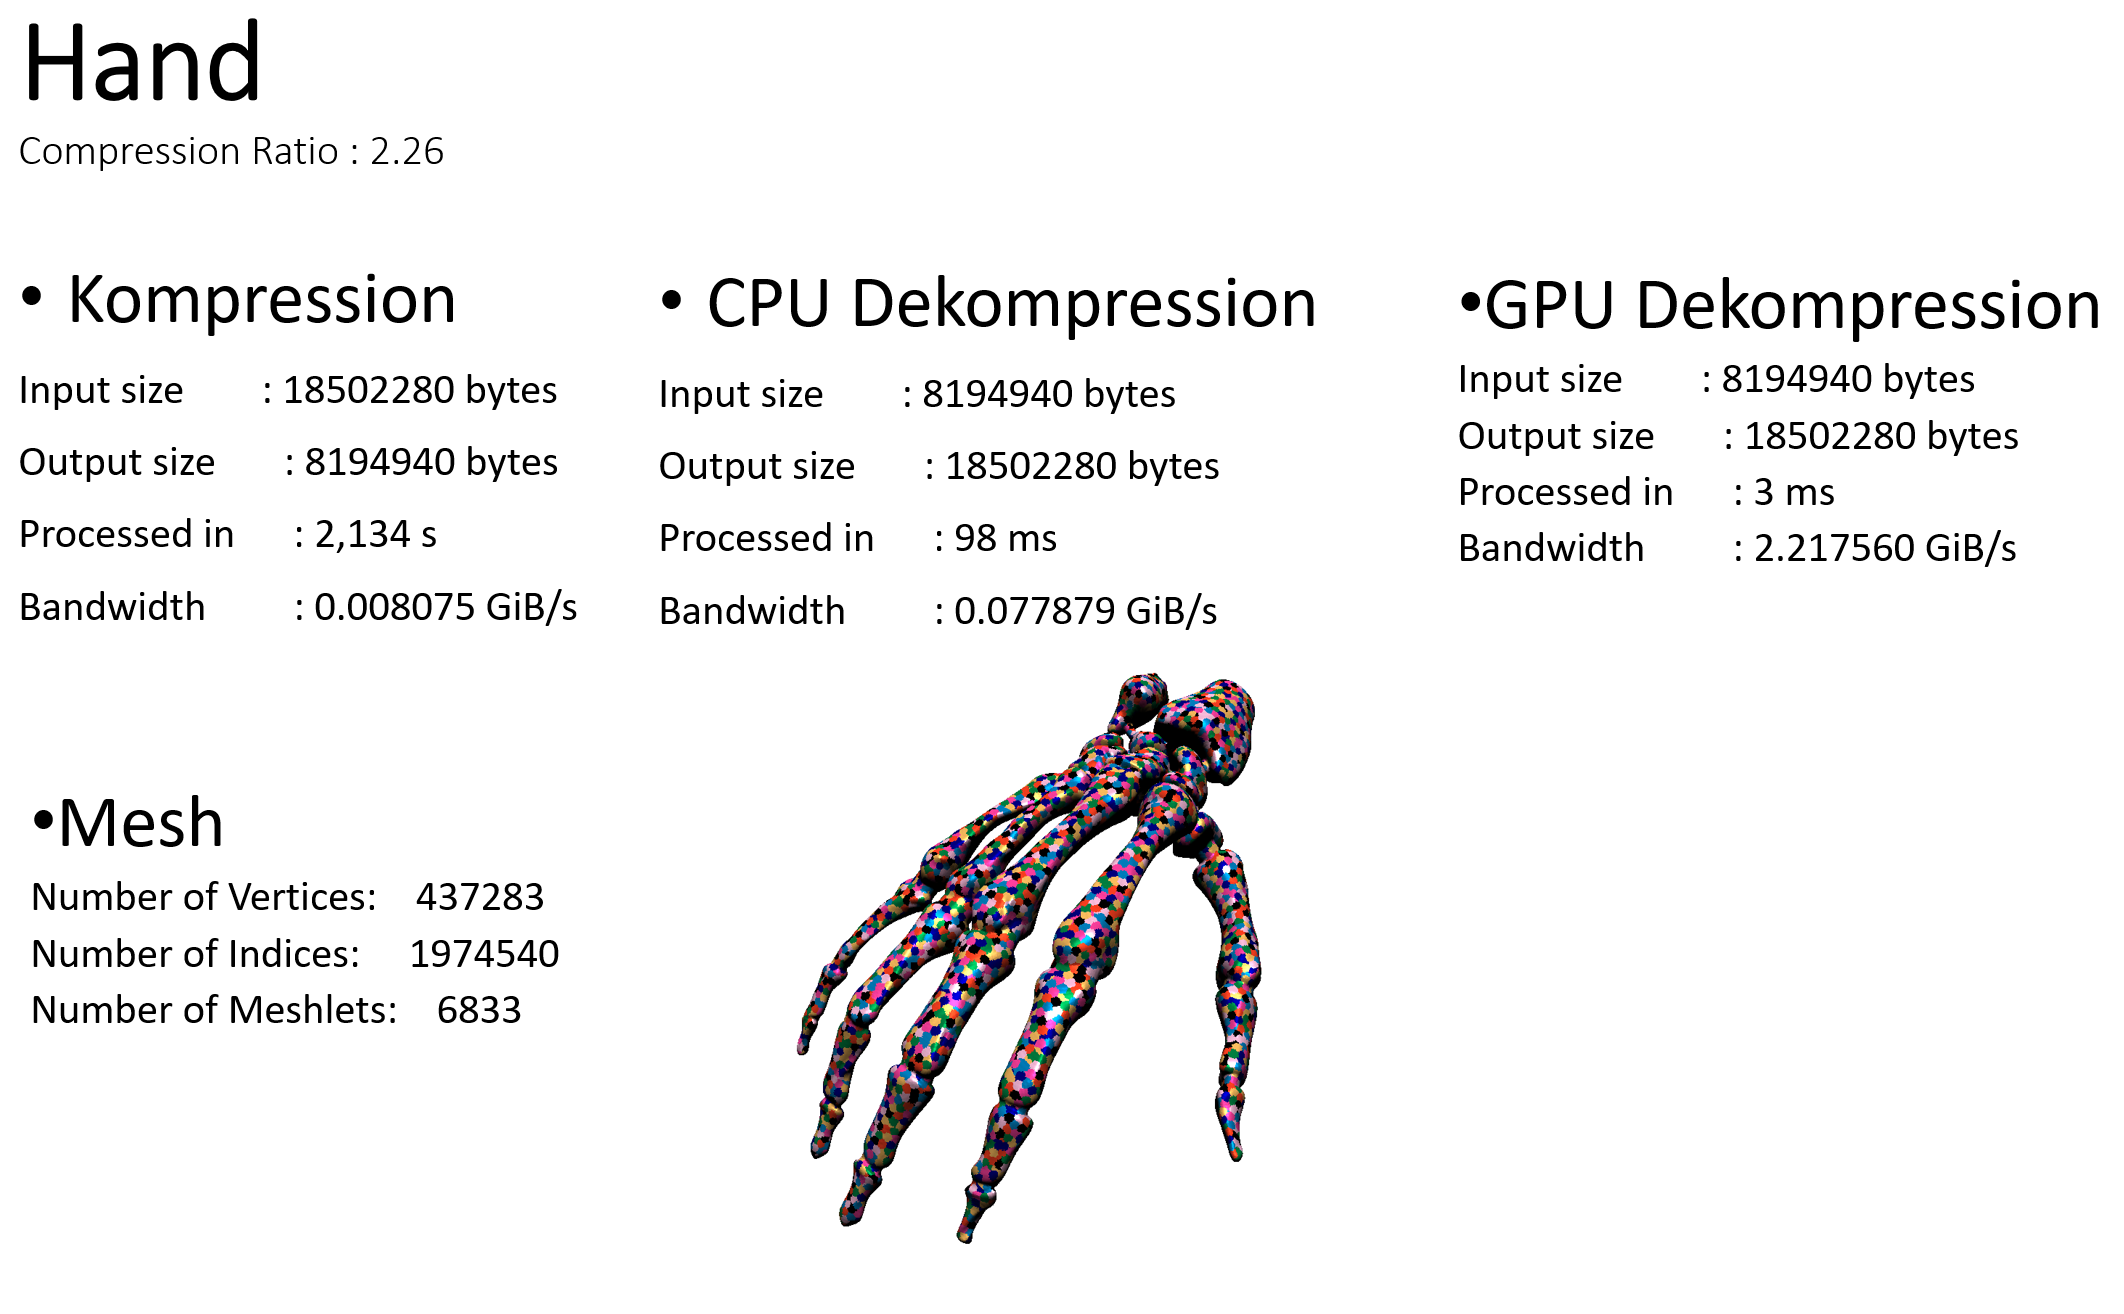
\includegraphics[scale=0.28]{Bilder/ergebnisse_full/hand.png}
\end{figure}
\begin{figure}[h]
  \centering  
  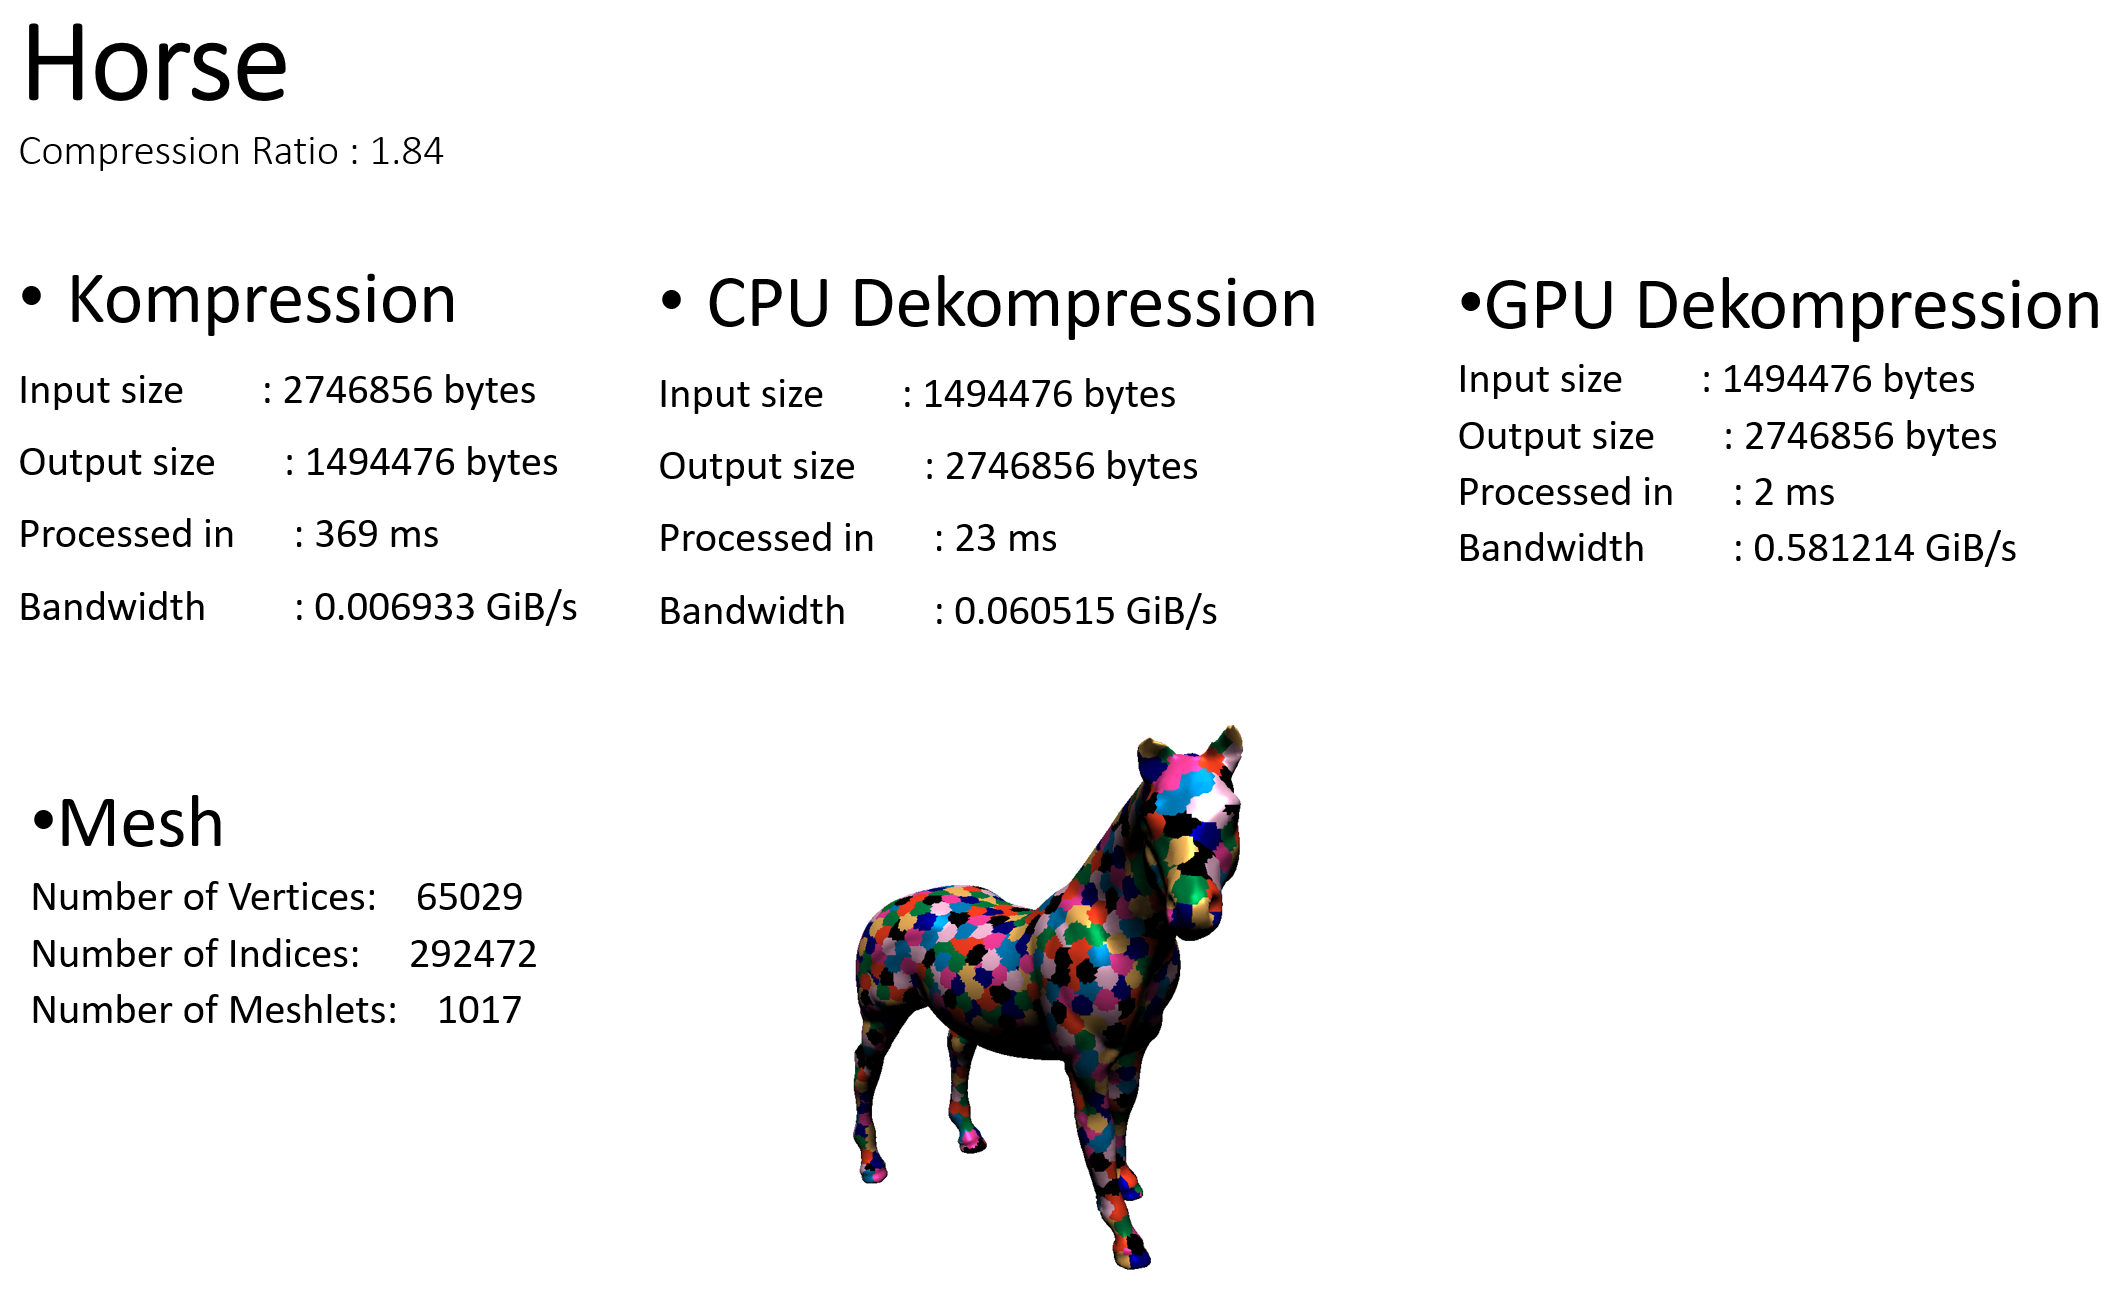
\includegraphics[scale=0.28]{Bilder/ergebnisse_full/horse.png}
\end{figure}
\begin{figure}[h]
  \centering  
  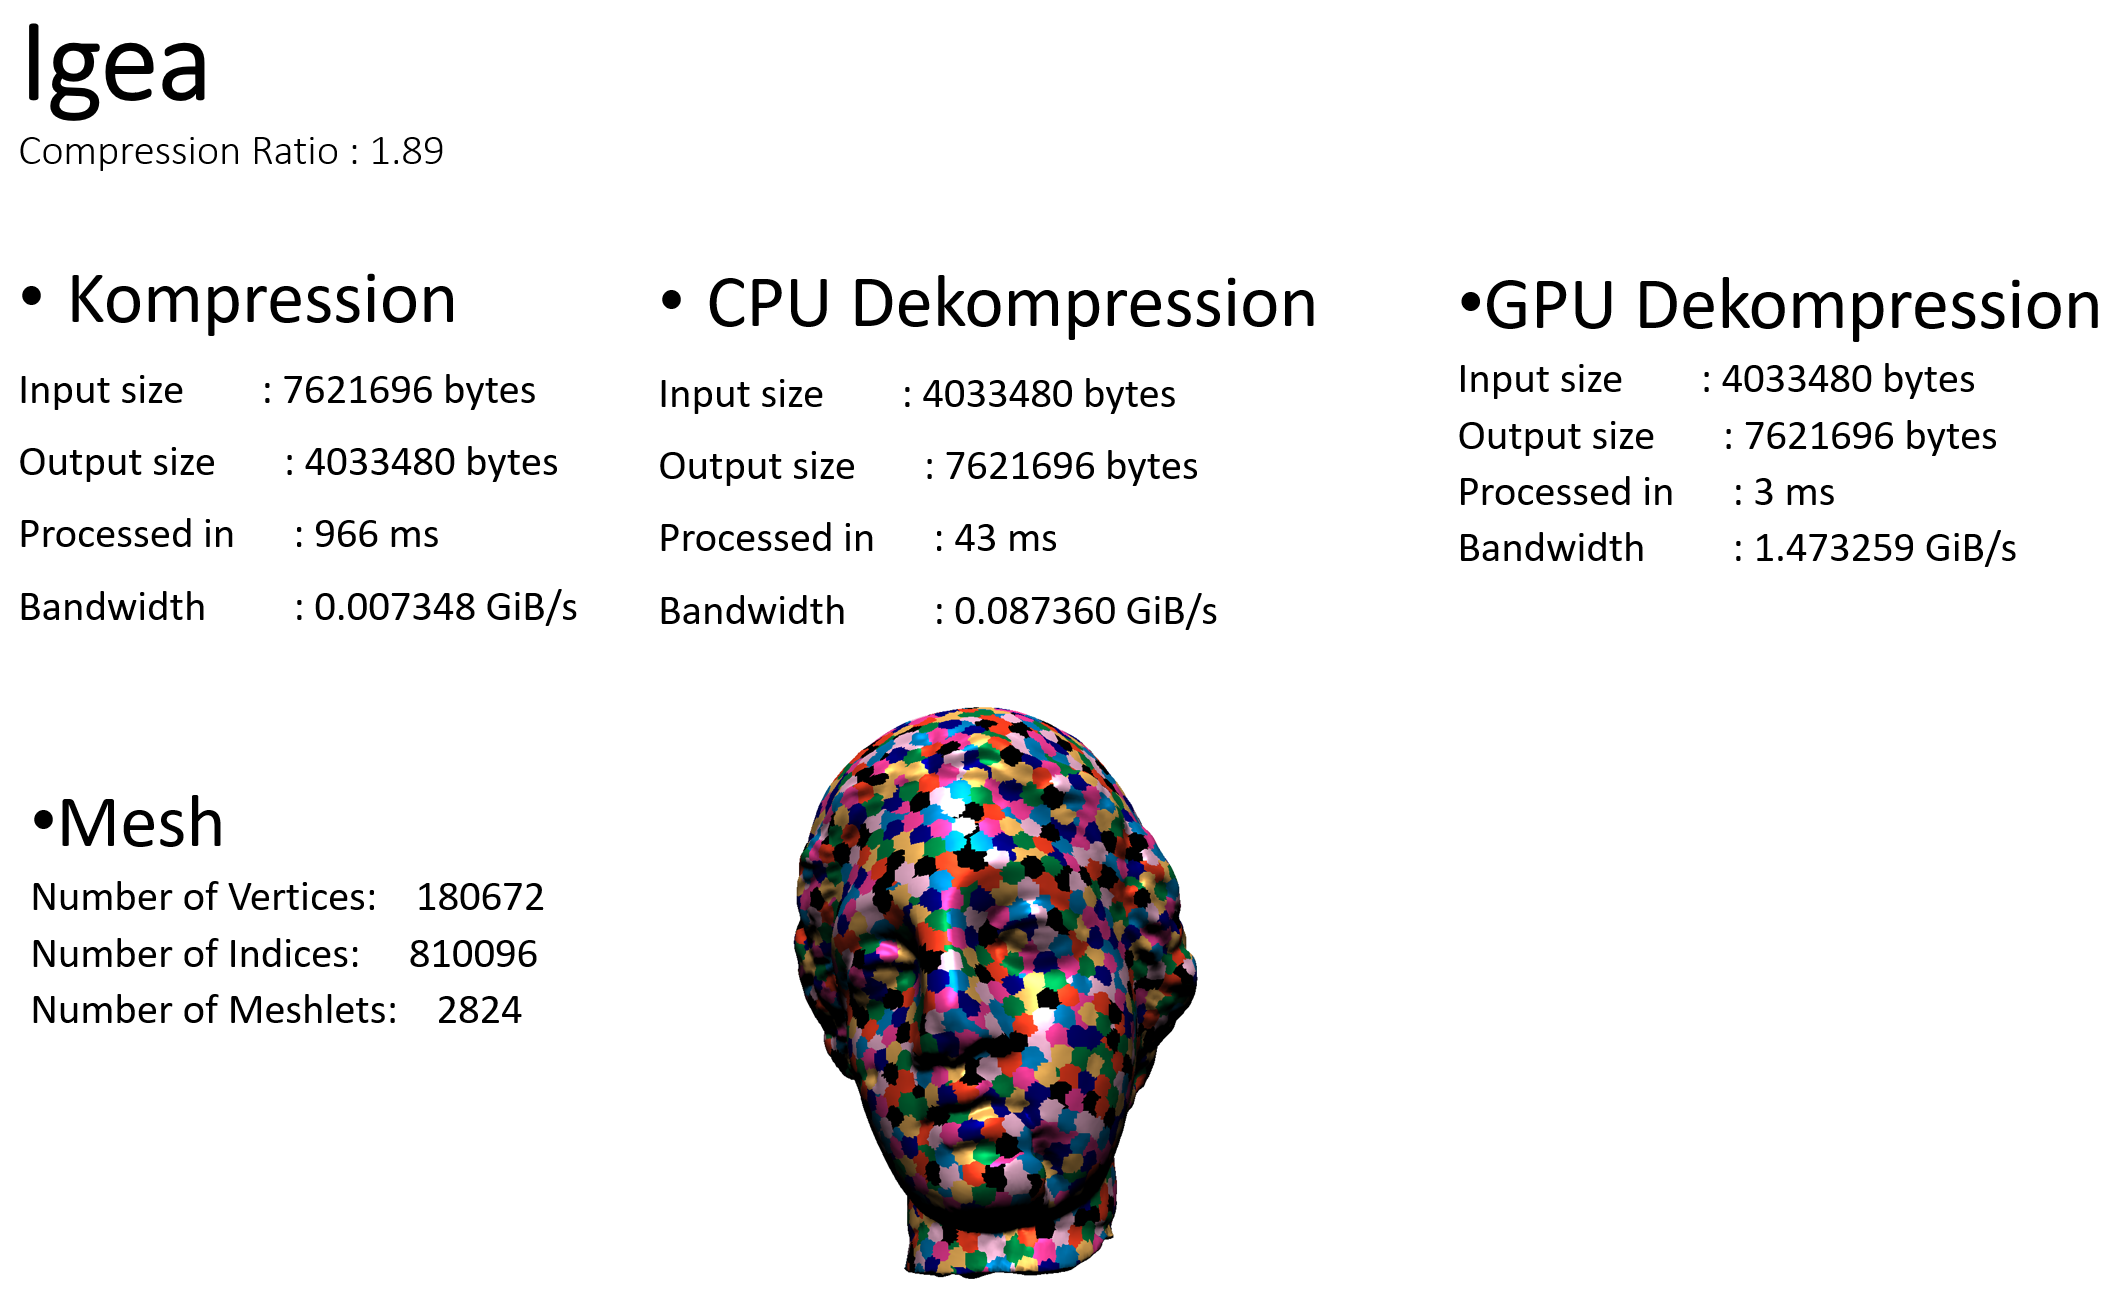
\includegraphics[scale=0.28]{Bilder/ergebnisse_full/igea.png}
\end{figure}
\begin{figure}[h]
  \centering  
  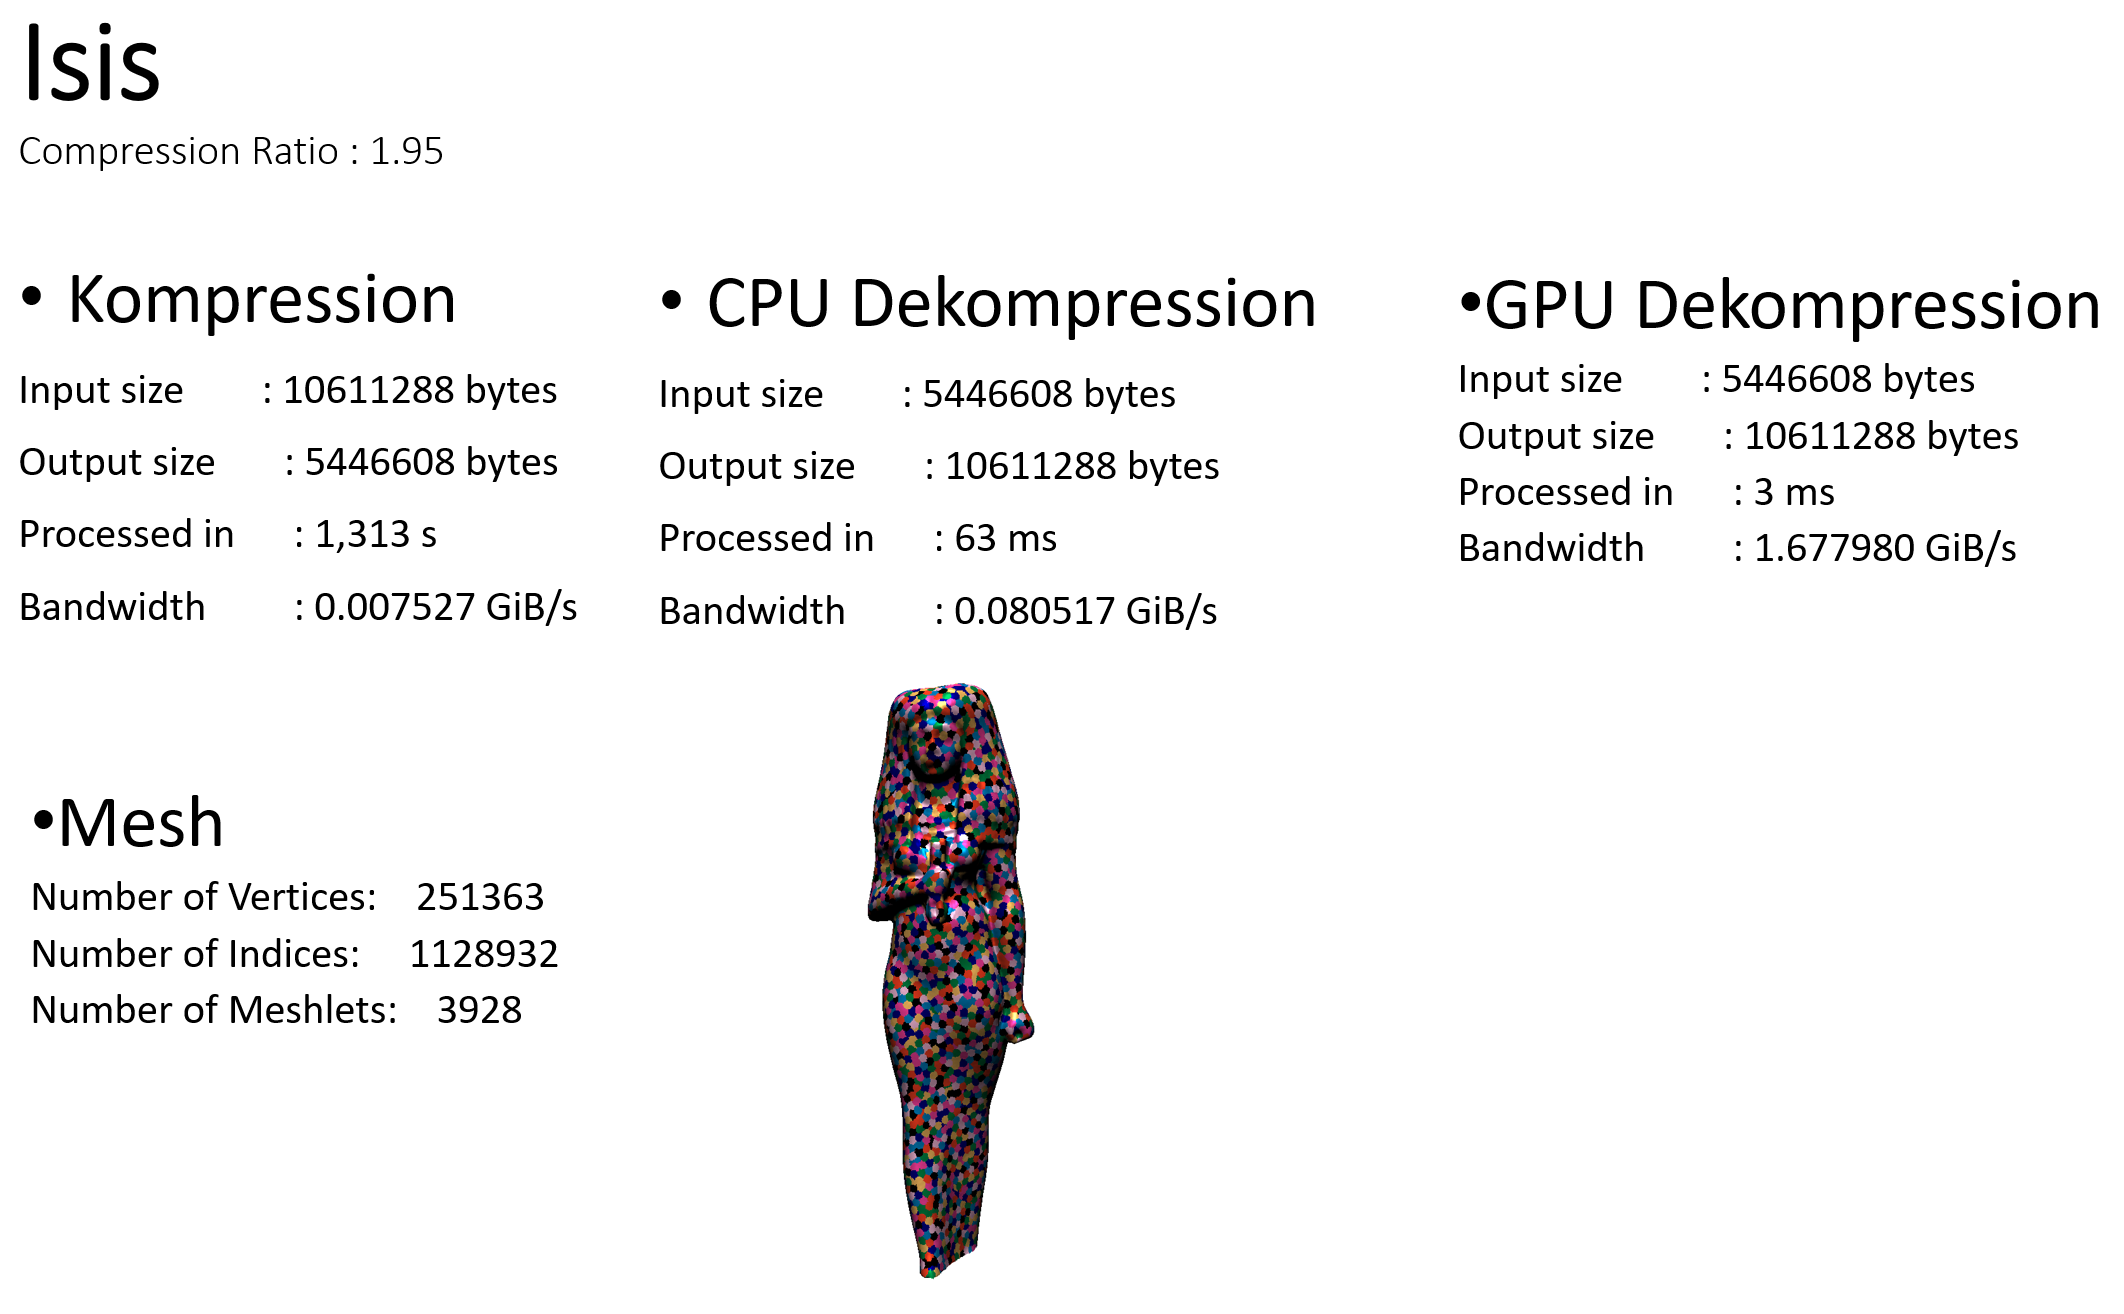
\includegraphics[scale=0.28]{Bilder/ergebnisse_full/isis.png}
\end{figure}
\begin{figure}[h]
  \centering  
  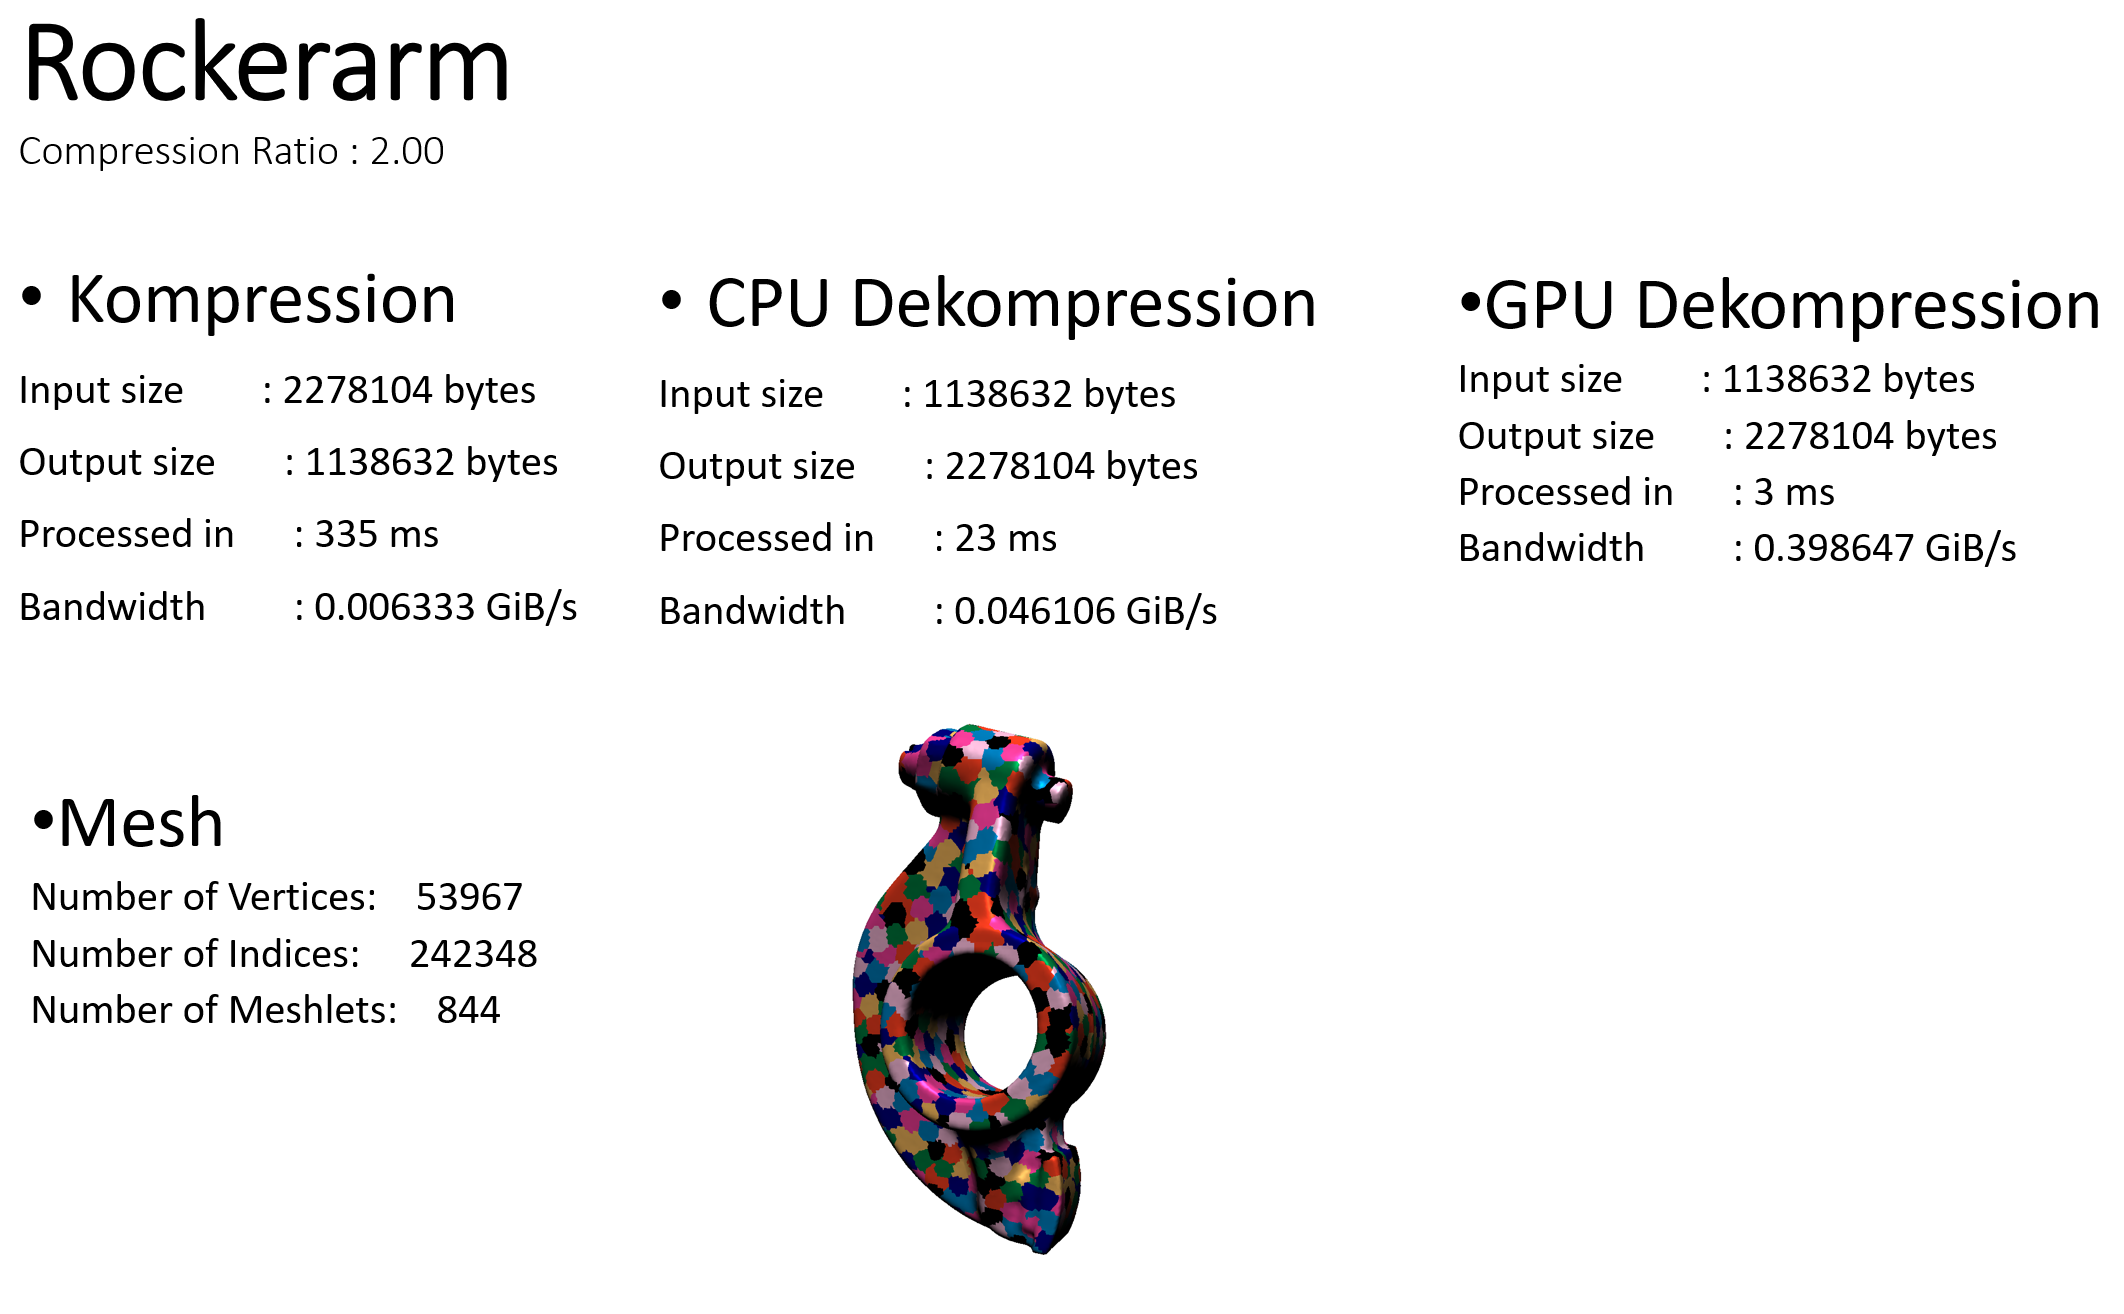
\includegraphics[scale=0.28]{Bilder/ergebnisse_full/rockerarm.png}
\end{figure}
\begin{figure}[h]
  \centering  
  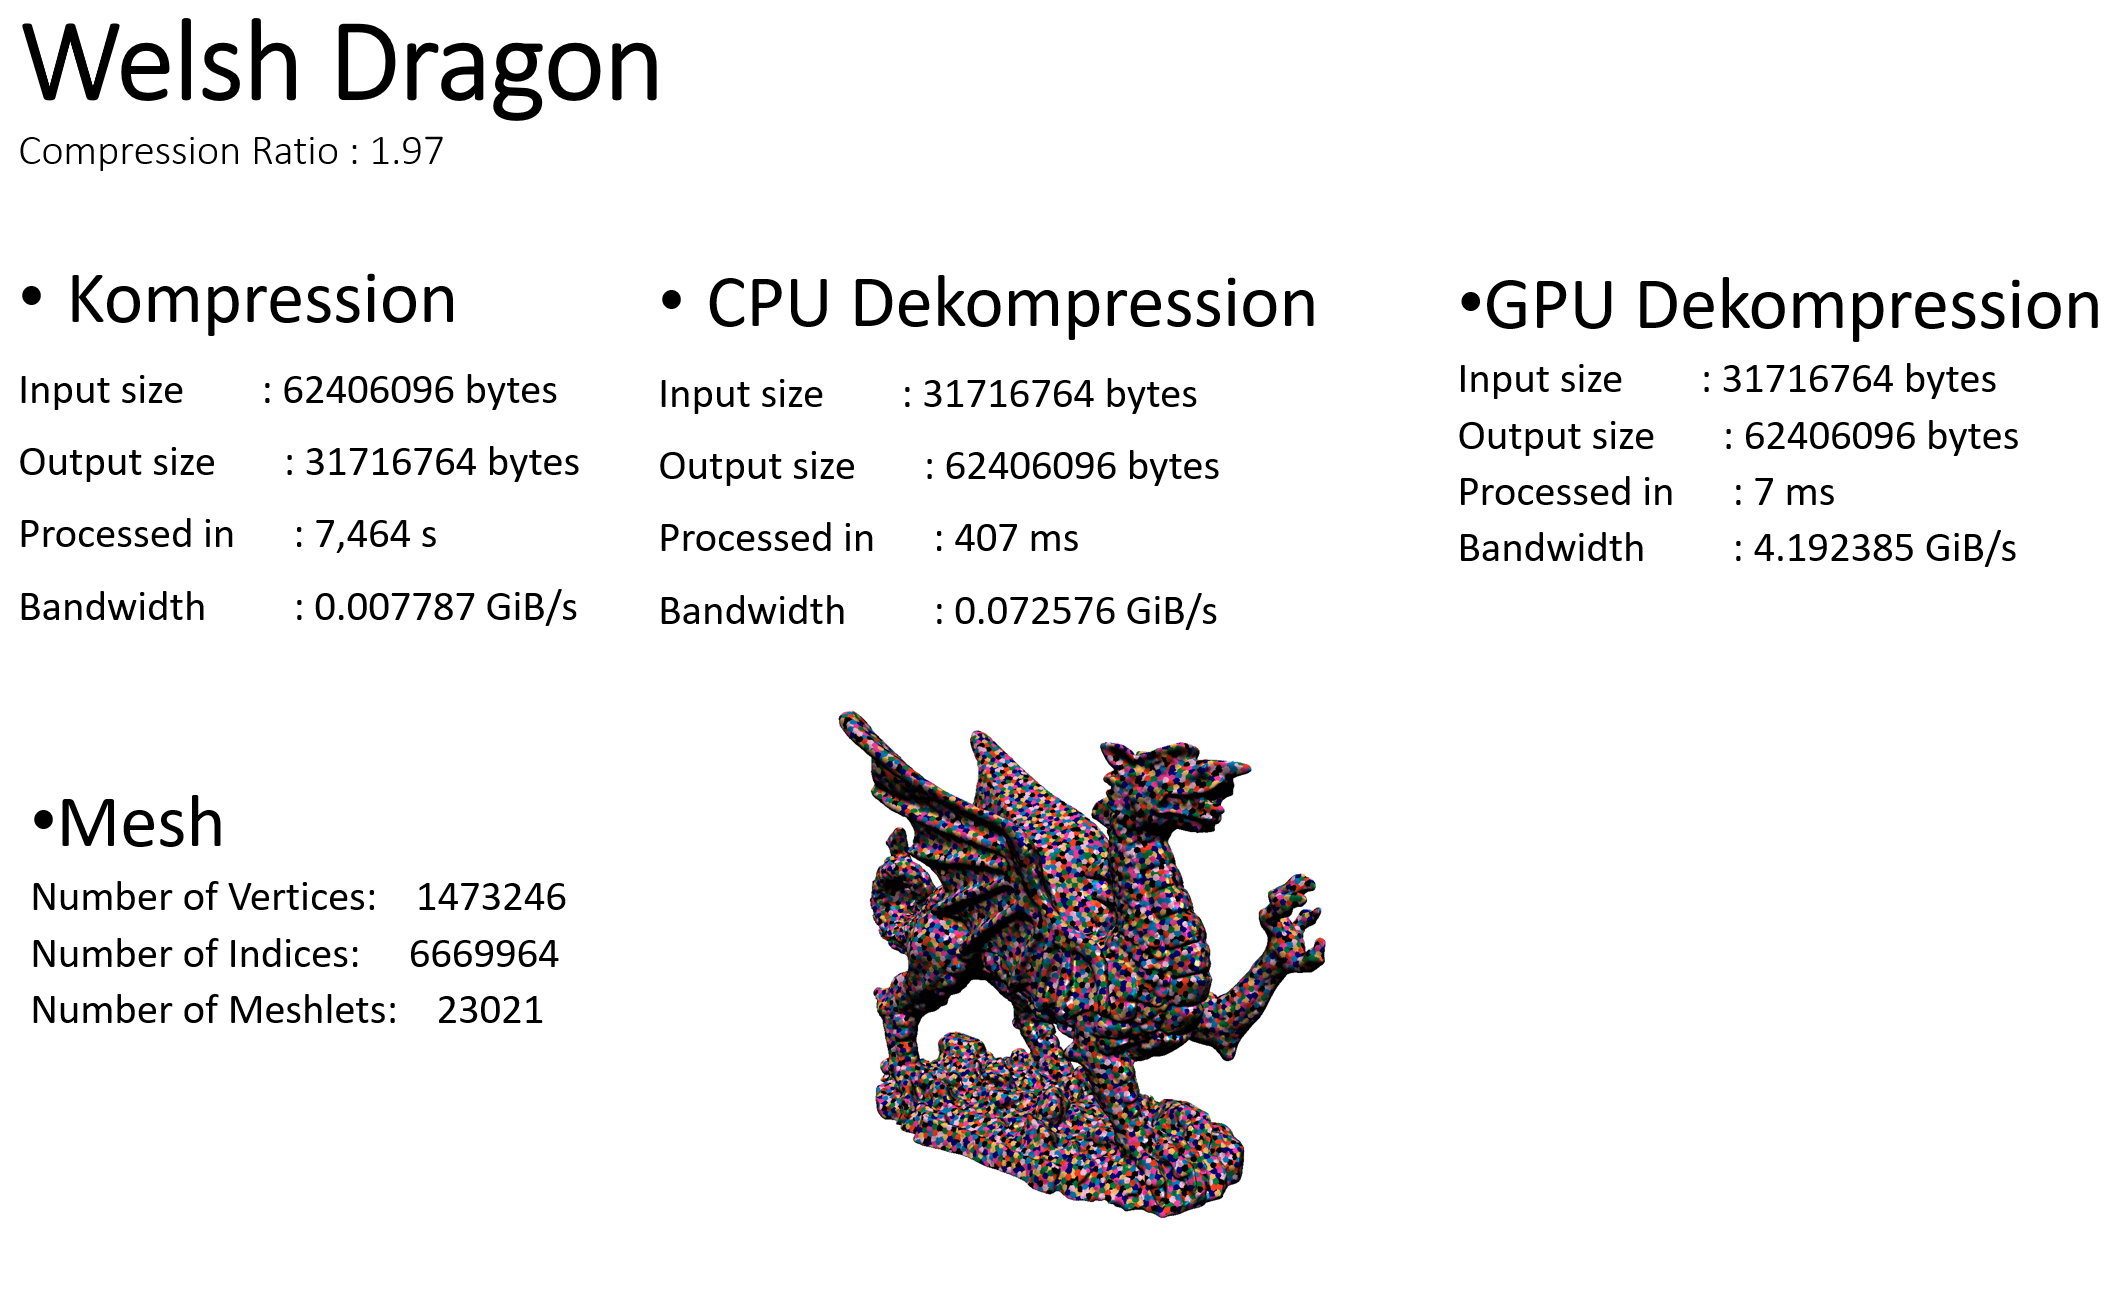
\includegraphics[scale=0.28]{Bilder/ergebnisse_full/welshdragon.png}
\end{figure}
\begin{figure}[h]
  \centering  
  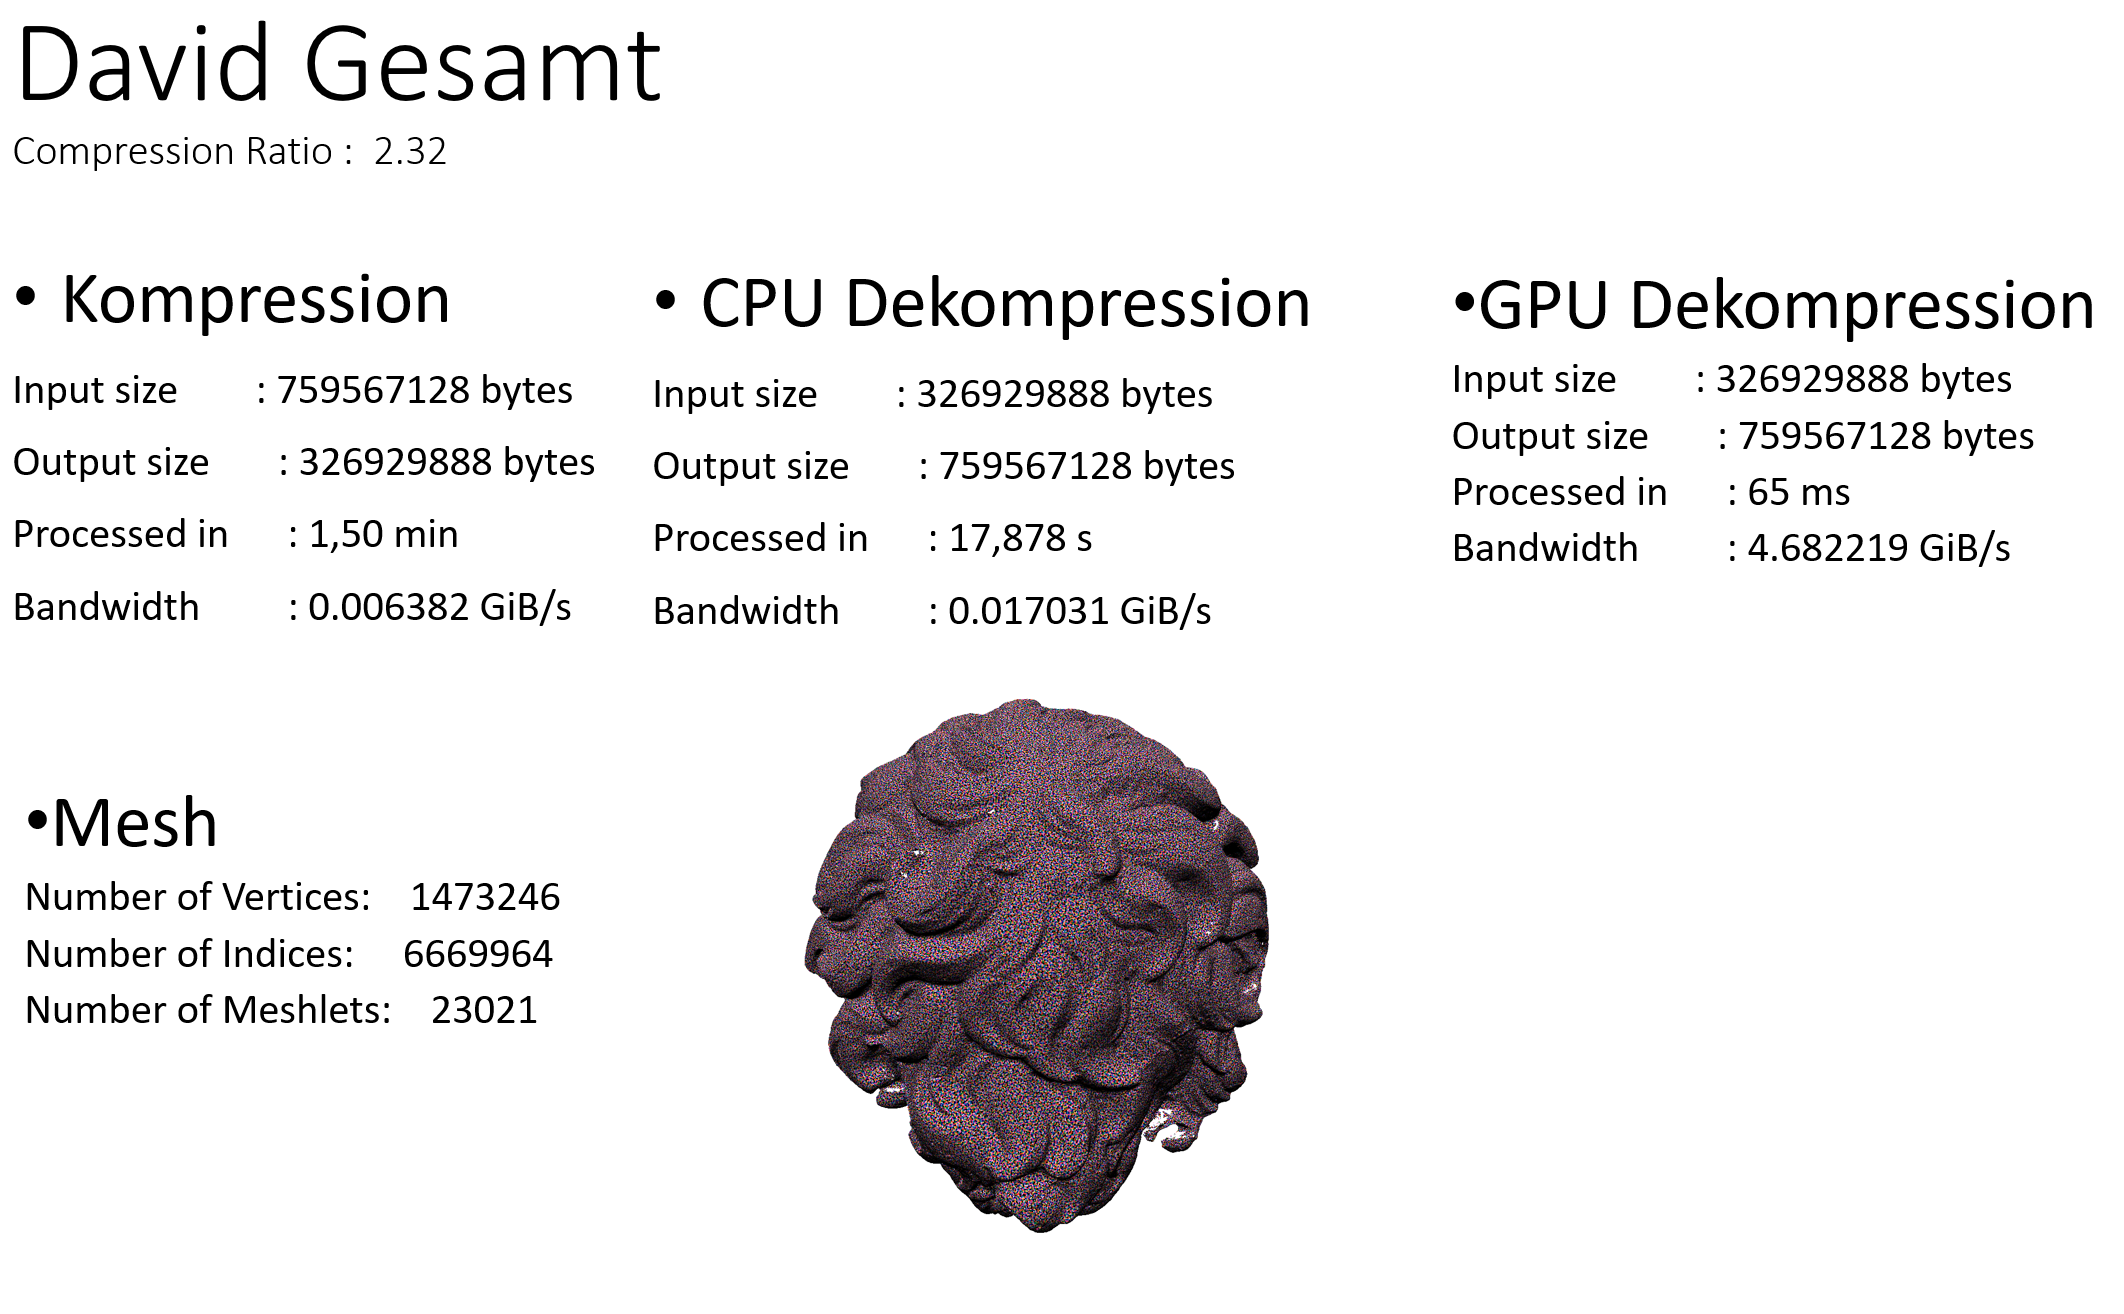
\includegraphics[scale=0.28]{Bilder/ergebnisse_full/david.png}
\end{figure}
\clearpage
\subsection{Ergebnisse mit Quantisierung}
\begin{figure}[h]
  \centering  
  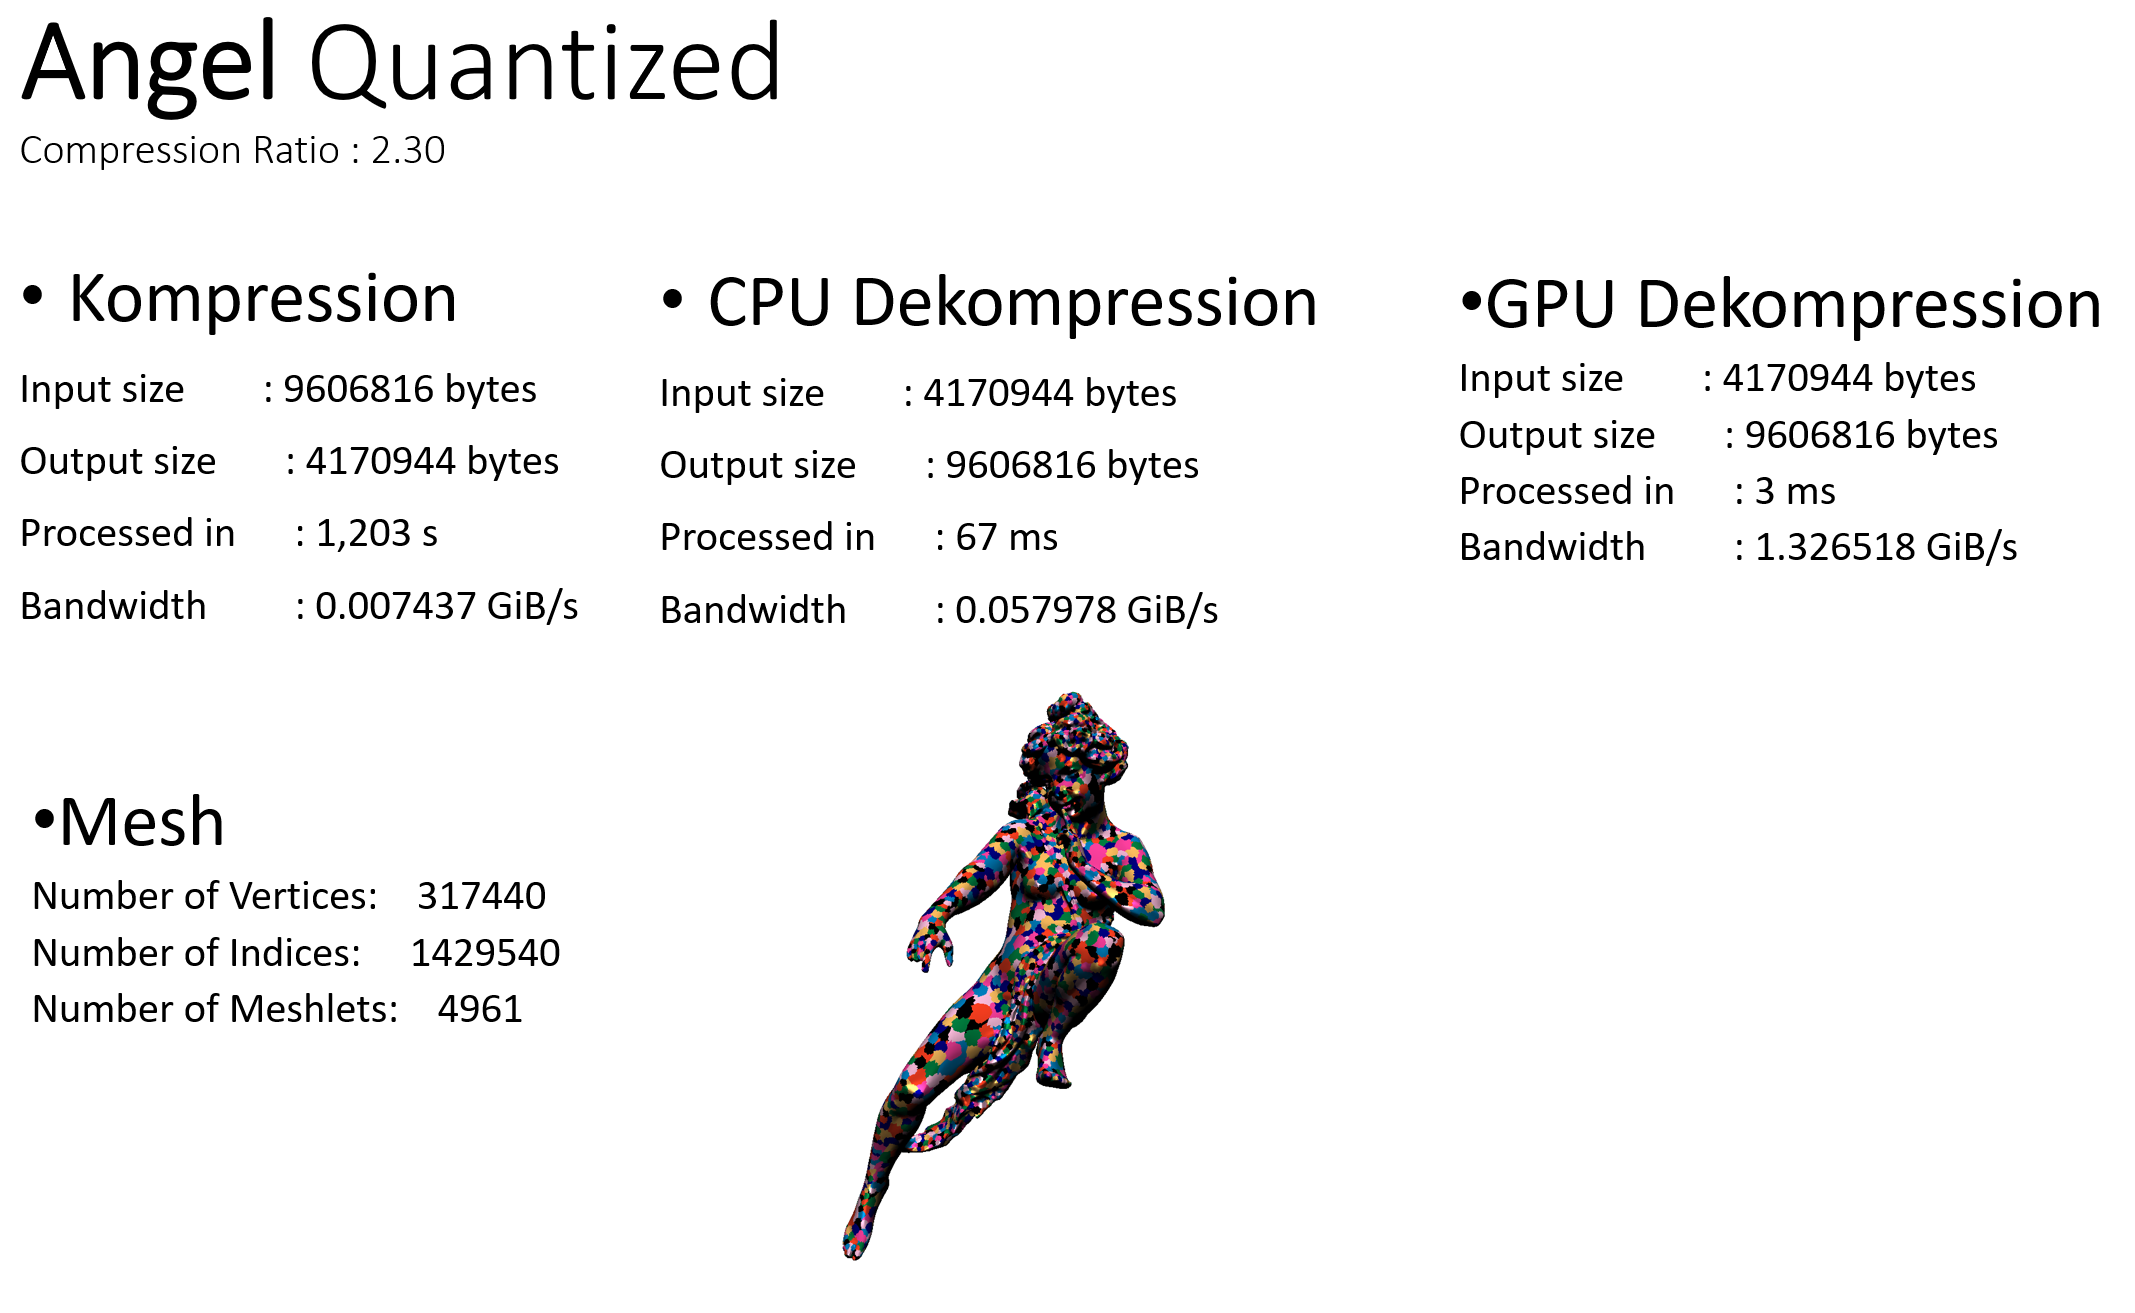
\includegraphics[scale=0.28]{Bilder/ergebnisse_full/angel_quantized.png}
\end{figure}
\begin{figure}[h]
  \centering  
  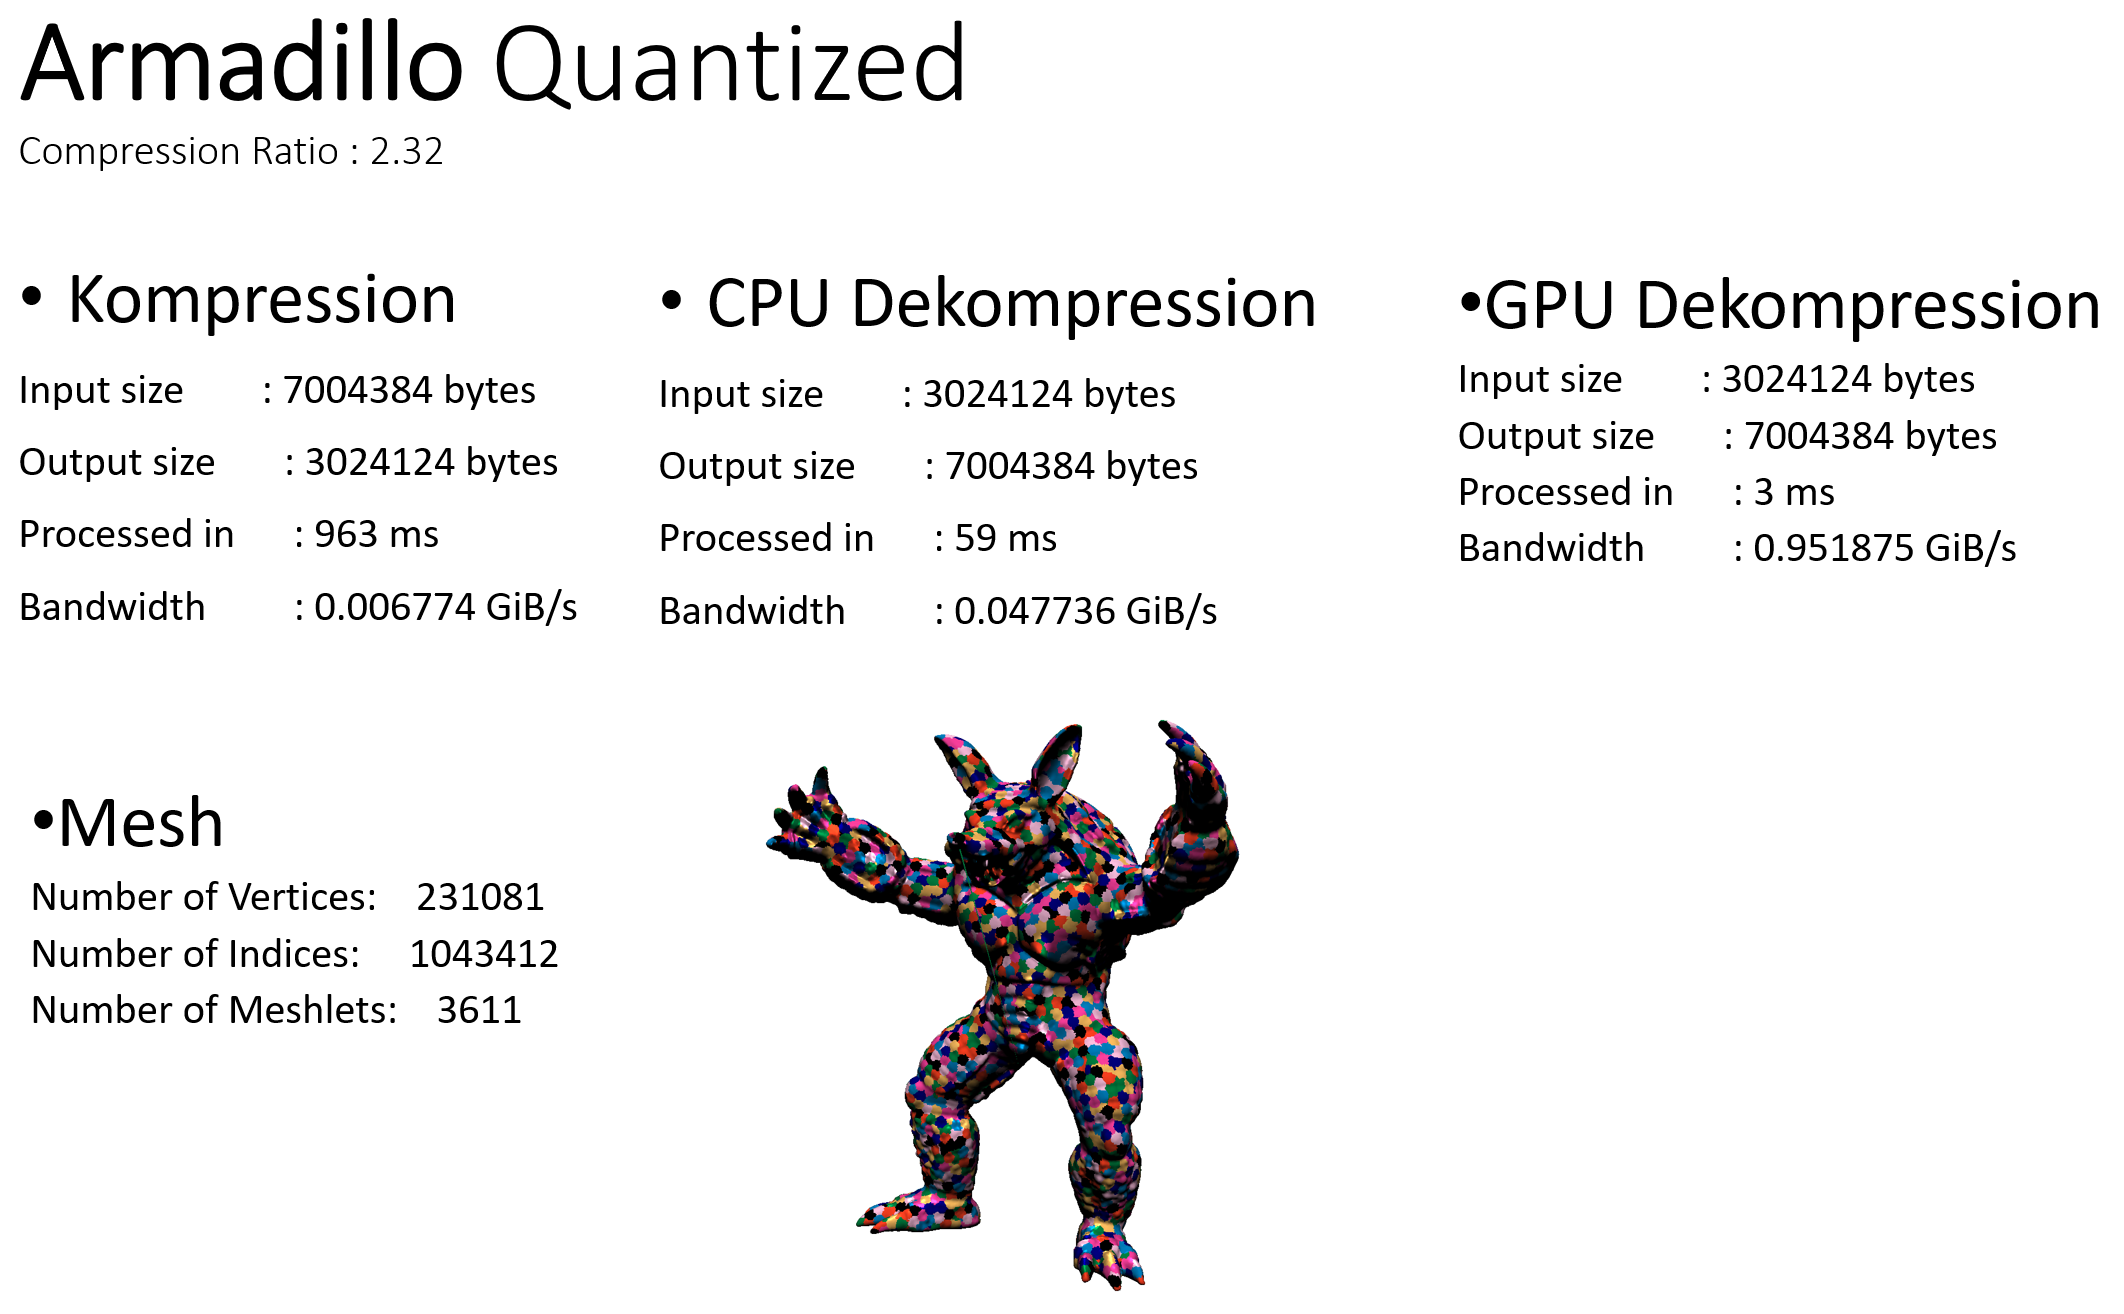
\includegraphics[scale=0.28]{Bilder/ergebnisse_full/armadillo_quantized.png}
\end{figure}
\begin{figure}[h]
  \centering  
  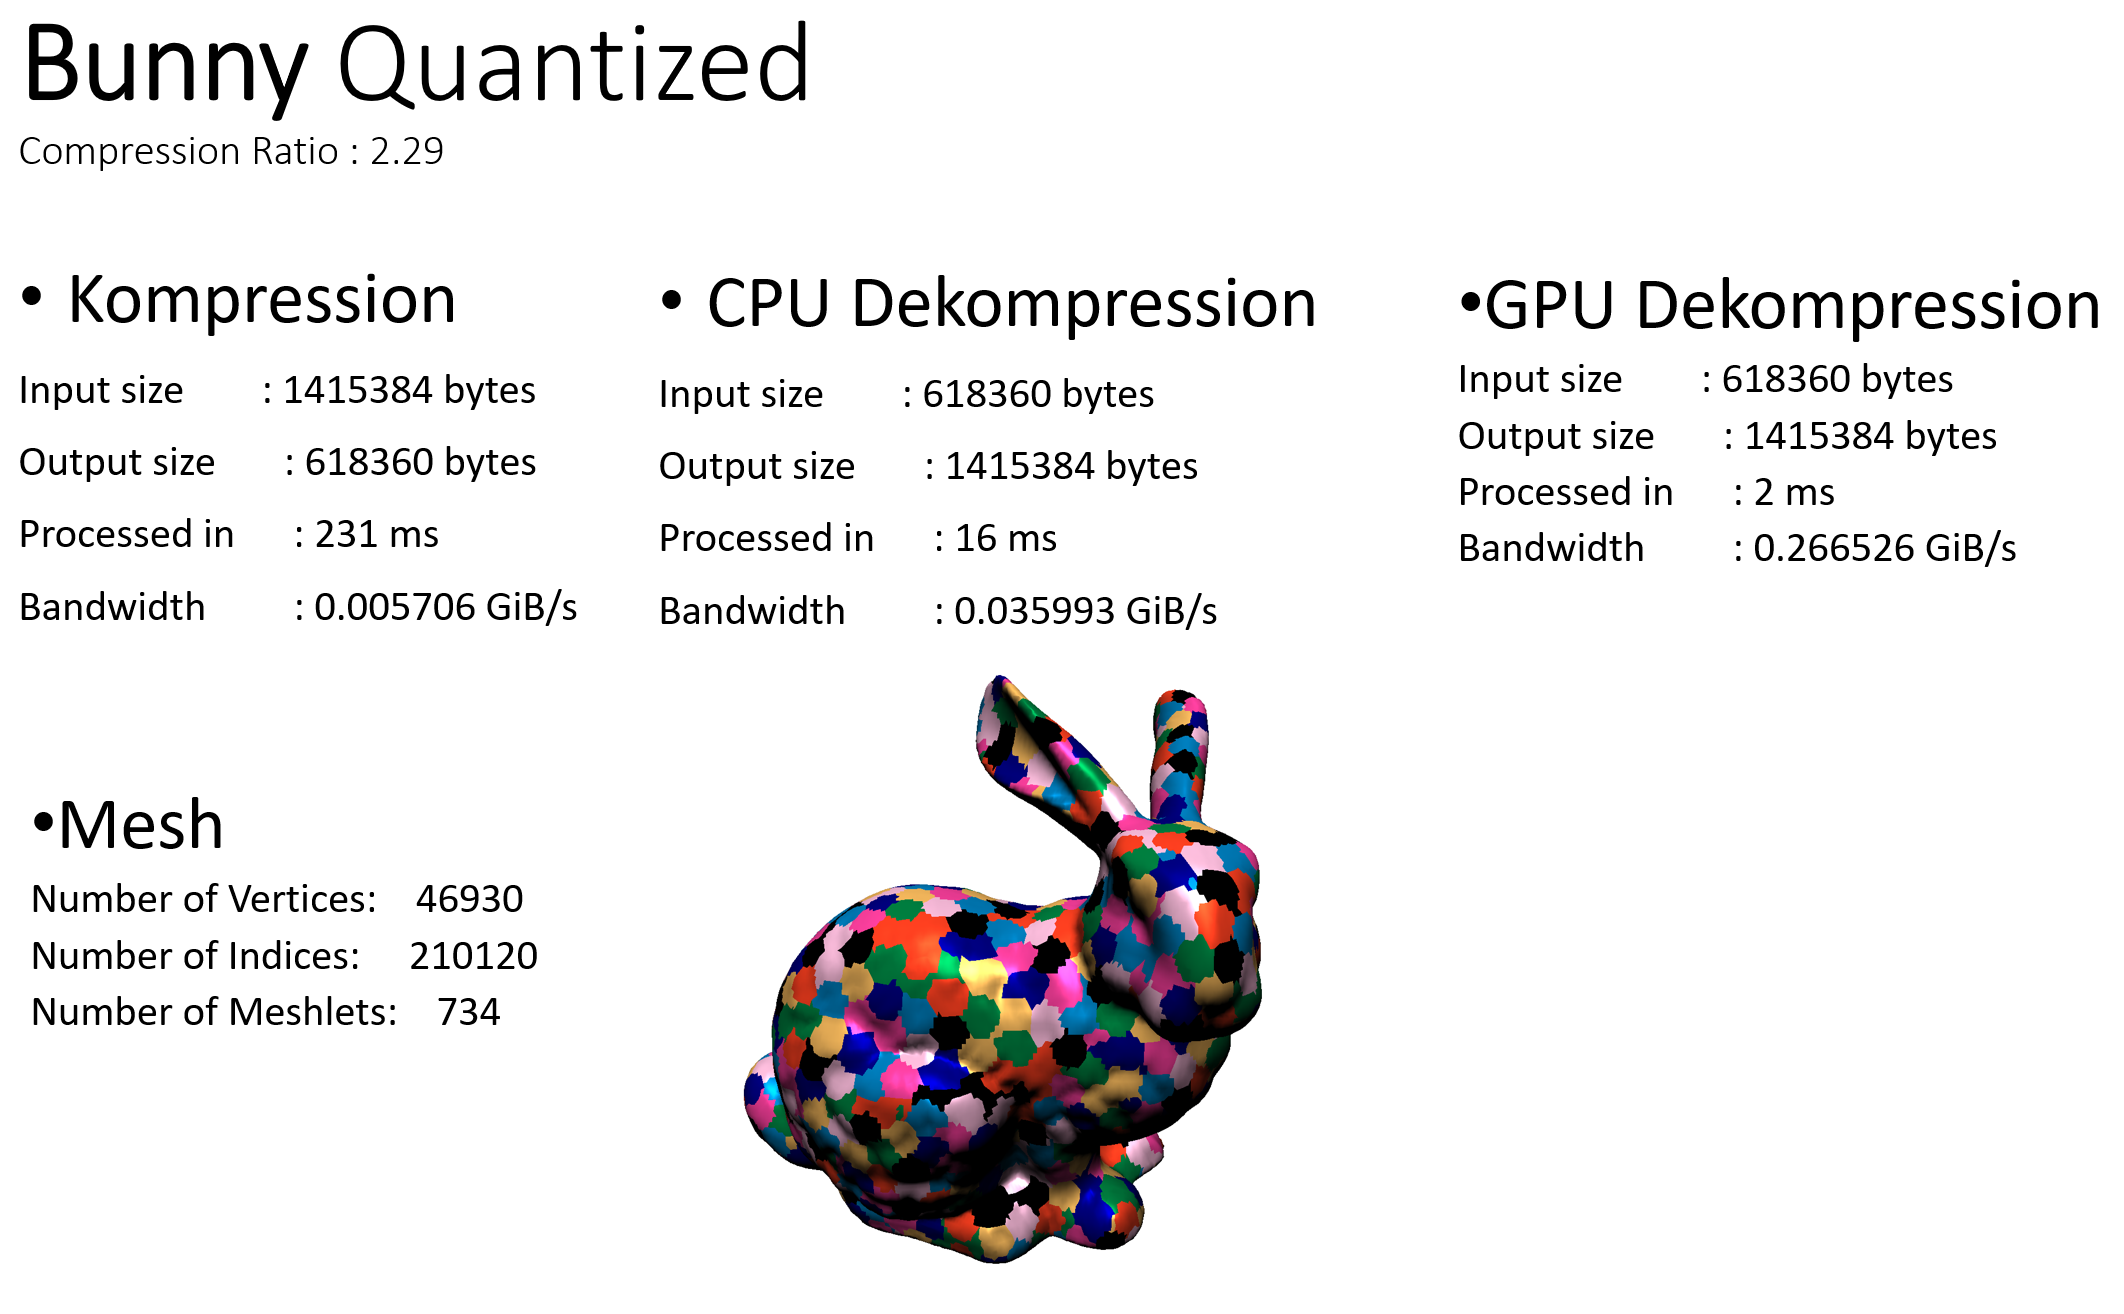
\includegraphics[scale=0.28]{Bilder/ergebnisse_full/bunny_quantized.png}
\end{figure}
\begin{figure}[h]
  \centering  
  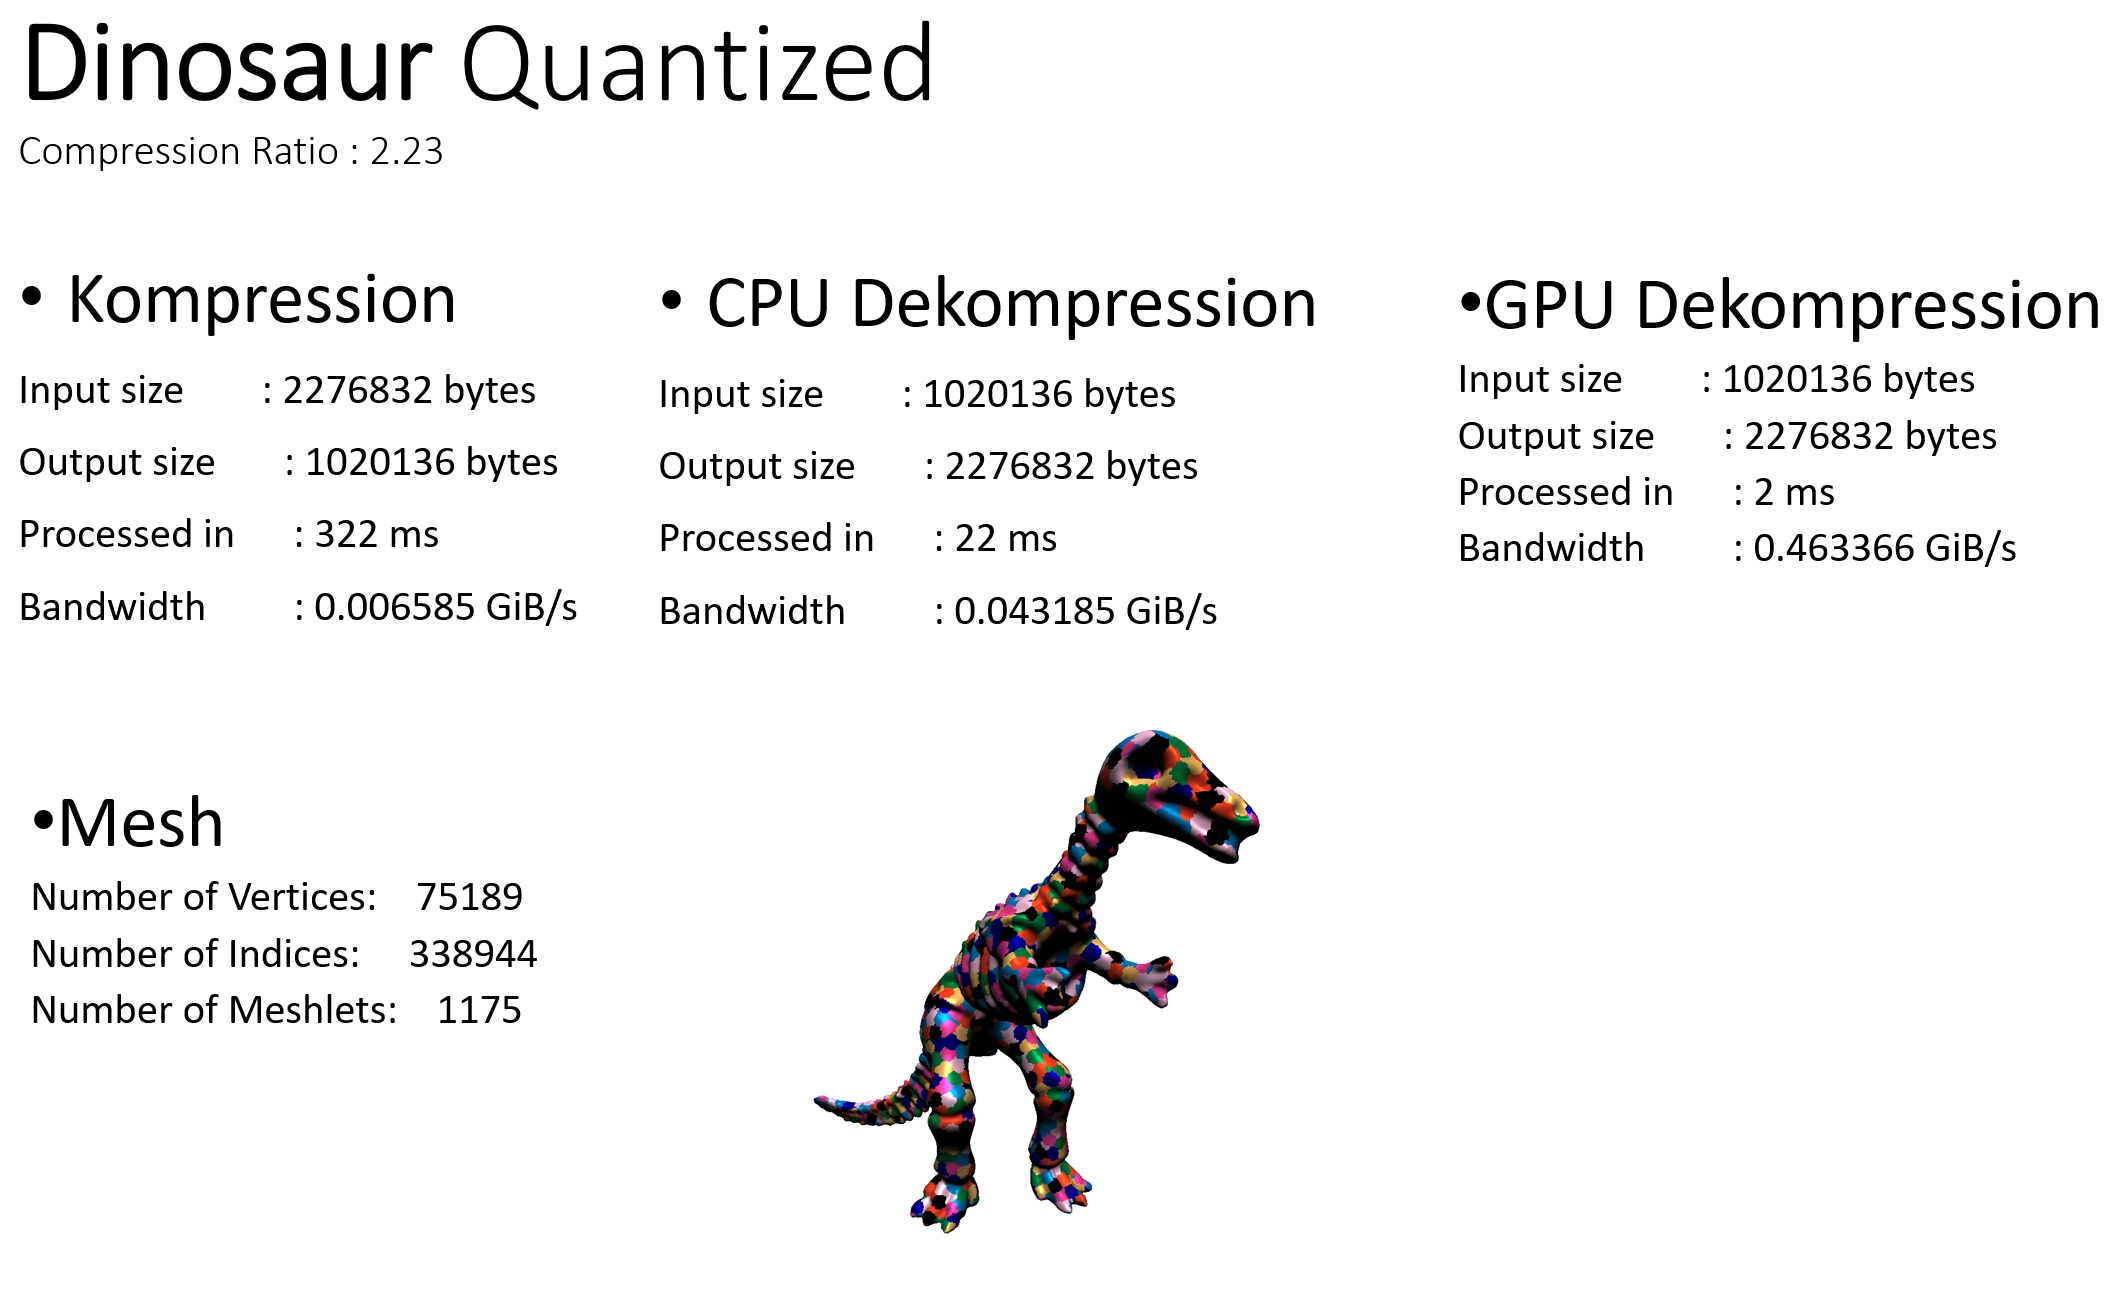
\includegraphics[scale=0.28]{Bilder/ergebnisse_full/dinosaur_quantized.png}
\end{figure}
\begin{figure}[h]
  \centering  
  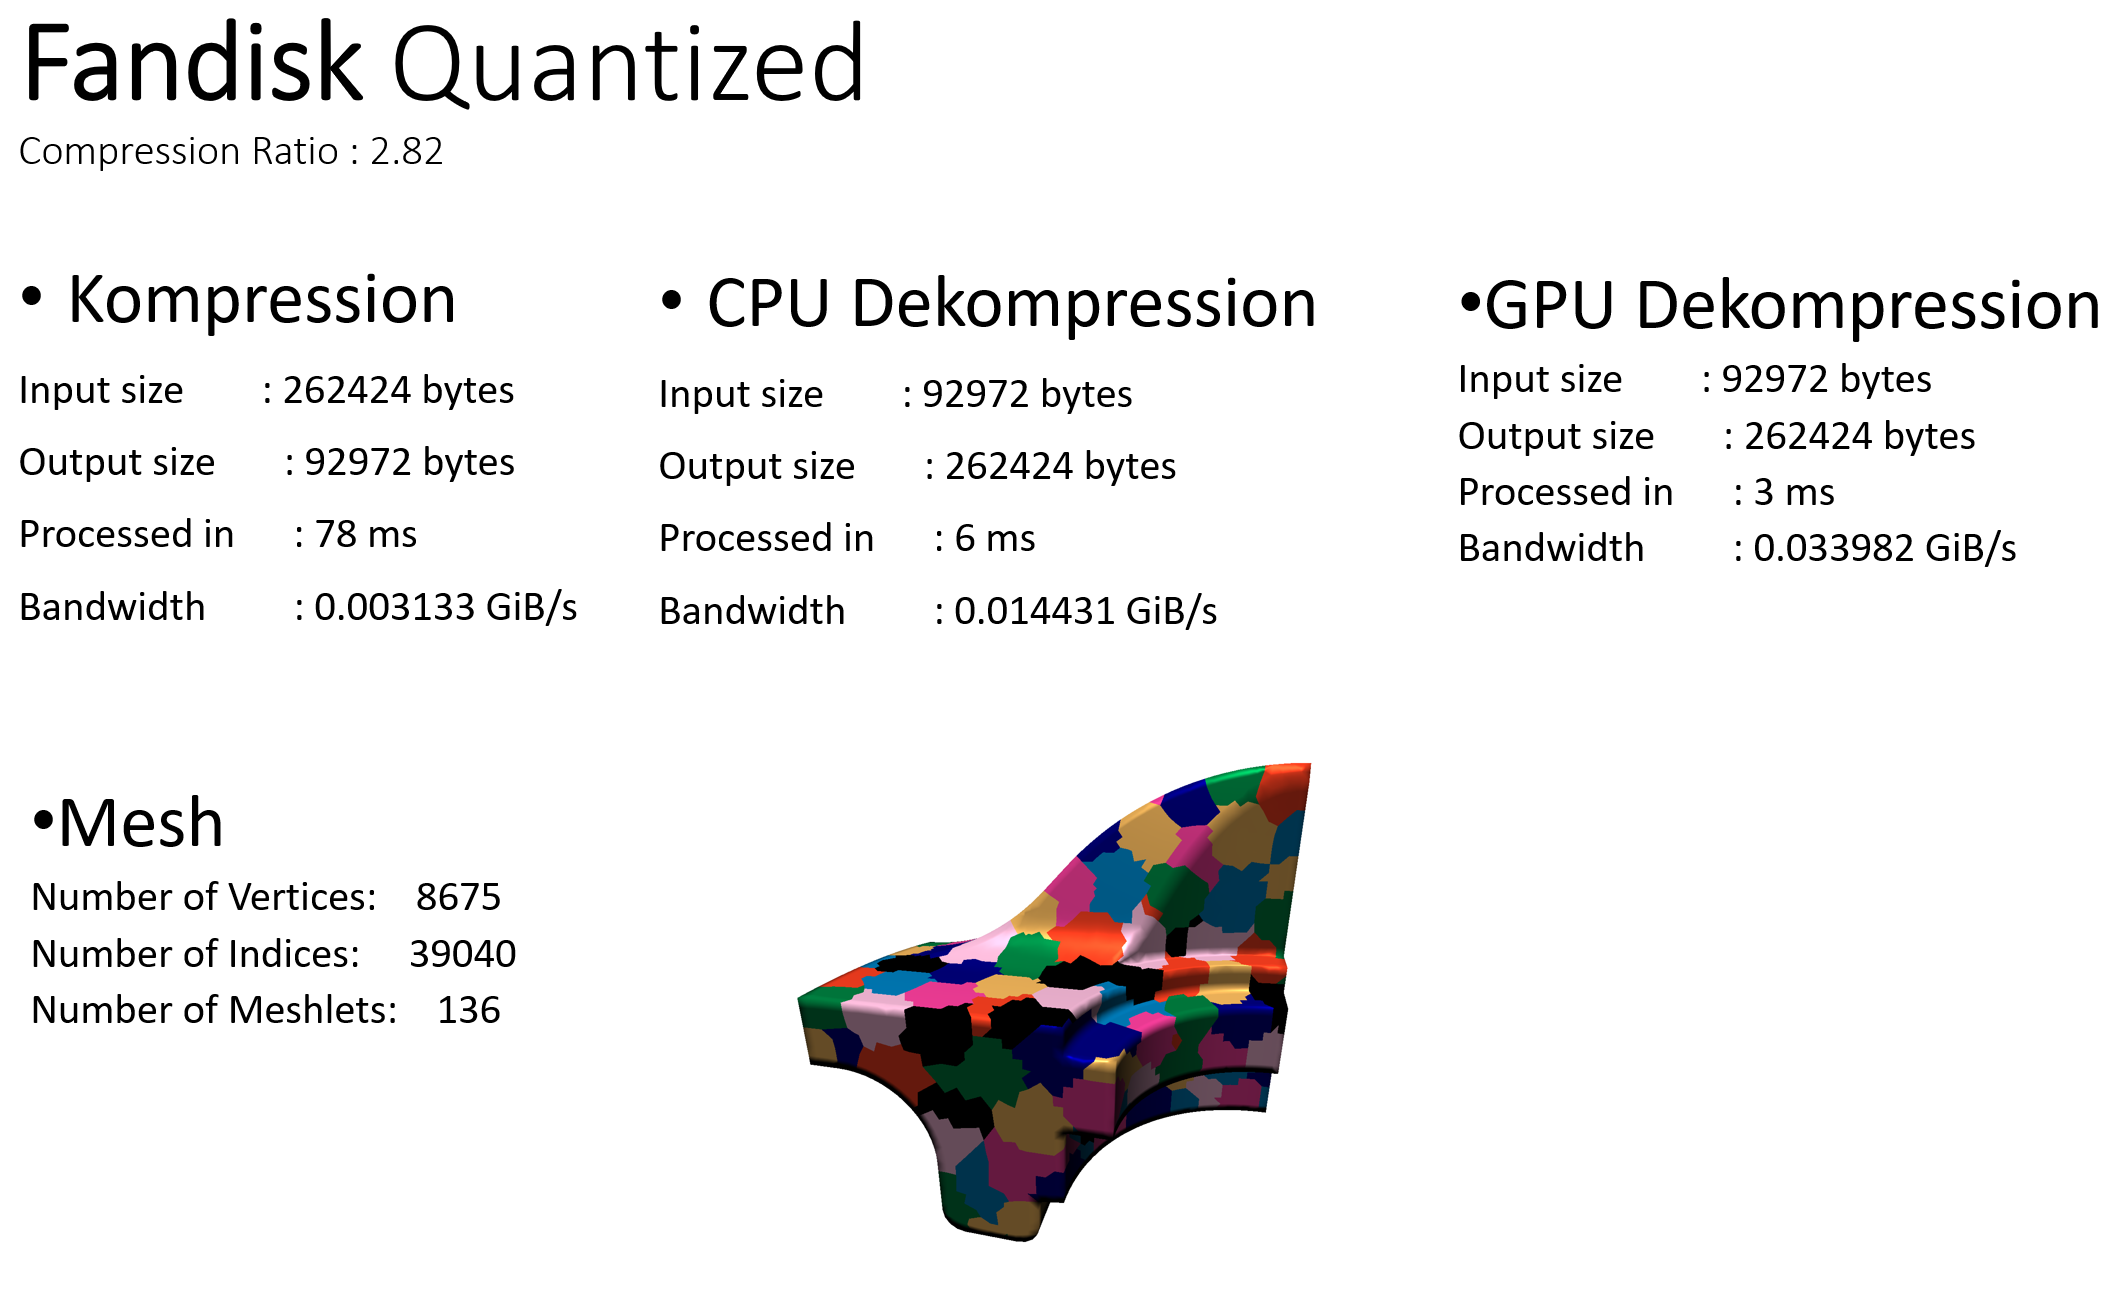
\includegraphics[scale=0.28]{Bilder/ergebnisse_full/fandisk_quantized.png}
\end{figure}
\begin{figure}[h]
  \centering  
  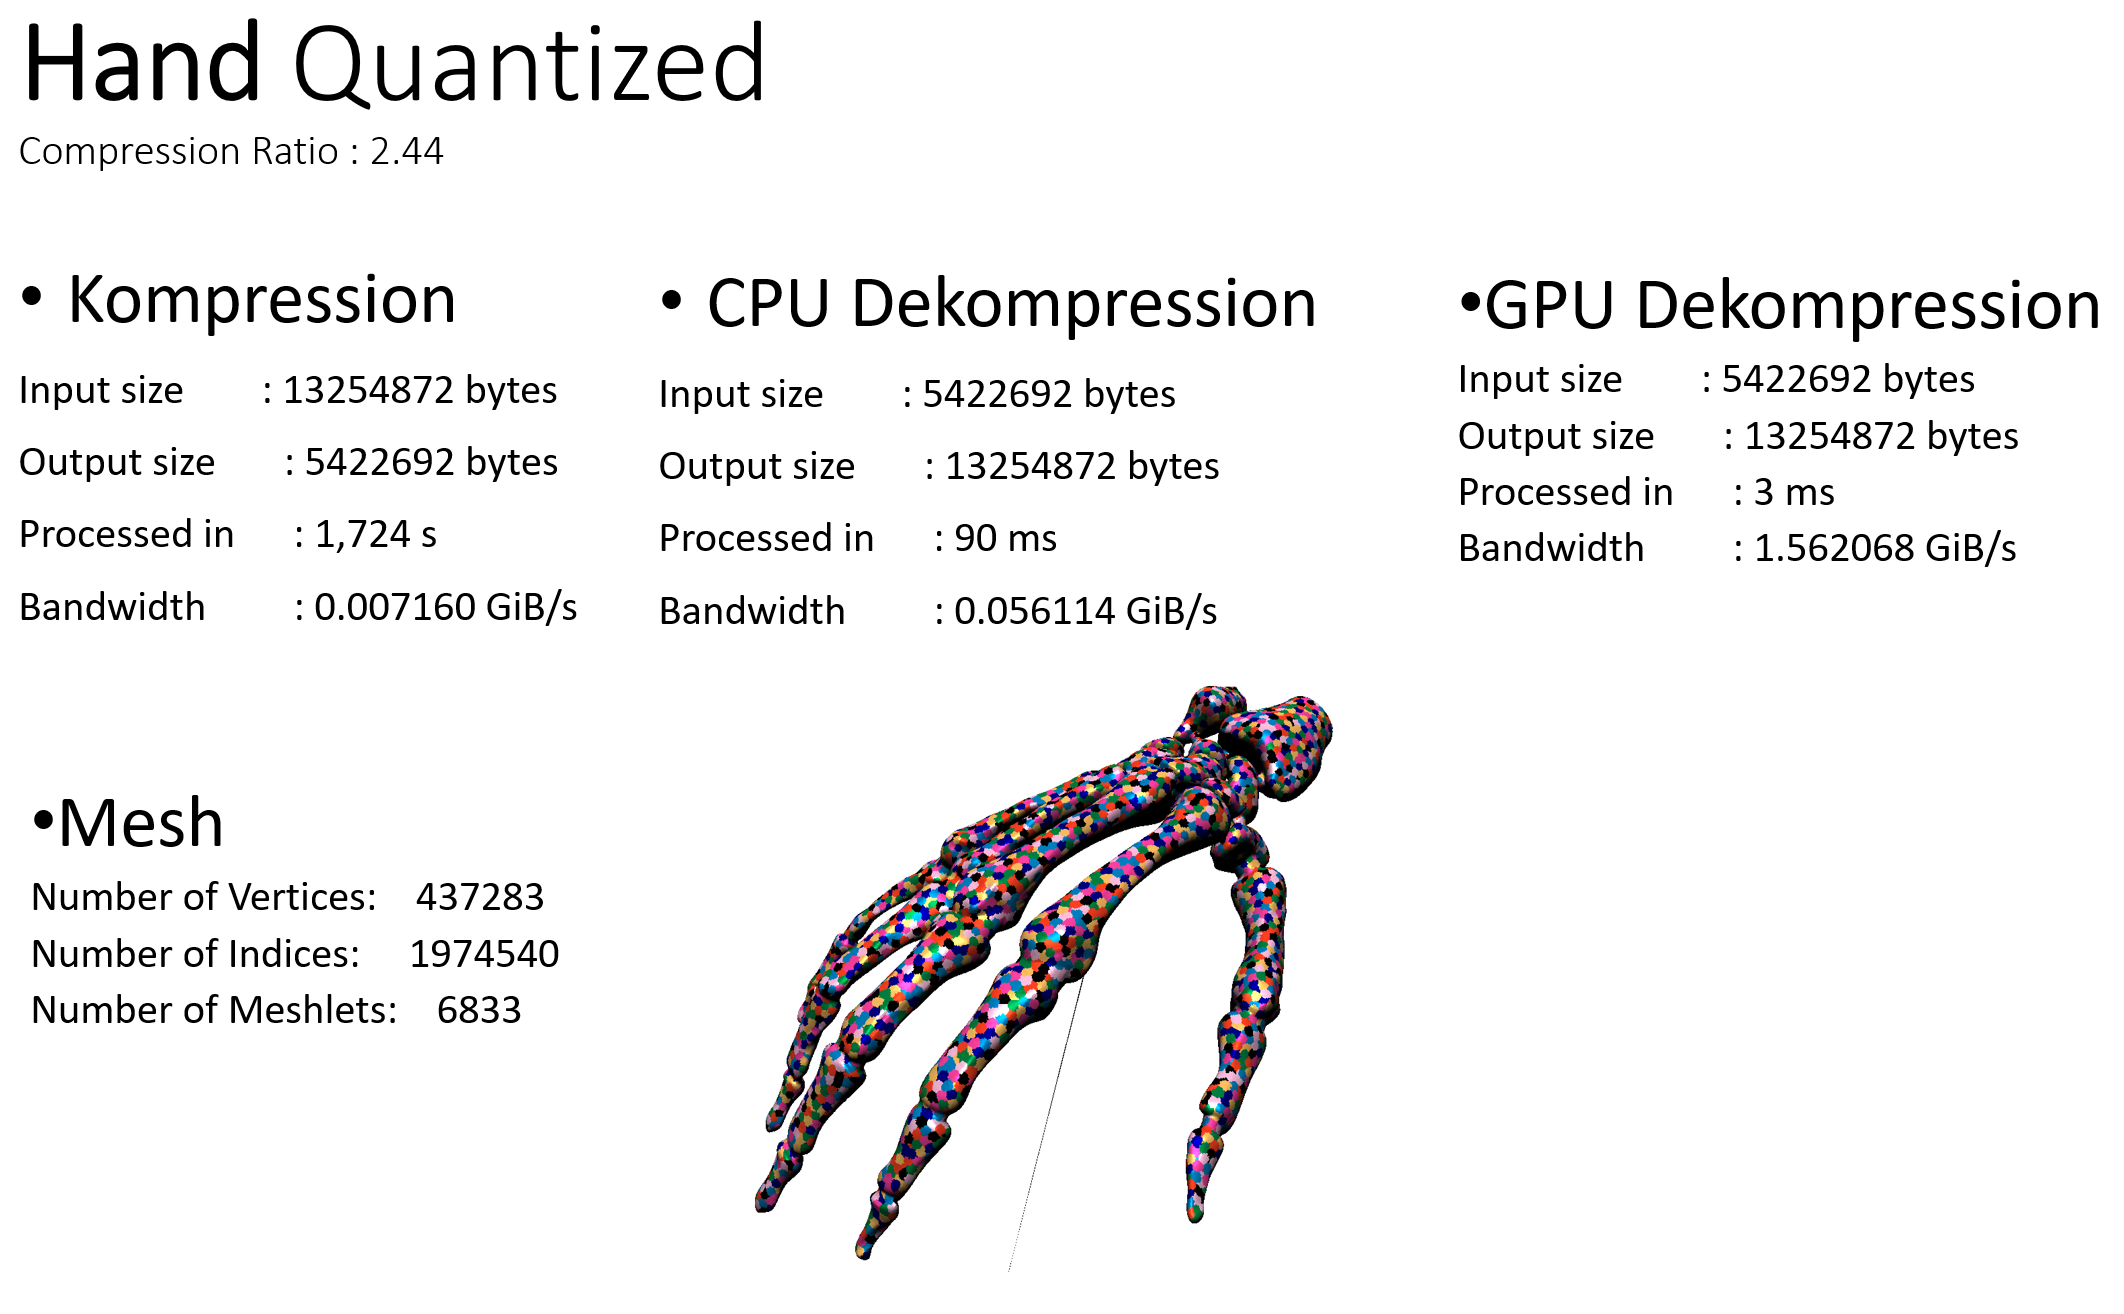
\includegraphics[scale=0.28]{Bilder/ergebnisse_full/hand_quantized.png}
\end{figure}
\begin{figure}[h]
  \centering  
  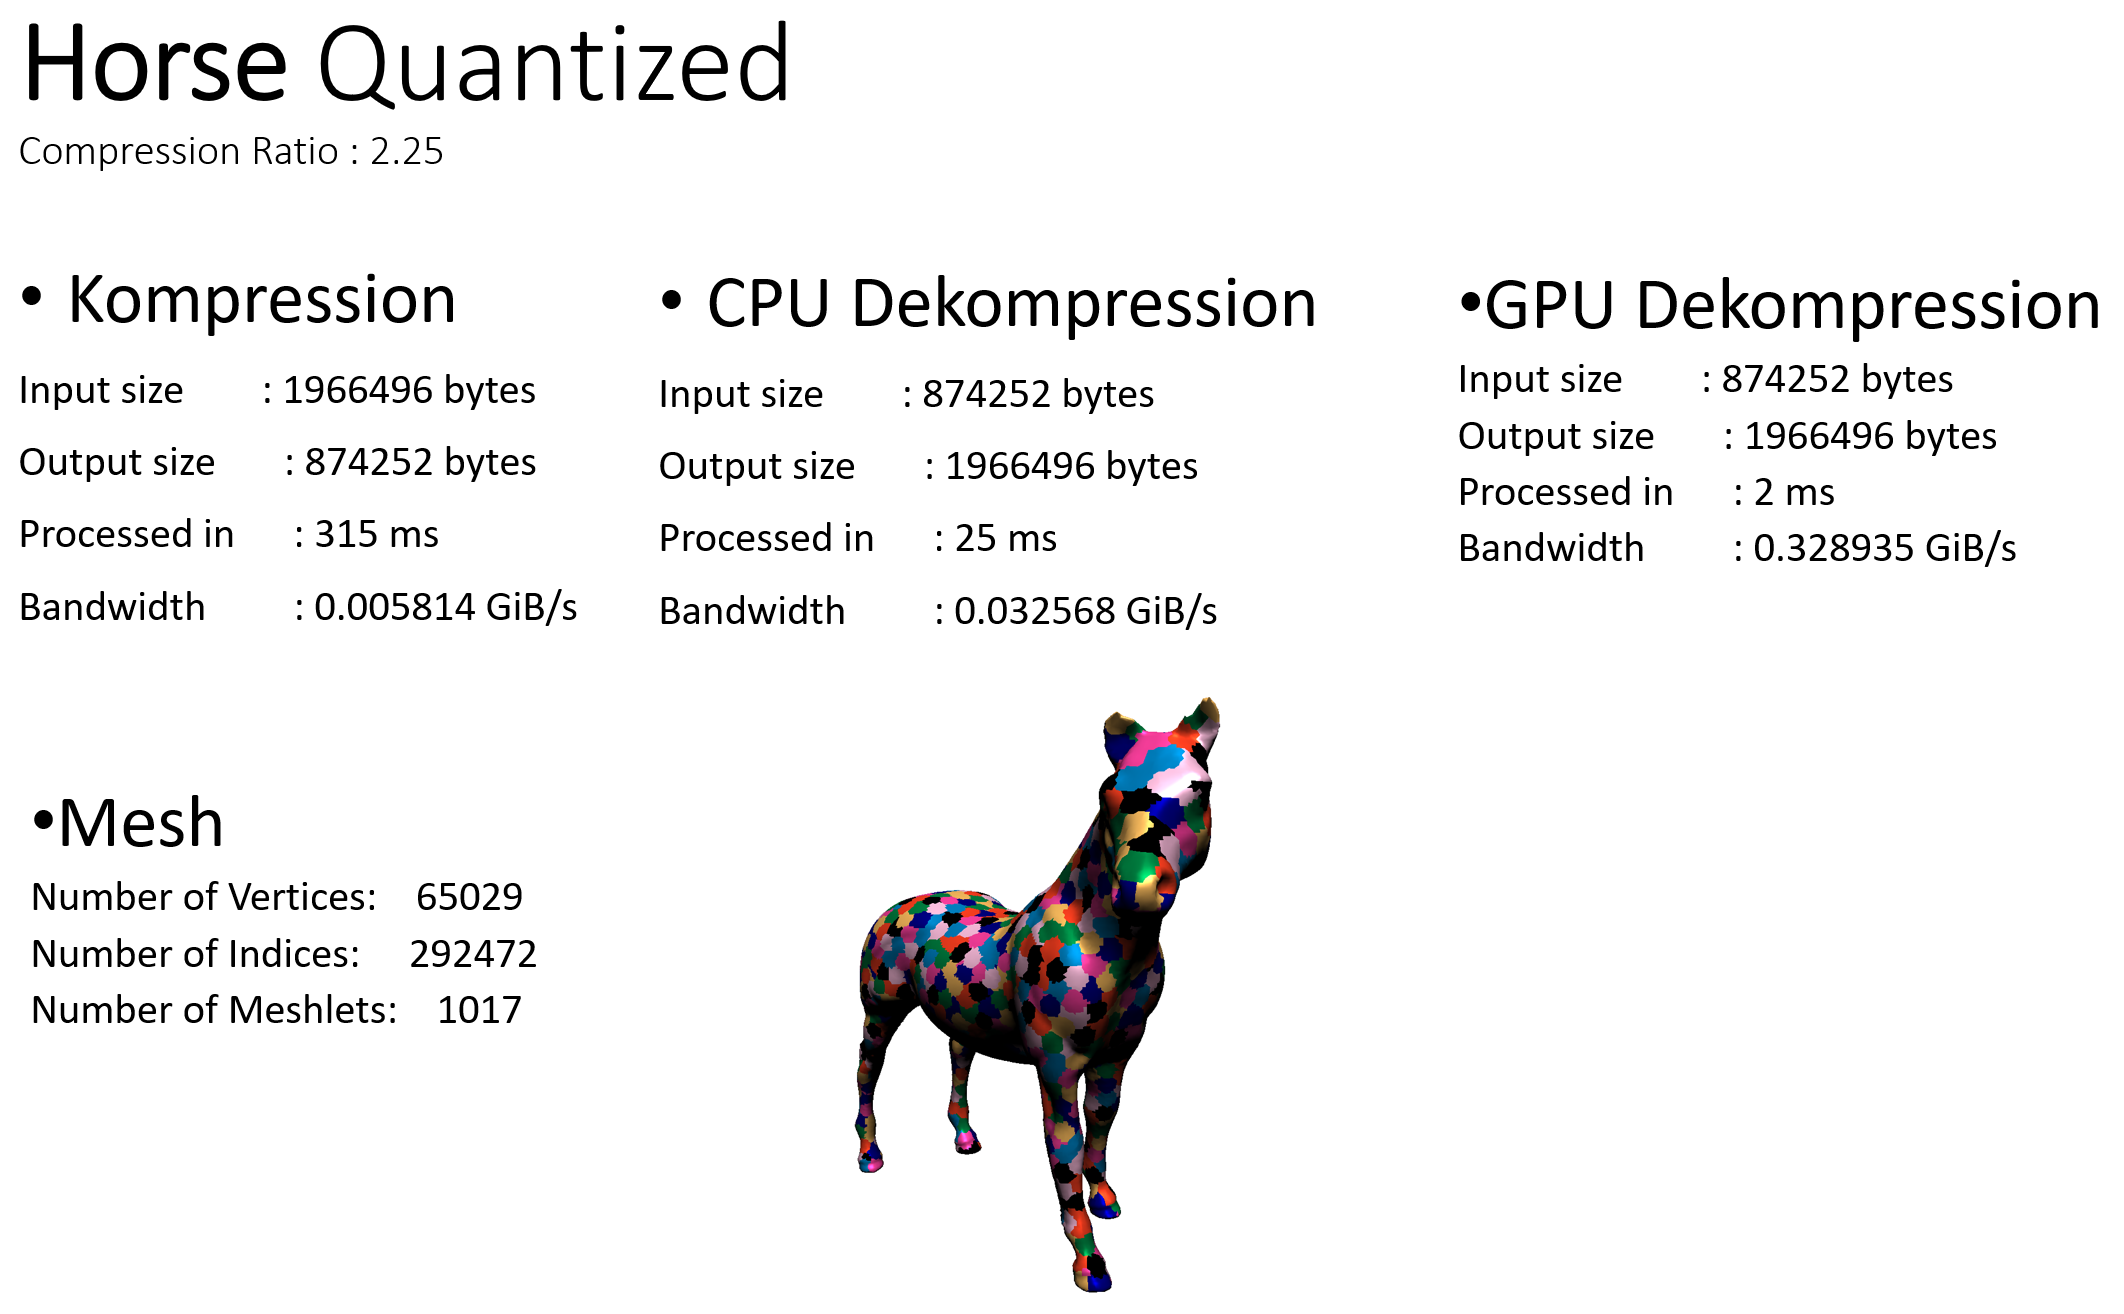
\includegraphics[scale=0.28]{Bilder/ergebnisse_full/horse_quantized.png}
\end{figure}
\begin{figure}[h]
  \centering  
  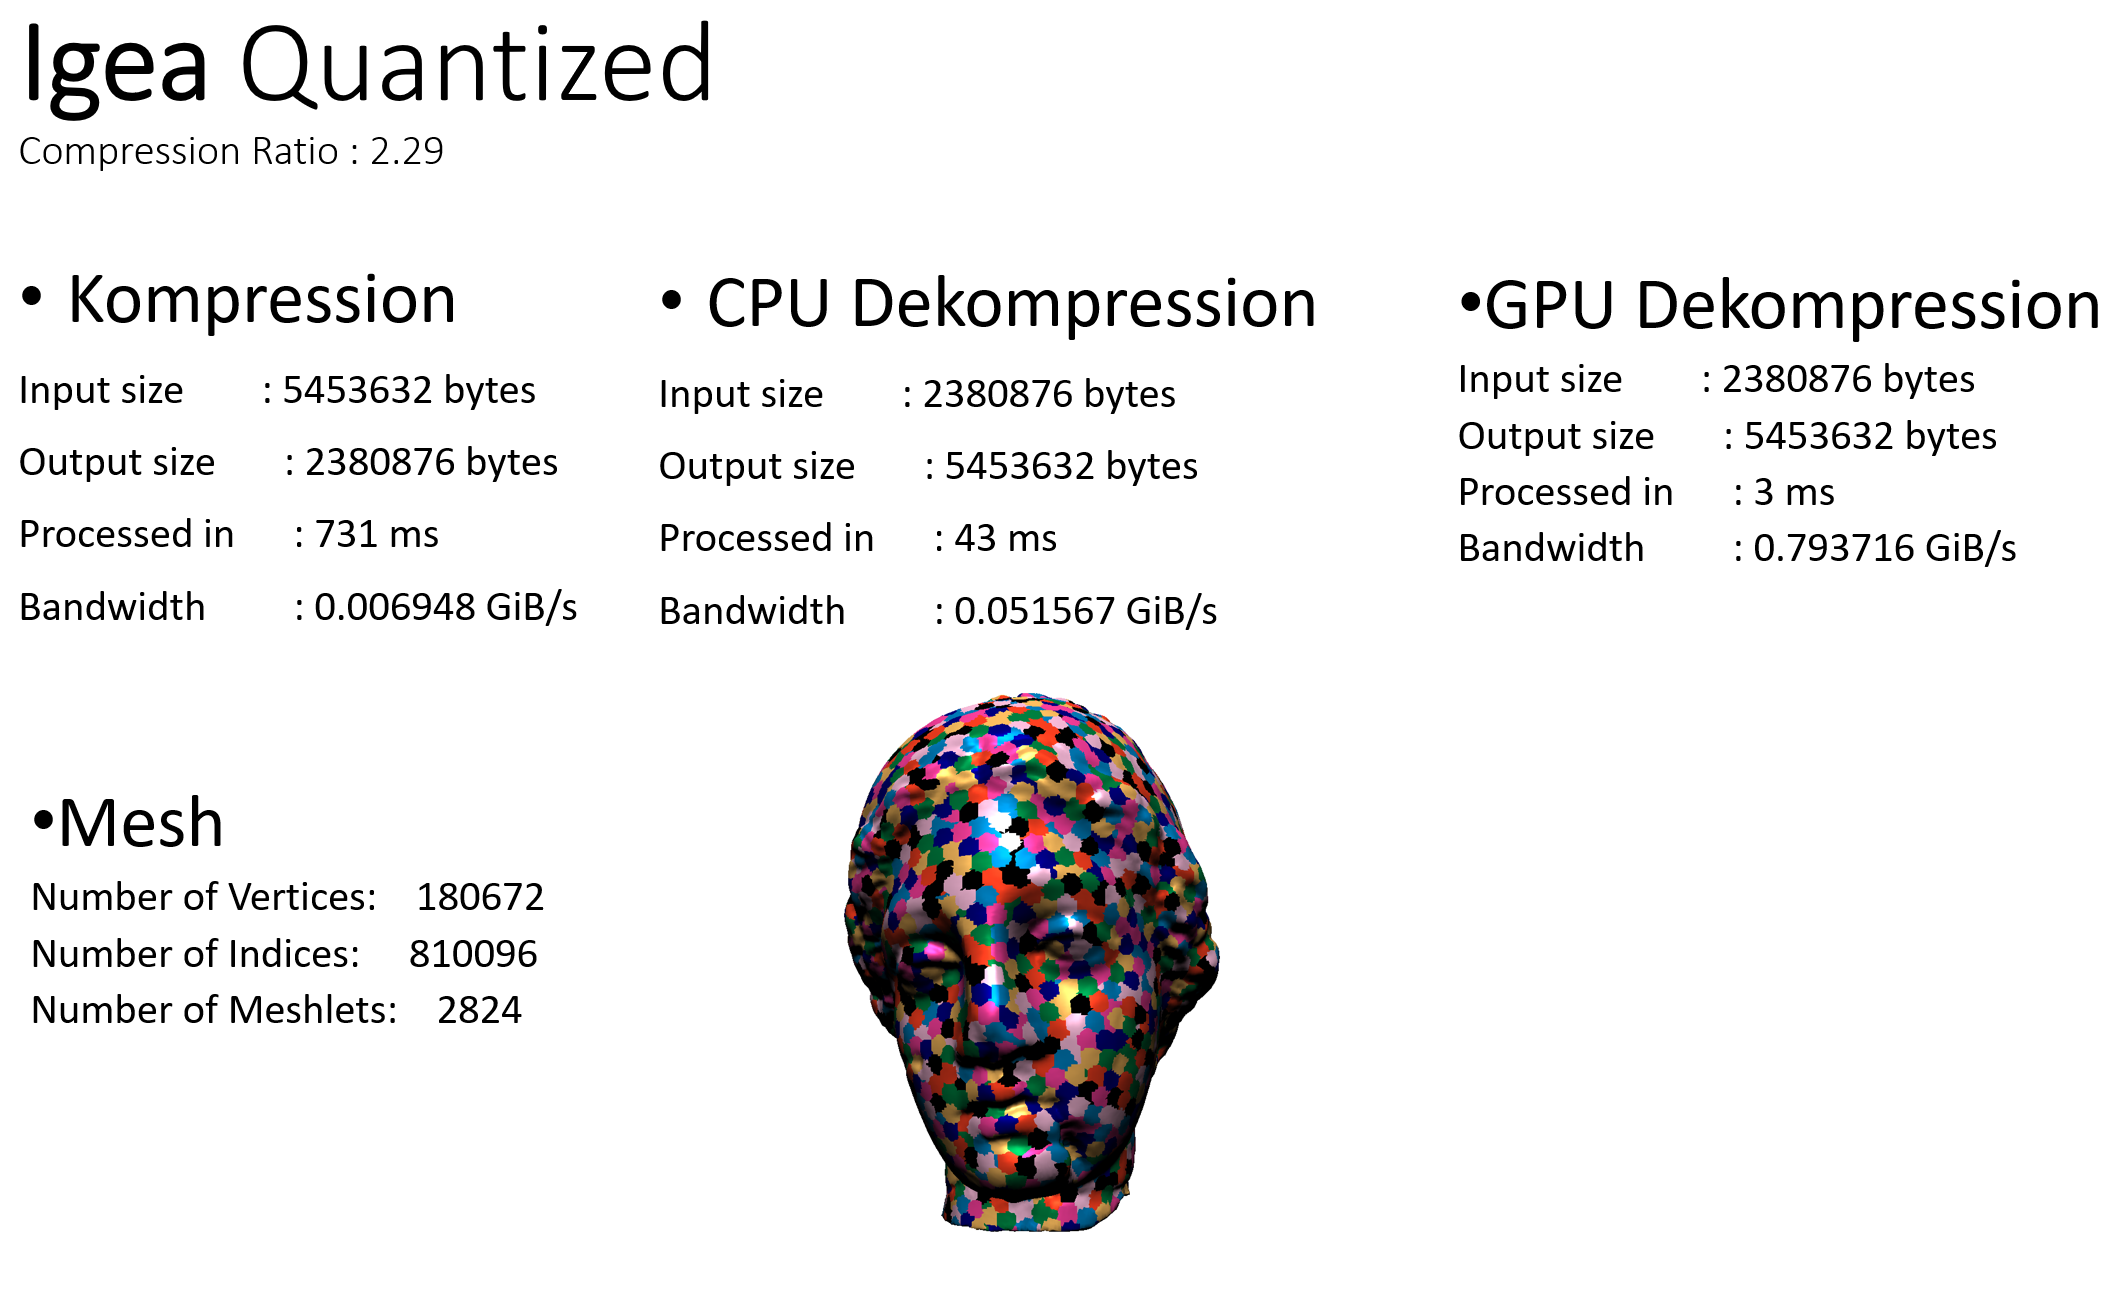
\includegraphics[scale=0.28]{Bilder/ergebnisse_full/igea_quantized.png}
\end{figure}
\begin{figure}[h]
  \centering  
  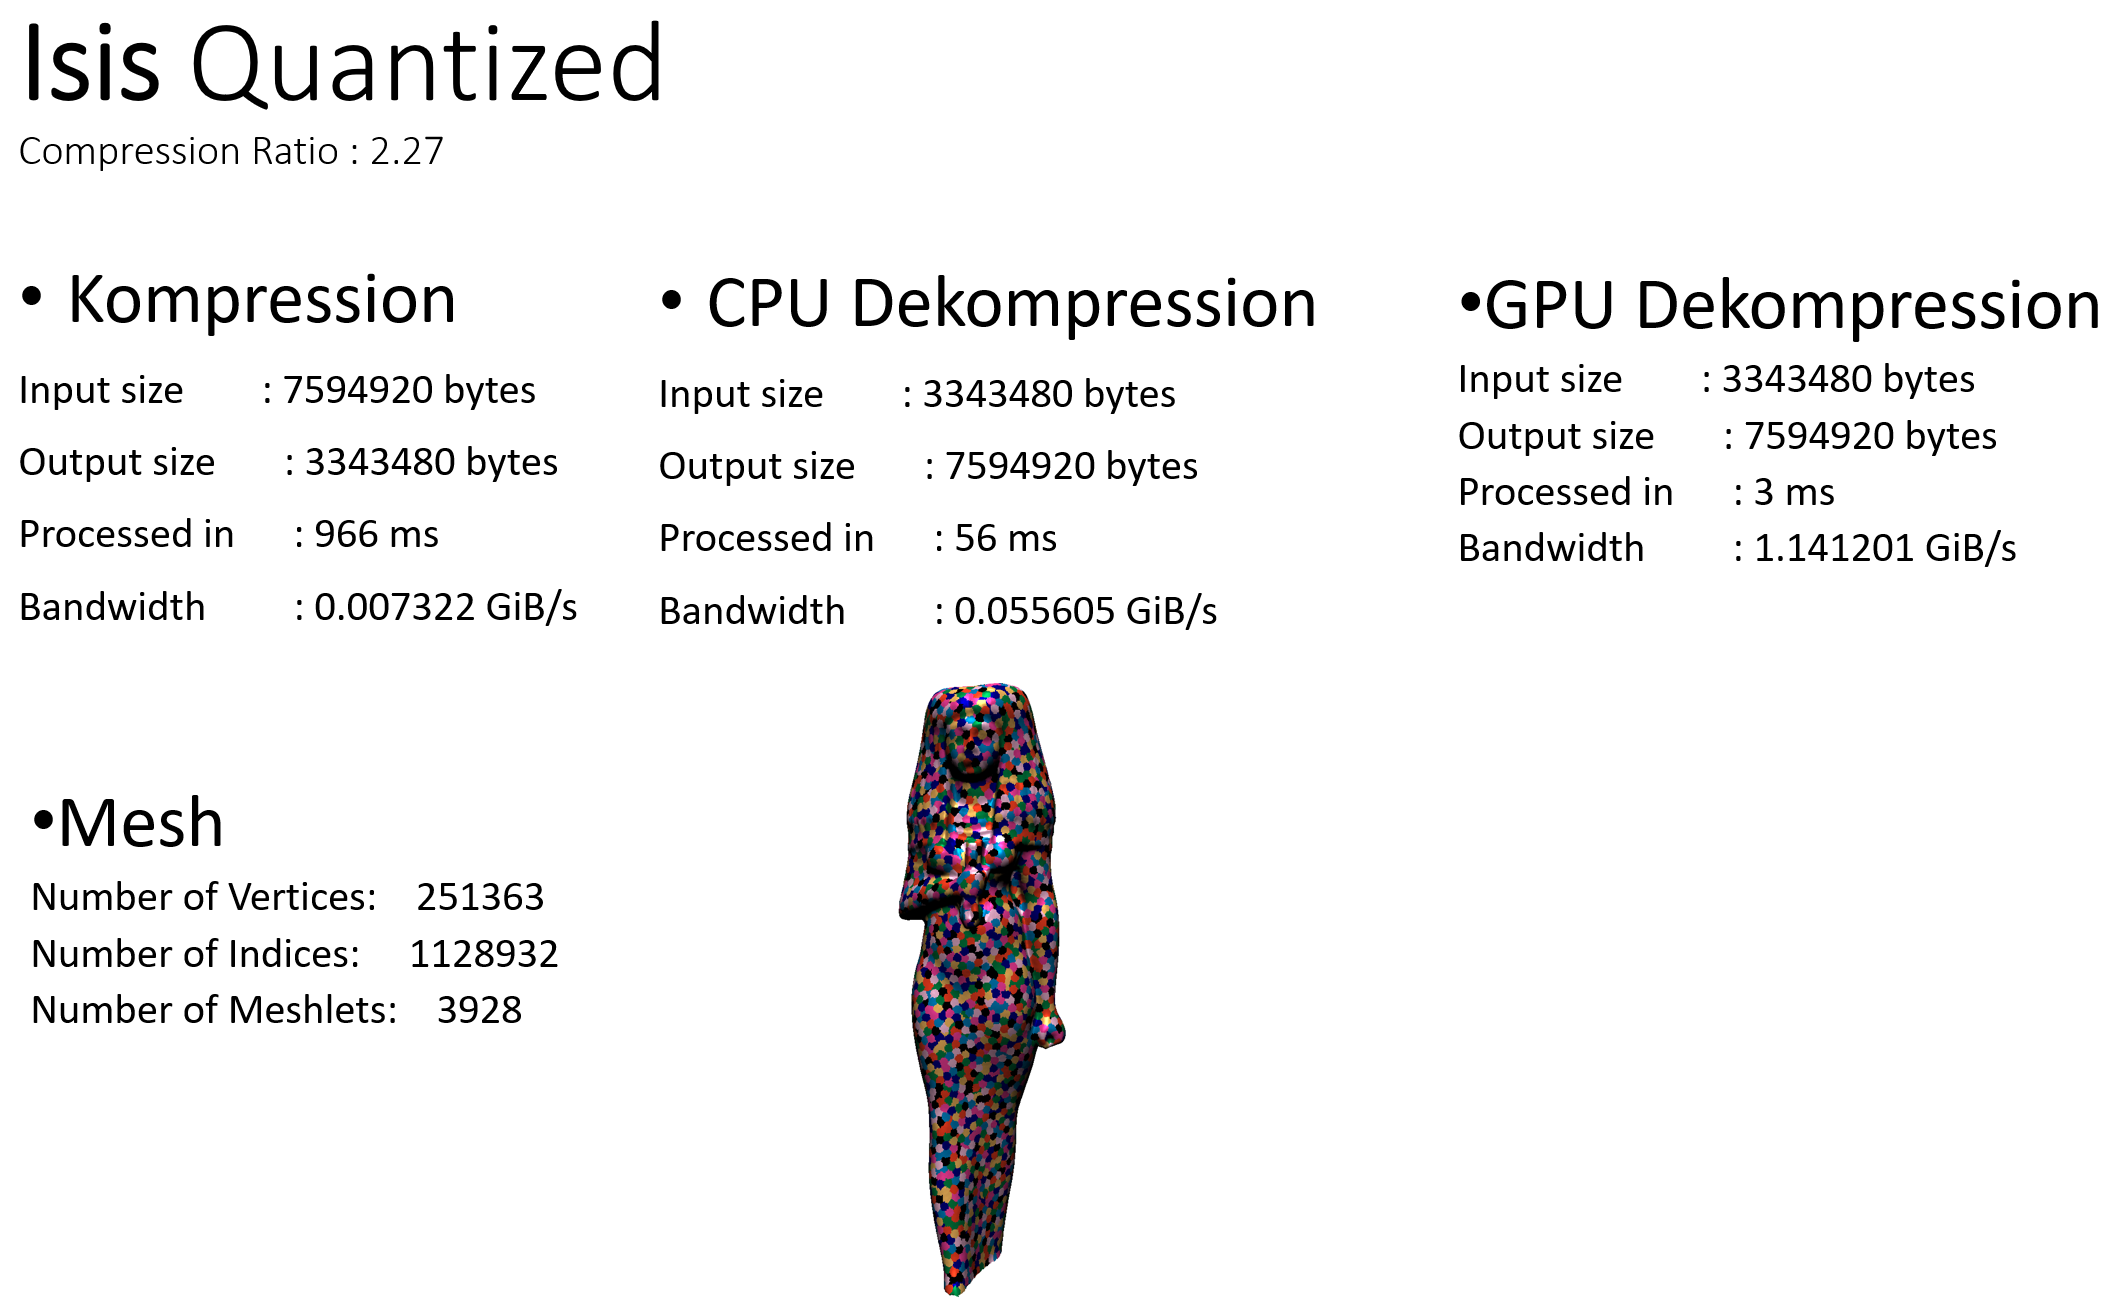
\includegraphics[scale=0.28]{Bilder/ergebnisse_full/isis_quantized.png}
\end{figure}
\begin{figure}[h]
  \centering  
  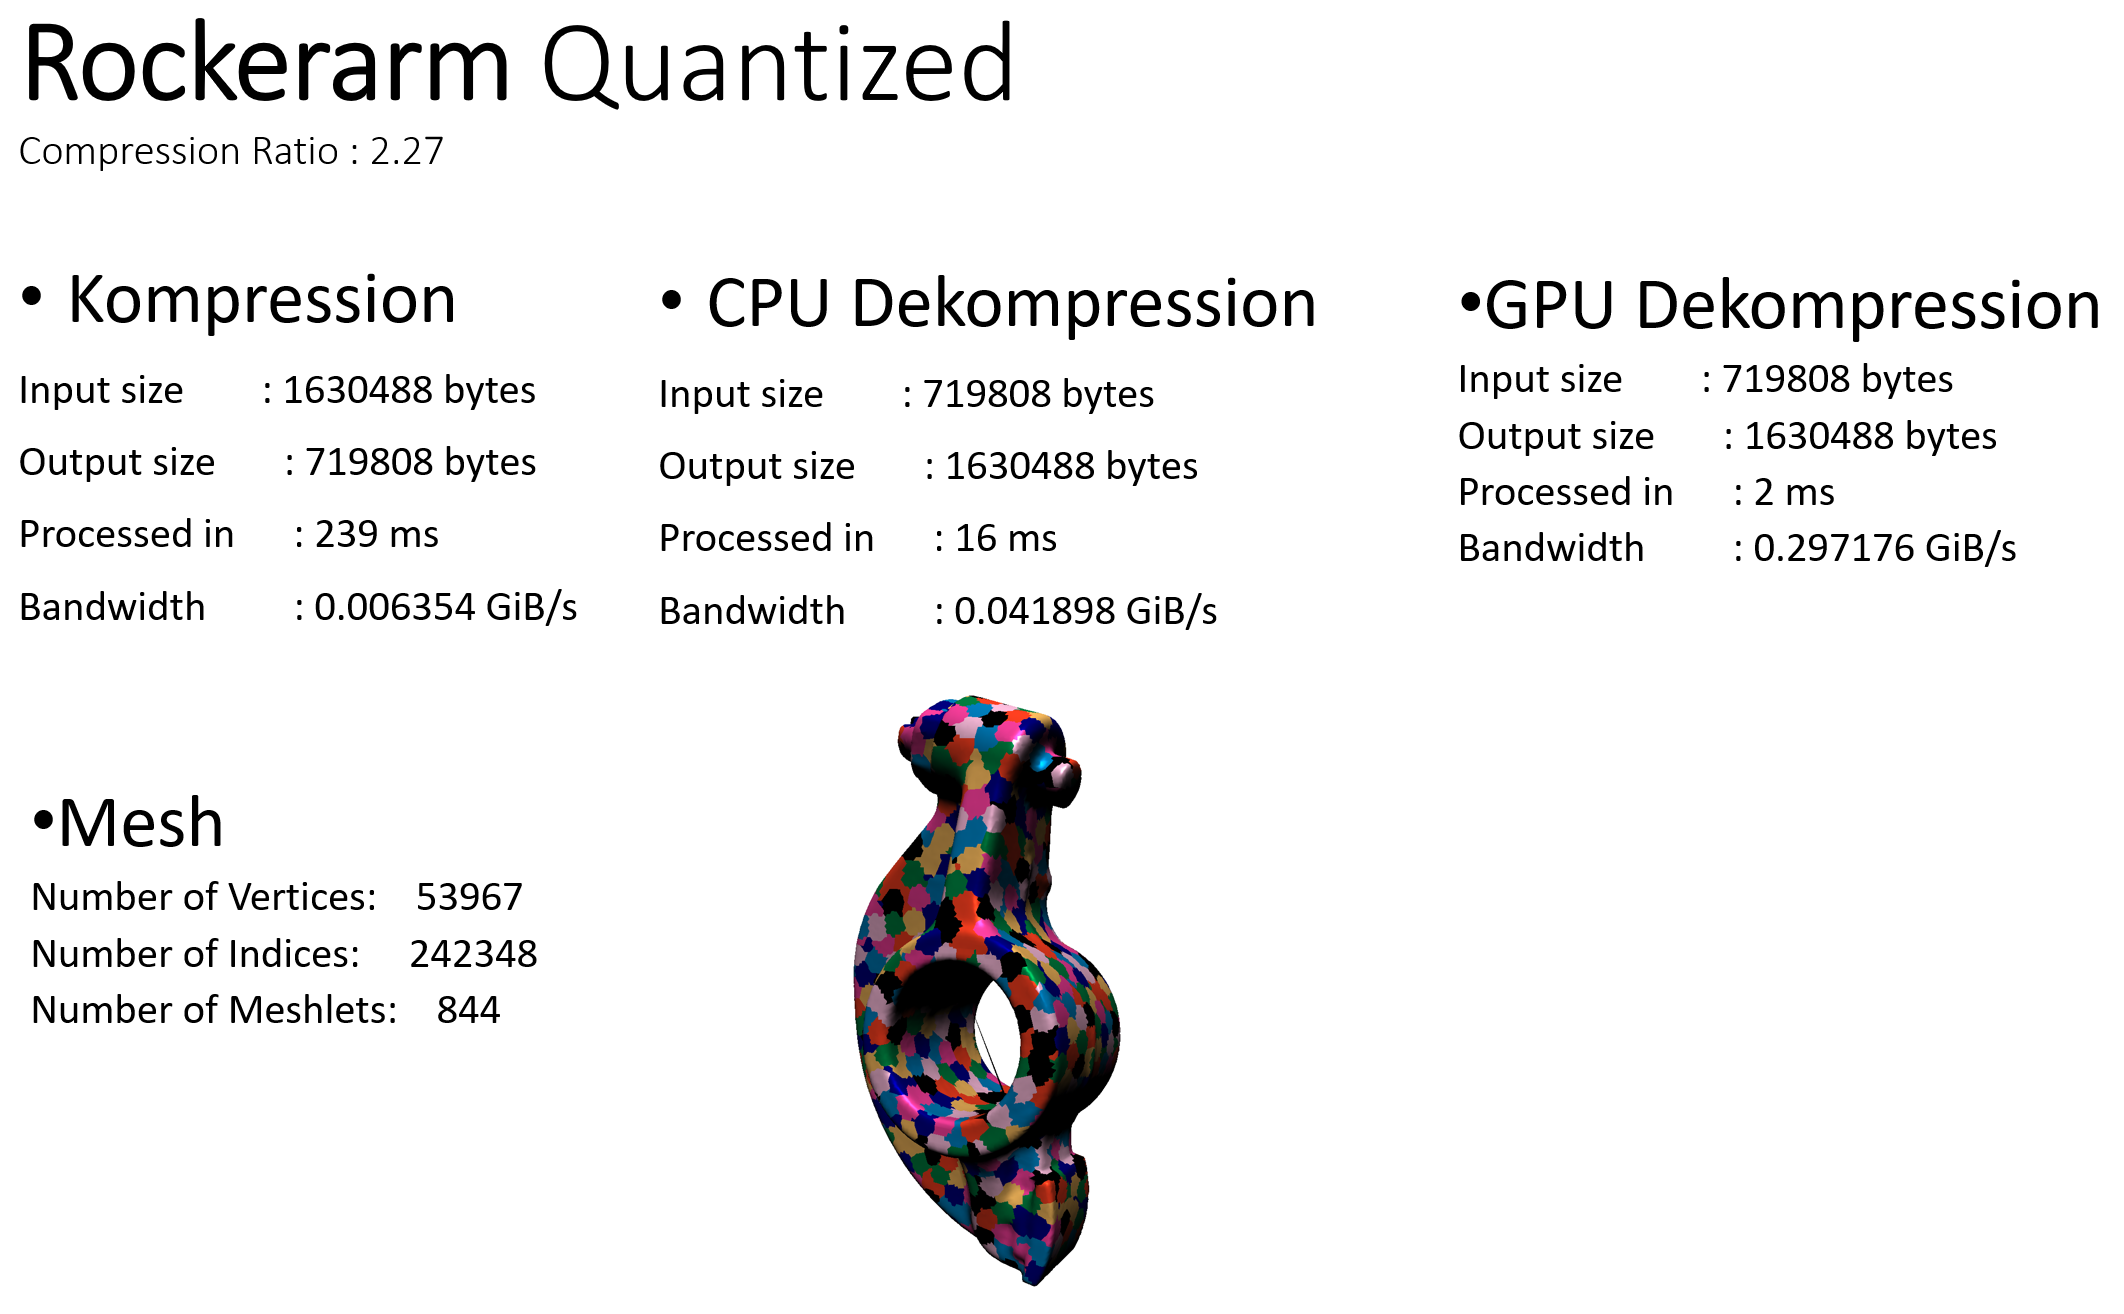
\includegraphics[scale=0.28]{Bilder/ergebnisse_full/rockerarm_quantized.png}
\end{figure}
\begin{figure}[h]
  \centering  
  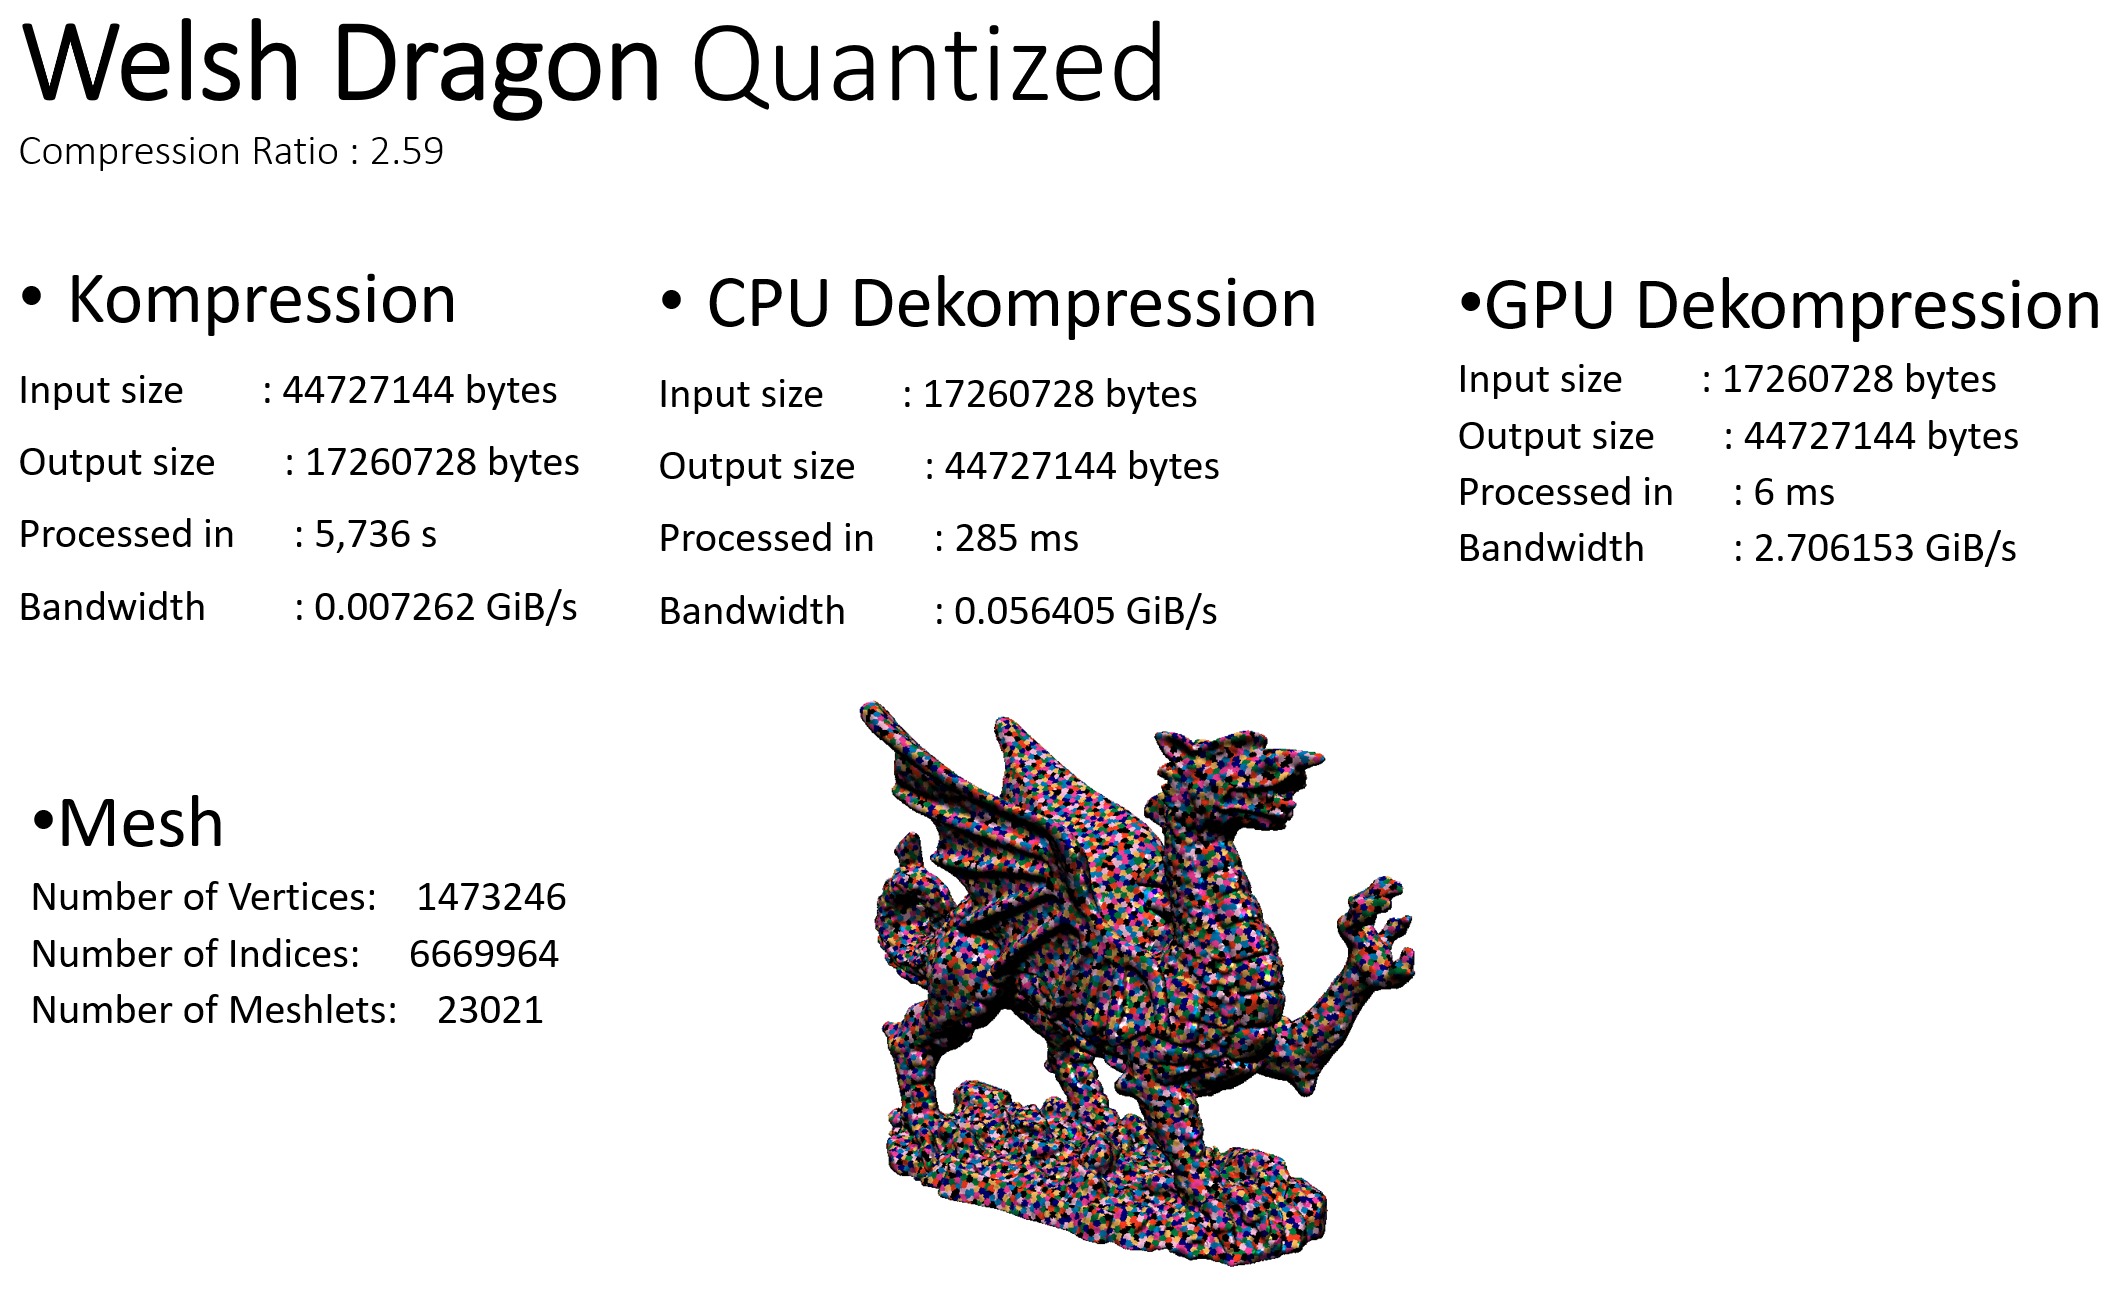
\includegraphics[scale=0.28]{Bilder/ergebnisse_full/welshdragon_quantized.png}
\end{figure}
\begin{figure}[h]
  \centering  
  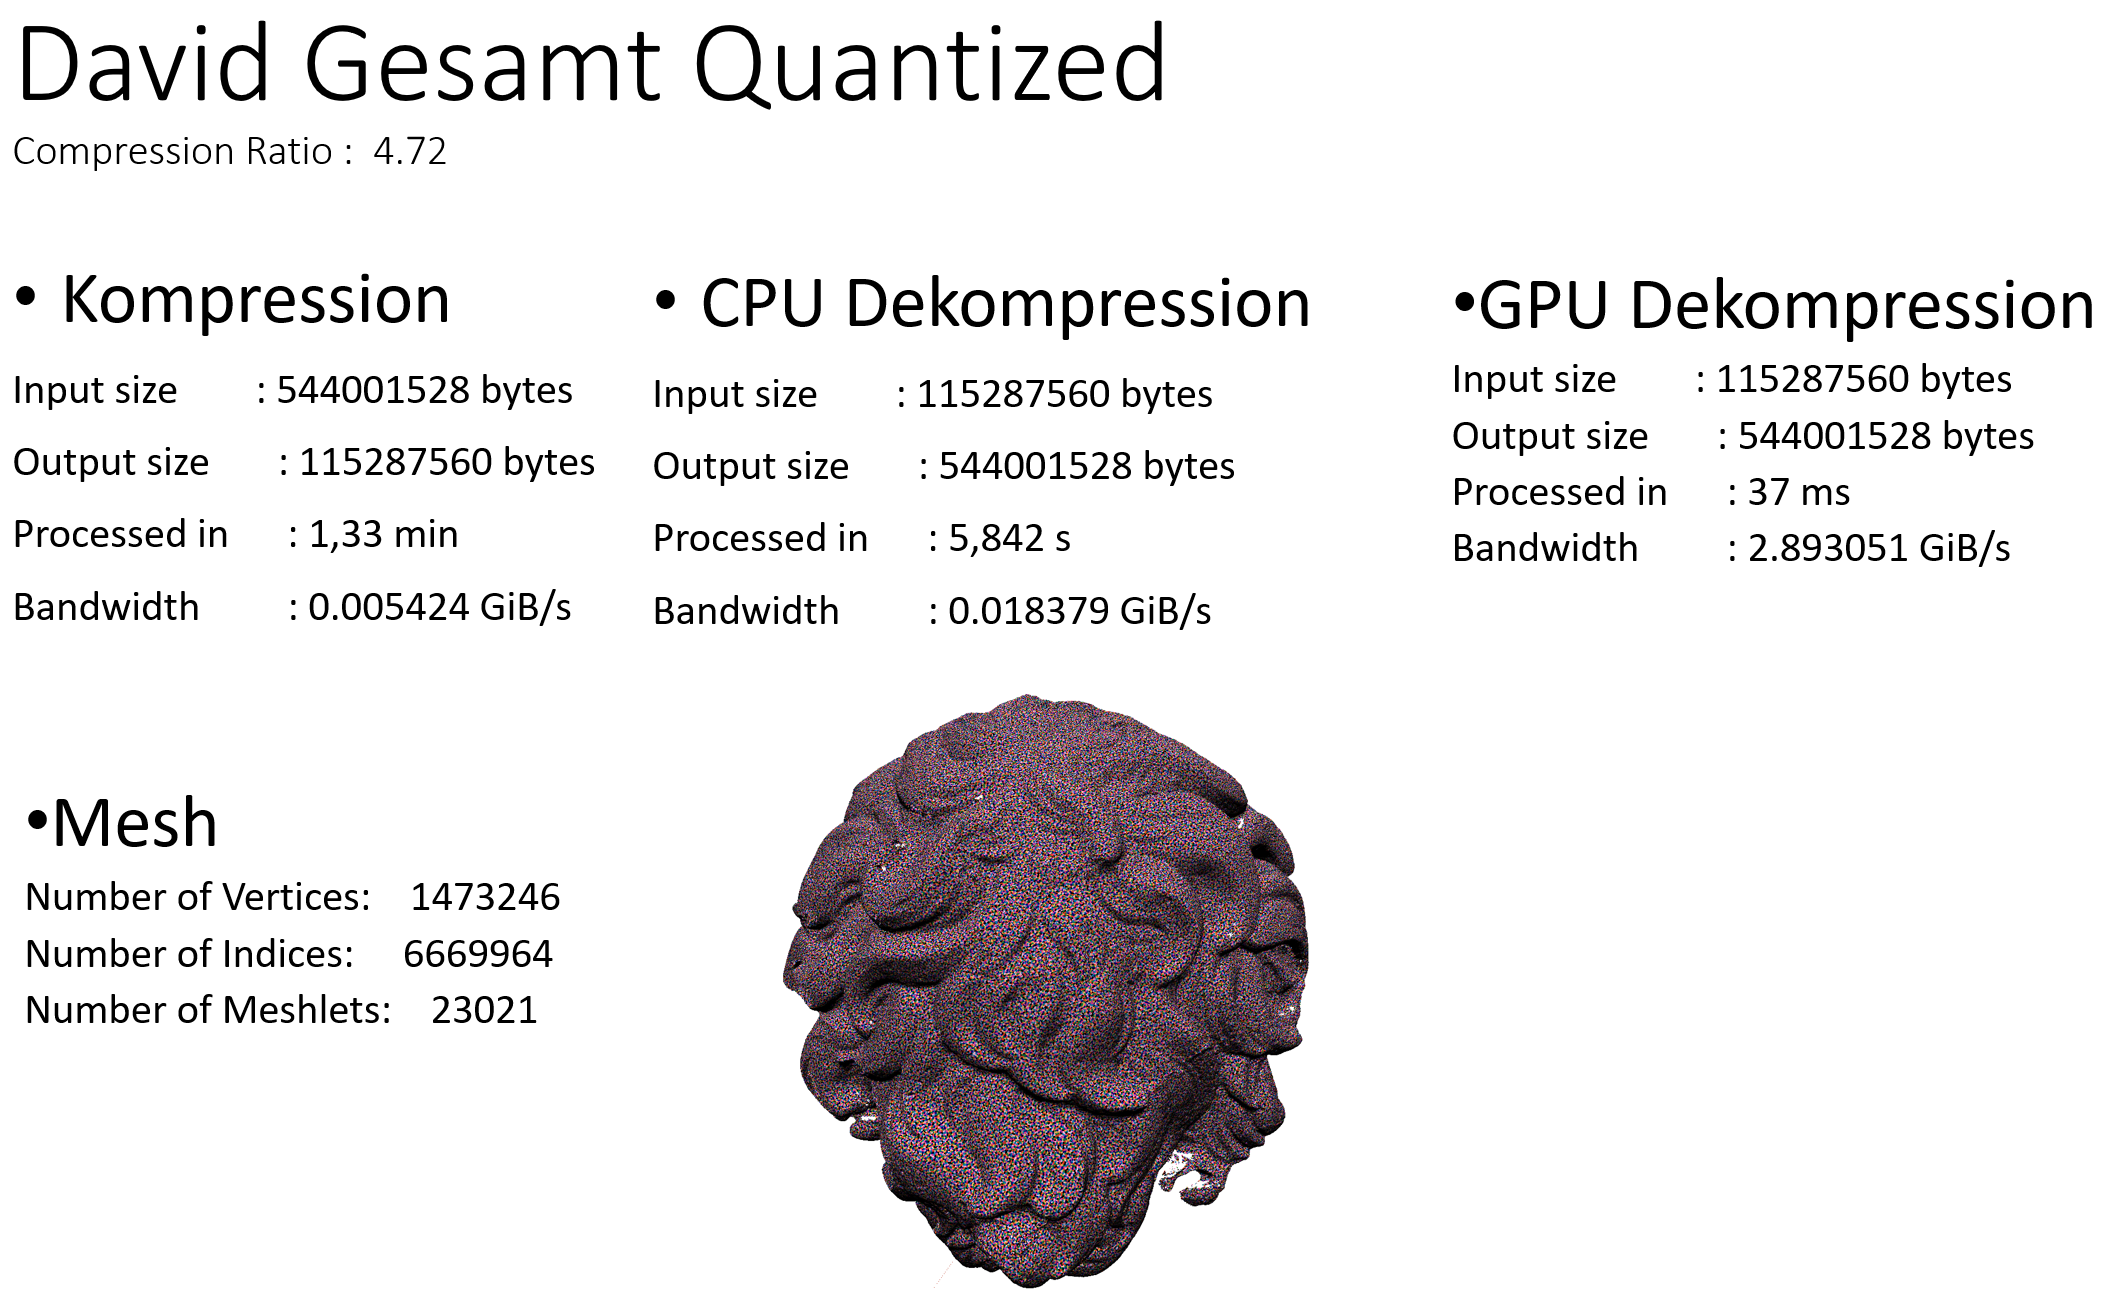
\includegraphics[scale=0.28]{Bilder/ergebnisse_full/david_quantized.png}
\end{figure}
\clearpage
\subsection{Berechnung der verwendeten Prozentzahlen}
\begin{figure}[h]
  \centering  
  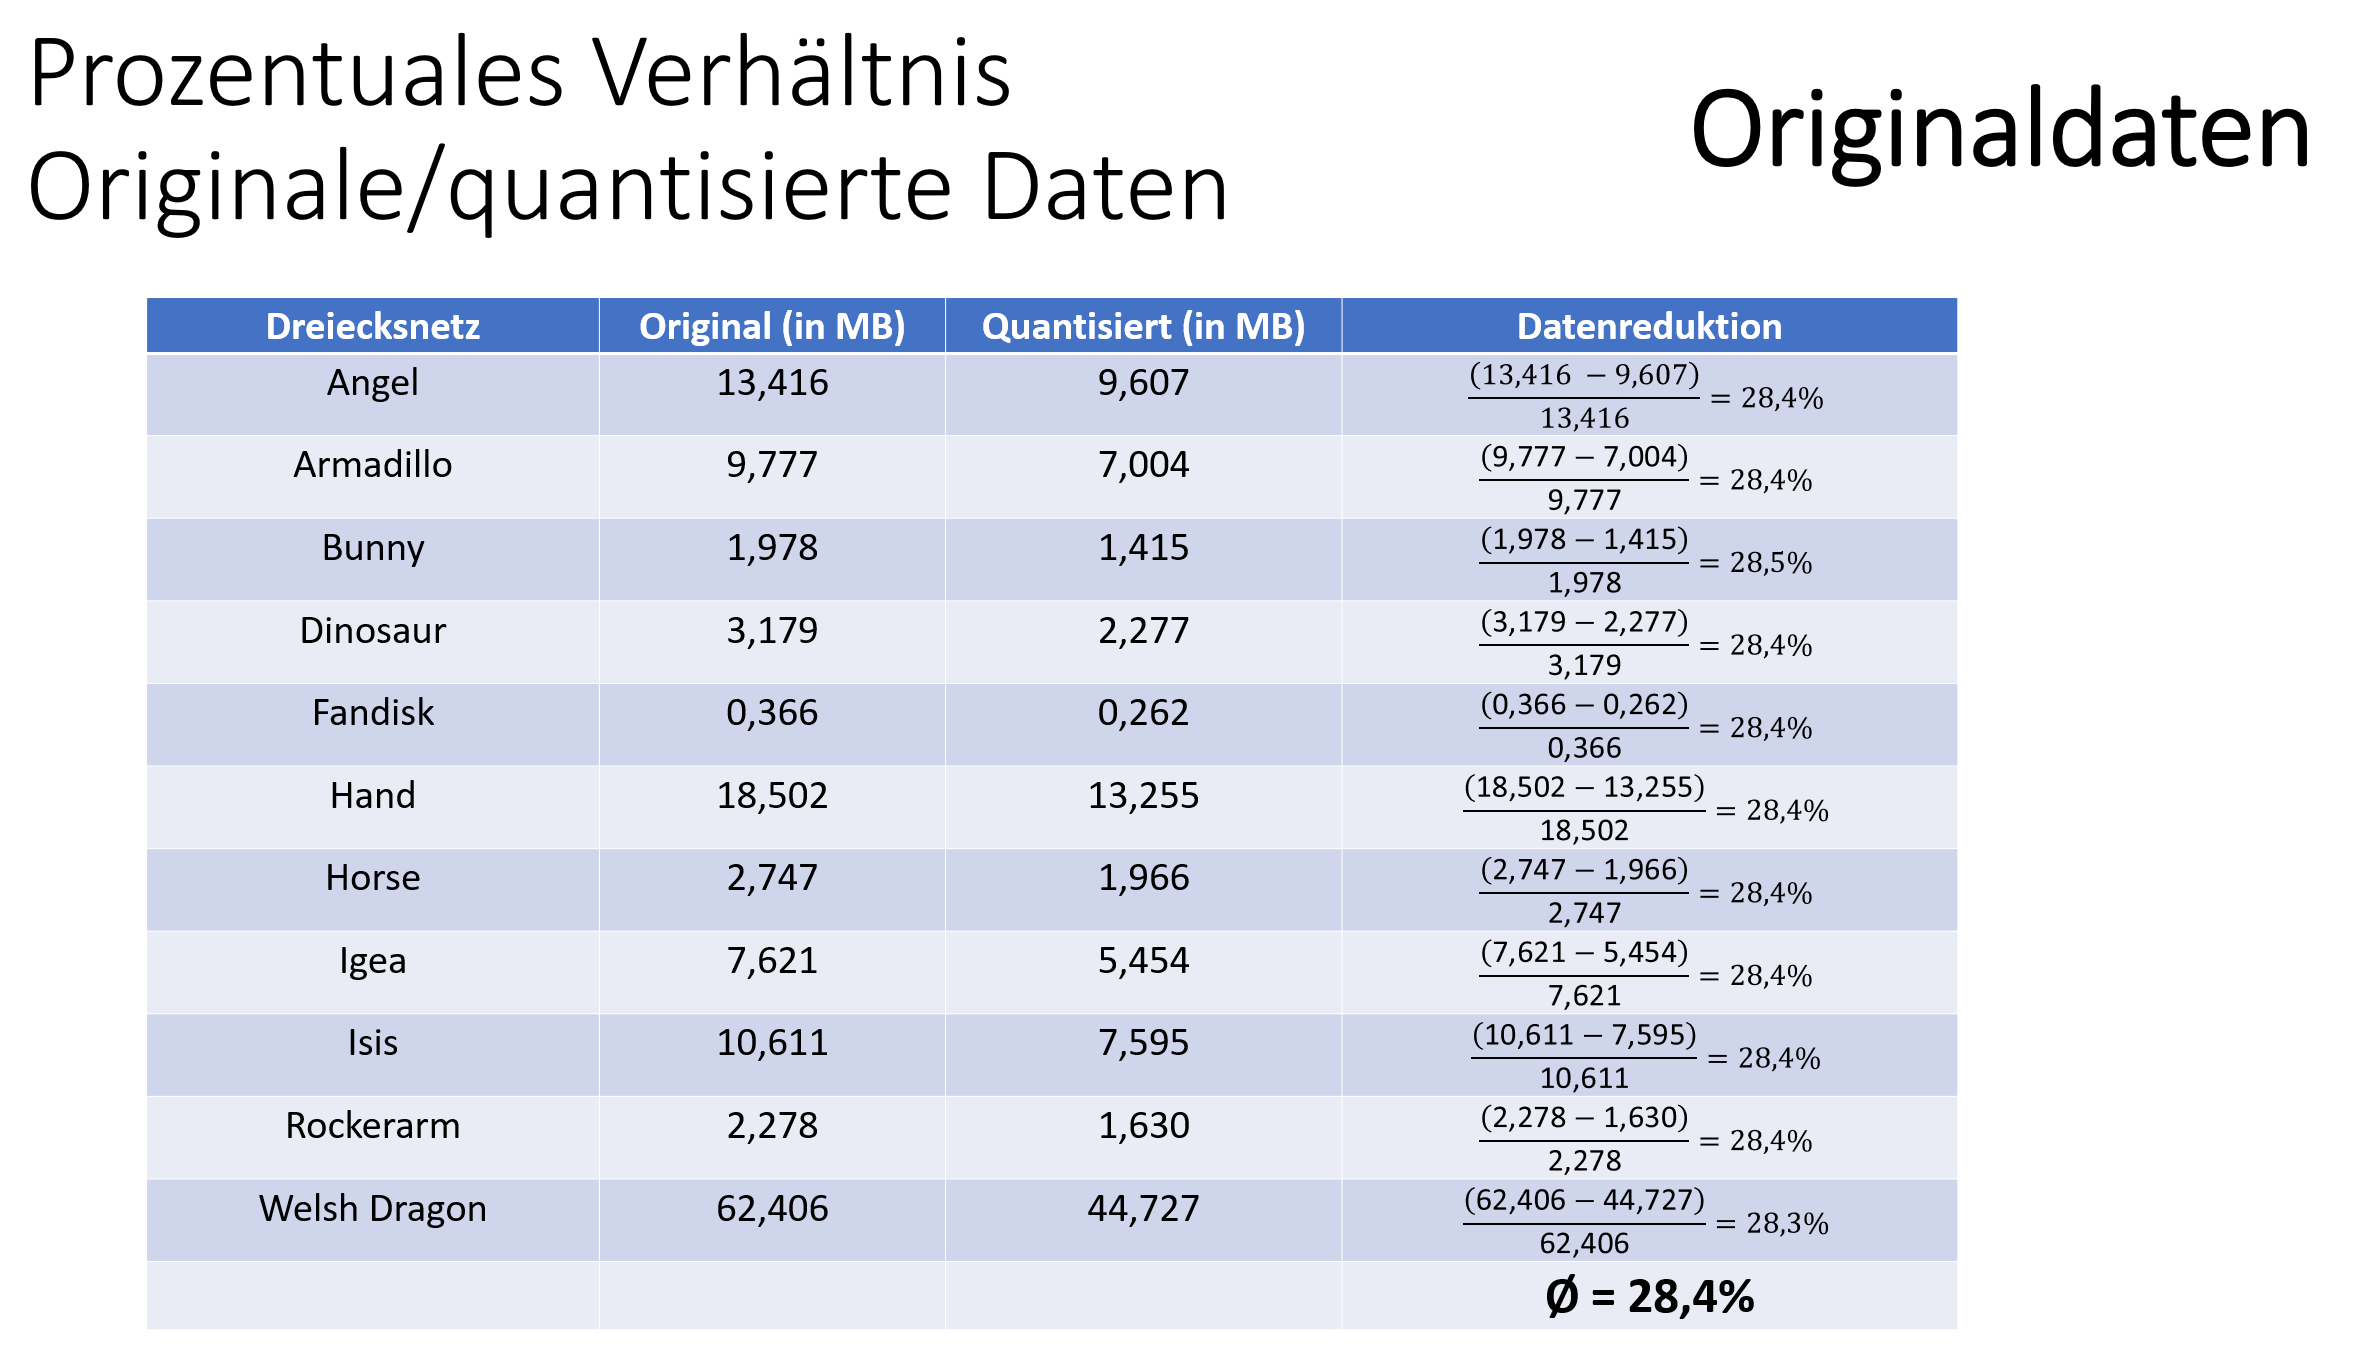
\includegraphics[scale=0.24]{Bilder/ergebnisse_full/orig_proz.png}
\end{figure}
\begin{figure}[h]
  \centering  
  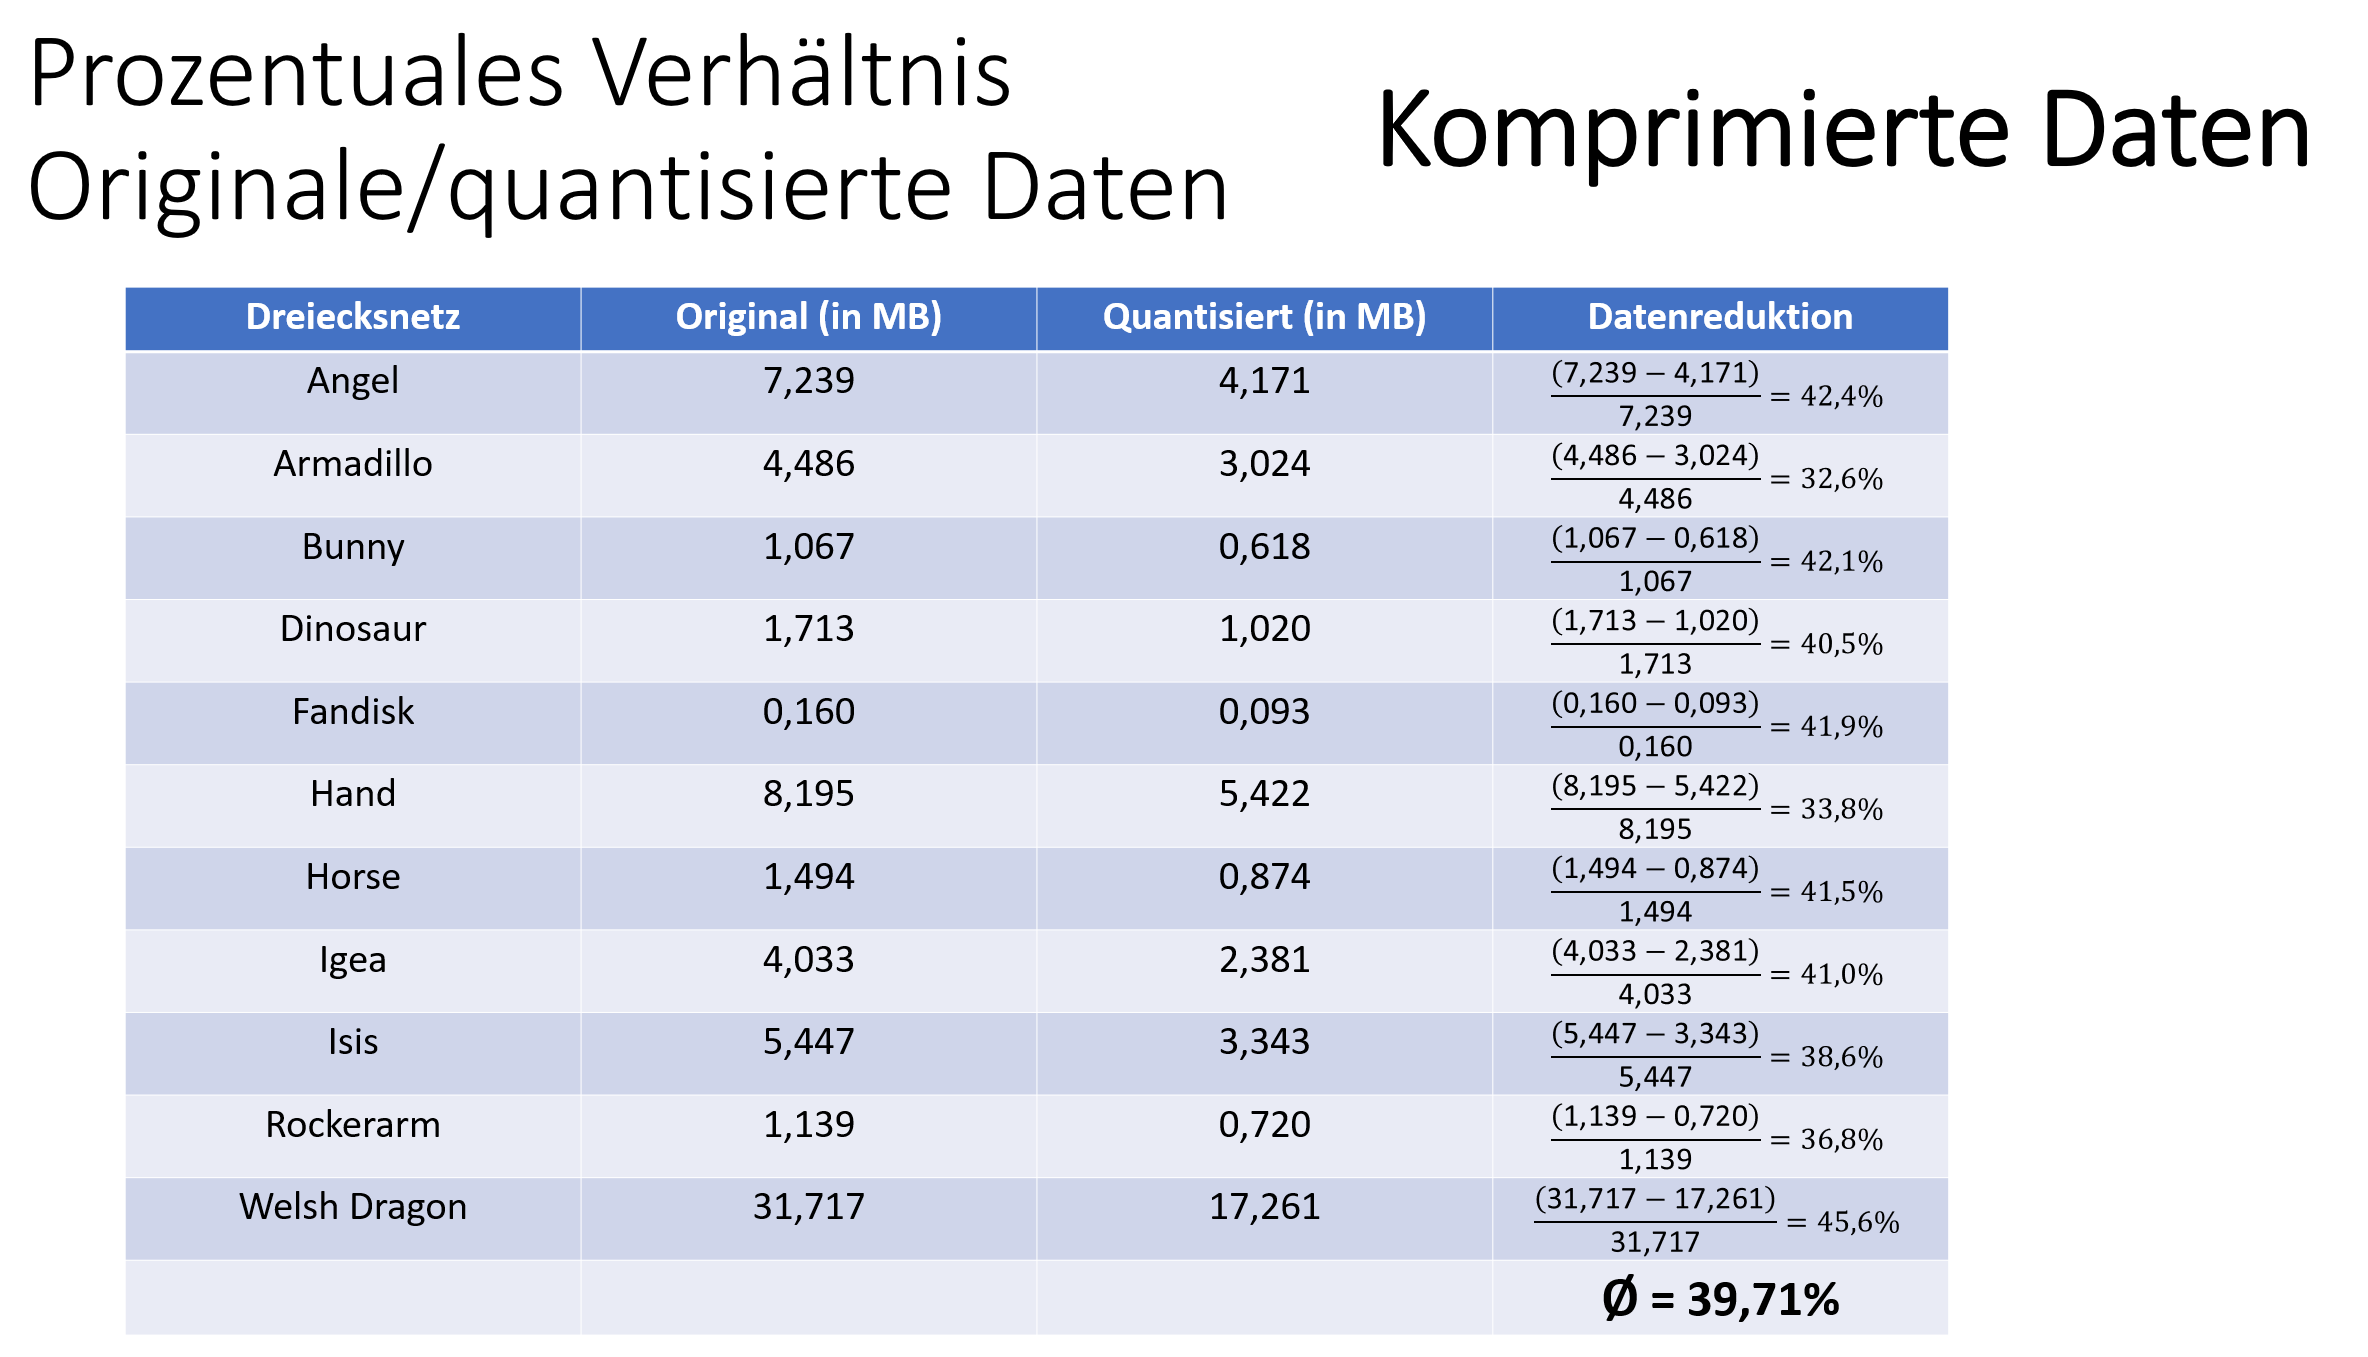
\includegraphics[scale=0.24]{Bilder/ergebnisse_full/komp_proz.png}
\end{figure}
  }{}

  % Declaration of Honor
  \newpage
  \phantomsection
  \addcontentsline{toc}{section}{Ehrenwörtliche Erklärung}
  \lhead{Ehrenwörtliche Erklärung}
  \pagestyle{plain}
\pagenumbering{gobble}


\textbf{{\Large Ehrenwörtliche Erklärung}}
\vspace{2cm}

% Determine article for document type
\ifthenelse{\equal{\DocumentType}{Praxisbericht}}
  {\newcommand{\DocumentArticle}{meinen}}
  {
    \ifthenelse{\equal{\DocumentType}{Bachelorarbeit}}
      {\newcommand{\DocumentArticle}{meine}}
      {
        \ifthenelse{\equal{\DocumentType}{Masterarbeit}}
          {\newcommand{\DocumentArticle}{meine}}
          {\newcommand{\DocumentArticle}{meine/n}}
      }
  }

Ich versichere hiermit, dass ich \DocumentArticle\ \DocumentType \ mit dem Titel
\vspace{1cm}

\begin{tabular*}{\linewidth}{@{\extracolsep{\fill}}ccc}
 \\ \hline
 \vspace{2cm}
 \\ \hline
\end{tabular*}
\vspace{2cm}

selbständig verfasst, keine anderen als die angegebenen Quellen und Hilfsmittel benutzt
sowie nicht an anderer Stelle als Prüfungsarbeit vorgelegt habe.
\vfill

\begin{table*}[hp]
  \centering
  \begin{tabular}{L{6cm}L{2cm}L{6cm}}
    & & \\
    & & \\ \cline{1-1}
    Ort &  \\
    & & \\
    & & \\
    & & \\
    & &  \\ \cline{1-1} \cline{3-3}
    Datum & & Unterschrift \\
  \end{tabular}
\end{table*}

  % TODO list
  \iftotalcounttodos
    \listoftodos[TODOs]
  \fi

  \end{document}
}

% ===========================================================================
%                   Simplified centered & colored tables
% ===========================================================================

\newenvironment{colortable}[1]{
  \begin{center}
    \begin{tabular}{#1}
    \hline
    \rowcolor{Gray}
}
{
    \hline
    \end{tabular}
  \end{center}
}

\newcommand{\tablecontent}{
  \hline
  \rowcolor{White}
}


\def\Studiengang{Informatik}
\def\Autorenname{Janek Foote}
\def\Dozent{Quirin Meyer}
\def\Titel{Geometriedekompression von Dreiecksnetzen auf der GPU}

% Infos zum Unternehmen
\def\Unternehmen{<FIRMENNAME>}
\def\Abteilung{<ABTEILUNG>}
\def\Strasse{<STRAßE>}
\def\Ort{<ORT>}

% Infos zum Betreuer
\def\Betreuer{Quirin Meyer}
\def\Funktion{<FUNKTION BETREUER>}
\def\Telefon{<TELEFONNUMMER BETREUER>}
\def\Email{<BETREUER EMAIL>}

% Daten
\def\Beginn{<BEGINN>}
\def\Ende{<ENDE>}
\def\Abgabe{13.03.2024}

\startHSCdocument[Bachelorarbeit]

  \section{Einführung}

In der Computergrafik ist die Erzeugung eines Dreiecksnetzes eine gängige Methode zur Generierung von 3D-Modellen. Diese Modelle können in Topologie und Geometrie unterteilt werden. Für die Geometrie werden verschiedene Attribute benötigt. 
So werden die Positionen, die Normalenvektoren und Texturekoordinaten/Farbwerte für jeden Punkt des Dreiecksnetzes in single-precision floating point values (32 Bit Gleitkommazahlen) gespeichert. 
Für die korrekte Annordung und Reihenfolge der Knotenpunkte ist die Topologie zuständig. 
Dabei ist die Datenkompression ein entscheidendes Thema. 
In einer Welt, in der digitale Daten schon lange ein wichtiges Thema sind, und dennoch immer weiter an Bedeutung gewinnen, ist die effiziente Speicherung und Übertragung ein wichtiger Gesichtspunkt.
3D Modelle werden so gut wie überall benötigt. 
Videospiele und Animationsserien wären ohne nicht vorstellbar. 
Architekten können ihre Ideen auch ohne Bleistift auf das Papier (oder den Bildschirm) bringen.
Künstler wollen Modelle erschaffen, die den Eindruck gewinnen wollen, realitätsgetreu zu sein. 
Die Folge davon ist, dass diese Modelle stetig komplexer werden, und somit ein größerer Speicheraufwand benötigt wird. 
Um dem entgegenzuwirken, werden Methoden verwendet, diese digitalen Informationen zu komprimieren. \newline

\subsection{Geschichtliche Ausarbeitung Thema Datenkompression}
\label{subsec:main_kompression}
Ursprünglich zur Repräsentation von Daten entwickelt, wurde der Morse Code zu einem der wichtigsten Werkzeuge für die Kommunikation des 19. Jahrhunderts. 
Bestehend aus zwei Grundbausteinen, einem kurzen und einem langen Signal, konnten einzelne Buchstaben kodiert werden. 
Erweitert man dieses Alphabet mit einem weiteren \glqq Symbol\grqq\, einer Pause, die zwischen einzelnen Signalsequenzen eingelegt wird, können ganze Sätze übermittelt werden. 
Das bekannteste Werkzeug für den Morse Code ist der Telegraf, mit dem diese Signale über weite Strecken übertragen werden konnten.
Die Erfindung des Morsecodes findet im 21. Jahrhundert nicht nur seinen Zweck in dramatischen Momenten des in Film und Fernsehens. 
Es war zeitgleich ein früher und großer Meilenstein und Wegbegleiter für die Kompression einer Datenquelle (in diesem Fall das Alphabet). 
Durch Untersuchungen einer großen Anzahl an Literatur kann eine Buchstabenhäufigkeit berechnet werden. 
Diese sagt aus, wie wahrscheinlich es ist, welcher Buchstabe in einem Text folgt, ohne den aktuellen Kontext, in Form von vorgehenden Buchstaben, zu betrachten.
Da die Wahrscheinlichkeit eines Zeichens abhängig vom Alphabet ist, sollten diese nicht übergreifend verwendet werden. 
So sind die Buchstaben \glqq E\grqq\ und \glqq T\grqq\ die Buchstaben des englischen Alphabets, welche die höchste Auftrittswahrscheinlichkeit besitzen, während sich im deutschen Alphabet der Buchstabe \glqq E\grqq\ von der Masse abhebt.
%Datenkompression problem ausführen: durch ein stop Signal geht eine wichtige Eigenschaft verloren (eventuell binär)
Der Morse Code hat gezeigt, welchen Nutzen die Kompression von Information beinhaltet.
Zu Kriegszeiten hat dieser eine effiziente und schnelle Übermittlung von Informationen ermöglicht.
Dadurch konnte in Krisenmomenten schnell reagiert werden, um so größeren Katastrophen frühzeitig abzuwenden, aber leider auch zu verursachen.

\subsubsection*{Der Ist-Stand}
Springen wir in die heutige Zeit sehen wir die Auswirkung von komprimierten Daten.
Die meisten Menschen denken an JPEGs und PNGs, wenn sie an digitale Bilder denken.
Bekanntere Videoformate sind MP4, AVI und FLV.
Bei all diesen Formaten handelt es sich um komprimierte Rohdaten.
Das Filesystem eines jeden relevanten Betriebssystems komprimiert beim Speichern von Daten diese automatisch.
Zusätzlich dazu besteht noch die Möglichkeit, seine Daten manuell zu komprimieren mithilfe von Programmen wie 7Zip, WinRar oder WinZip.
Datenkompression kann in so gut wie allen Bereichen angetroffen werden.
Und die Gründe dafür sind simpel.
Speicherplatz ist teuer, und das Ressourcenmanagement wird deutlich vereinfacht, wenn die benötigte Hardware minimiert wird.
Betrachten wir das Streamen von Daten auf dem Beispiel des größten Videostreaming Dienstes Youtube.
Laut Statistiken werden pro Minute hunderte Stunden an Videomaterial hochgeladen Tendenz steigend (Abb.~).
\begin{figure}[htb]
  \centering  
  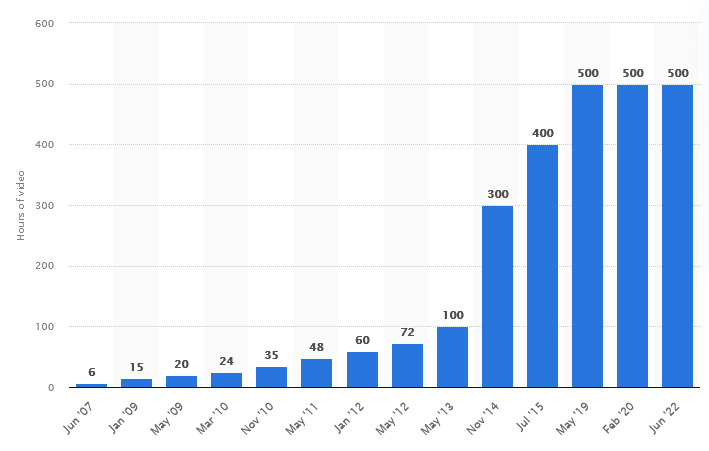
\includegraphics[scale=0.8]{Bilder/youtube_statistik.png}
  \caption[Youtube Statistik]{\textbf{Anzahl der Youtube Videos} Die Anzahl an Minuten die auf Youtube hochgeladen werden.
  Abbildung von Statista: https://www.statista.com/statistics/259477/hours-of-video-uploaded-to-youtube-every-minute/ }
  \label{fig:youtube}
\end{figure}
Um die Unmengen an Videos zu speichern, benötigt Google riesige Serverfarmen, die auf dem gesamten Globus verstreut sind.
Eine genaue Zahl ist der Öffentlichkeit nicht bekannt, es steht jedoch außer Frage, dass diese nochmal um einiges höher ausfällt, würde es keine Verfahren zur Datenkompression geben. \newline

Ein weiterer Gesichtspunkt ist der eigentliche Nutzen von Youtube, dem Streamen von Videos.
Um ein Video sehen zu können, muss dieses von dem Youtube Server, zum Nutzer, dem Client übertragen werden.
Durch die Komprimierung der Quelldateien sind die zu übertragenden Daten schon geschrumpft.
Es können jedoch noch weitere Schritte absolviert werden, um die Daten für den Nutzer besser zugänglich zu machen.
Dazu werden Verfahren wie Trancoding, Transsizing und Transrating verwendet.
Transcoding beschreibt den Prozess, ein bereits komprimiertes Videoformat in ein anderes, eventuell für den Client besser zugeschnittenes Videoformat zu komprimieren.
Das sollte jedoch nicht zu oft angewendet werden, da die Qualität beim wiederholten dekomprimieren und komprimieren verloren geht, sollten die Verfahren verlustbehaftet sein. \newline
In vielen Fällen kann die originale Auflösung vom Endgerät nicht abgespielt werden, und wird deshalb von diesem auf eine niedrigere Auflösung skaliert.
Beispielsweise wenn das Endgerät lediglich 1080p auflösen kann, aber ein Video in 4K Auflösung gestreamt werden soll.
Trotzdem werden die vollen Daten des Videoformats empfangen.
Um diese Verschwendung von Bandbreite zu sparen, wird Transsizing verwendet.
Die originalen Daten werden in eine kleinere Auflösung skaliert, und anschließend übertragen. \newline
Um die Bitrate zu minimieren wird Transrating verwendet.
So kann die Auflösung beibehalten werden bei jedoch geringere Bitrate.
Die Verfahren zur Minimierung des Datenstroms hören sich zunächst sehr mächtig an, sind jedoch mit Vorsicht zu genießen.
Der Vorgang ist nämlich Verlustbehaftet und kann bei zu starker Nutzung zu Artefakten führen.
Dafür ermöglicht es jedoch Menschen, deren Internetzugang ein Abspielen in hoher Qualität nicht zulässt, den Streaming Anbieter zu nutzen.

Der Ursprung der Datenkompression ist dementsprechend der Weiterentwicklung des Morse Codes zurückzuführen. 

TODO

\subsection{Steigende Komplexität}
\label{subsec:steigende_komplexität}
Um die Realität bestmöglich darzustellen, werden Modelle stetig detailreicher, wodurch die Anforderungen an der Hardware steigen. In einer komplexen Szene können mehrere Millionen Dreiecke sichtbar sein, die je nach Anwendung, in Echtzeit gerendert werden müssen. Der Wunsch nach realistischeren Modellen in der Animationsfilm und Videospielbranche hat die Dreiecksanzahl von 3D Modellen in die Höhe schießen lassen. 

\subsection{Ziel der Arbeit}

  \section{Grundlagen}

Obwohl Dreiecksnetze eine effektive Darstellung bieten, 3D-Modelle darzustellen, beanspruchen diese sehr viel Speicherplatz.
Mithilfe von Brotli-G sollen diese auf der CPU komprimiert, und auf der GPU dekomprimiert werden, sodass diese fertig zur Darstellung sind, ohne viel Bandbreite zu nutzen.
Damit der Weg von Komprimierung zu Darstellung verständlich ist, müssen einige grundlegende Dinge geklärt werden.

In diesem Grundlagenkapitel werden die von Brotli-G genutzen Algorithmen erläutert.
Zusätzlich wird ein Ausblick auf die Grafikpipeline gegeben, und die Stellen betrachtet, bei denen weitere Verbesserungen vorgenommen werden können.
Diese zeigt alle Transformationen, die die Daten eines Dreiecksnetzes von dem GPU Buffer bis zum Bildschirm durchläuft.

\subsection{Brotli Kompressionsstandard}
\label{subsec:brotli}
Brotli-G ist eine Weiterentwicklung des Brotli Kompressionsstand, der von AMD im Jahre 2022 entwickelt und veröffentlicht wurde.
Die AMD Spezifikation bietet parallele Datenverarbeiten nach dem SIMD Prinzip (Kap.~\ref{fig:simd_pattern}) auf Parallelrechnern, wie GPUs und Multithreaded CPUs.
Zum Verständnis des von AMD veröffentlichten Kompressionsmodells ist zunächst ein Blick auf das Original erforderlich. \newline

Brotli ist ein von Google Research entwickelter Kompressionsstandard, der 2013 veröffentlicht wurde.
Er ist darauf ausgelegt, Webinhalte effizienter zu komprimieren als ältere Standards wie Gzip oder Deflate.
BrotliG wurde mit bedacht auf Kompatibilität mit dem offiziellen Brotli entwickelt.
So sollte Brotli auch in der Lage sein, Inhalte, die mit BrotliG komprimiert wurden, zu entschlüsseln.
Zu beachten ist, dass dies nur in diese Richtung funktioniert, und somit Brotli das BrotliG Format nicht dekodieren kann  \cite{BrotliG2022}.

Brotli verwendet eine Kombination vieler Kompressionsalgorithmen, um Inhalte effizient zu komprimieren. 
Brotli's Kern besteht aus einem LZ77 Algorithmus, der in unterschiedlichen Ausführung auch in anderen Kompressionsstandard verwendet wird.
Der LZ77 Algorithmus wird zusätzlich mittels Huffman Codierung optimiert.

\subsection{Parallele Datenverarbeitung}
\label{subsec:flynn}
Michael Flynn unterteilte Rechnerarchitekturen in Kategorien, die Abhängig von der Anzahl der Instruktions- und Datenströme sind. \newline
Die Instruktions- und Datenströme:
\begin{enumerate}
\item[\textit{SI}] (\textbf{S}ingle \textbf{I}nstruction)
\item[\textit{MI}] (\textbf{M}ultiple \textbf{I}nstruction) 
\item[\textit{SD}] (\textbf{S}ingle \textbf{D}ata) 
\item[\textit{MD}] (\textbf{M}ultiple \textbf{D}ata) 
\end{enumerate}
können kombiniert werden. \newline

Dadurch ergeben sich die vier Rechnerarchitekturen \textit{SISD}, \textit{SIMD}, \textit{MISD}, \textit{MIMD}.
\subsubsection*{SISD (Single Instruction, Single Data)}
Die am häufigsten anzutreffene Rechnerarchitektur.
Bekannter unter den Namen Von-Neumann Architektur bearbeitet diese Architektur die auf dem Speicher befindlichen Daten seriell.
Man redet auch von skalaren Operationen auf die Daten.
Rechnerarchitekturen mit SISD sind leicht zu verstehen und die Verarbeitung ist vorhersehbar.
Der Preis dafür ist jedoch die langsame Geschwindigkeit gegenüber parallelen Architekturen.
\subsubsection*{SIMD (Single Instruction, Multiple Data)}
Um die Geschwindigkeit zu erhöhen, werden Daten, auf denen die selbe Operation ausgeübt wird, parallel verarbeitet.
Das ist bei der Berechnung von Vektoren und Matrizen von Vorteil.
Betrachten wir die Addition zweier Vektoren, so kann der resultierende Vektor berechnet werden, wenn die einzelnen Komponenten der Vektoren addiert werden (siehe Abb.~\ref{fig:simd_pattern}). Der Vertex Shader macht von dieser diesem Konzept Gebrauch, während dieser seine per-Vertex Operationen ausführt \cite{DalCin1996}.
\begin{figure}[htb]
  \centering  
  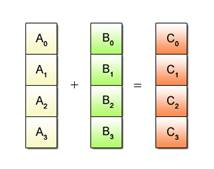
\includegraphics[scale=1.0]{Bilder/Simd_pattern.jpg}
  \caption[SIMD Pattern]{\textbf{Parallele Addition von Daten} In der Abbildung ist eine Addition verschiedener Daten zu sehen. Da die selbe Operation ausgeübt wird können die einzelnen Komponenten parallel verarbeitet werden.
  Abbildung ist aus http://ftp.cvut.cz/kernel/people/geoff/cell/ps3-linux-docs/CellProgrammingTutorial/BasicsOfSIMDProgramming.html }
  \label{fig:simd_pattern}
\end{figure} 
\subsubsection*{MISD (Multiple Instruction, Single Data)}
Um alle Kombinationen von Daten und Instruktionsströmen zu zeigen wurde auch MISD definiert.
Die Rechnerarchitektur bezieht sich darauf, das auf nur einem Datenpunkt verschiedene Operationen ausgeführt werden.
Für eine lange Zeit war diese Art von Rechnerarchitektur rein theoretisch anzutreffen, da weder 
\subsubsection*{MIMD (Multiple Instruction, Multiple Data)}
Wie auch die SIMD Architektur ist MIMD in Parallelrechnern anzutreffen.
Das Operationsprinzip von MIMD ist die Datenparallelität.
Das Funktionsprinzip von MIMD-Rechnern umfasst die gleichzeitige Ausführung von Anweisungen durch mehrere Prozessoren, die entweder über gemeinsame Variablen oder durch Nachrichten miteinander kommunizieren \cite{DalCin1996}.
TODO später \cite{Jakob2017} \newpage

\subsection{Die traditionelle Rendering Pipeline}
\label{subsec:traditionelle_renderingpipeline}
Um den Nutzen der neu vorgestellten Task- und Mesh-Shader Pipeline zu verstehen, muss zunächst die traditionelle Pipeline dort betrachtet werden, wo sie verbessert werden kann.
Die Rendering Pipeline besteht aus eine Reihe von programmierbaren (Abb.~\ref{fig:traditional_pipeline} grün dargestellt) und fixed-function (Abb.~\ref{fig:traditional_pipeline} türkis dargestellt) Stages.
Dazu kommt, das einige dieser Stages optional sind.
\begin{figure}[htb]
  \centering  
  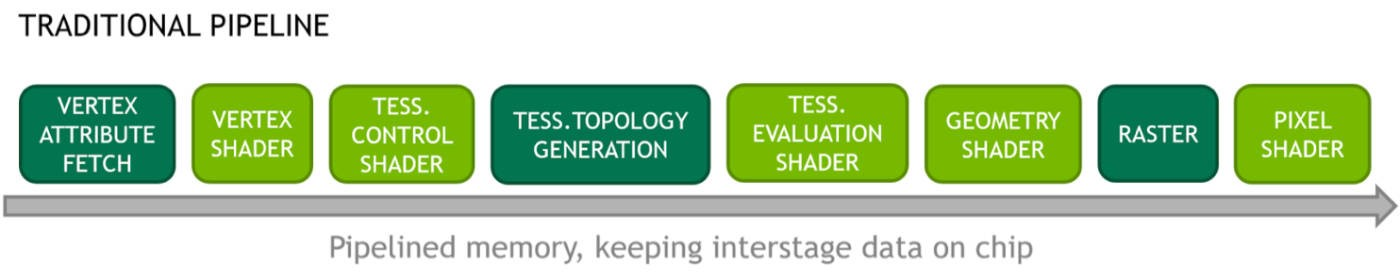
\includegraphics[scale=0.43]{Bilder/traditionelle_pipeline.jpg}
  \caption[traditionelle Rendering Pipeline]{\textbf{traditionelle Rendering Pipeline} \newline Die Abbildung beschreibt den Verlauf durch die einzelnen Shader Stages, die jeder Vertex macht. Entnommen wurde diese aus dem NVidia Blogpost \cite{Kubisch2018}}
  \label{fig:traditional_pipeline}
\end{figure}
\newline
Im GPU Memory angekommen, liest die \textit{Vertex Attribute Fetch} Stage die Vertex Daten aus, und sendet diese an den Vertex Shader.
Die Vertex Daten werden dort in die benötigten Koordinatensysteme transformiert und der optionalen Tessellation Stage weitergegeben, falls diese verwendet wird.
Die Tessellation Stage ist dazu da, Patches von Primitiven in kleinere Primitiven zu unterteilen.
Der optionale Geometry Shader kann dazu verwendet werden, weitere Vertices zu generieren.
Im Rasterizer angekommen, werden Primitiven verarbeitet und daraus Fragmente berechnet, denen der Fragment Shader zum Abschluss ihre Farbe gibt. \newline
Im Folgenden werden die einzelnen Stages nochmal genauer erläutert.

\subsubsection{Vertex Shader}
\label{subsubsec:vertex}
Zunächst wird der vom Entwickler programmierbare Vertex Shader angesteuert.
Dieser ist nicht optional, da alles nachfolgende auf den ausgegebenen Vertices aufbaut.
Hier können Operationen auf einzelnen Vertices ausgeführt werden.
Dafür wird der Vertex Shader für jeden Vertex einzeln aufgerufen.
Hier zeichnet sich das SIMD Modell der GPU aus (Kap~\ref{subsec:flynn}), da der Vertex Shader von mehreren Prozessoren auf unterschiedlichen Vertices zeitgleich operiert.
Die Inputs des Vertex Shaders werden mittels \textit{Vertex Attribute Locations} in den Shader eingebunden.
Der Shader kann dadurch die Positionen, Normalen und Texturkoordinaten von der CPU aufnehmen.
Eine Einschränkung, die dabei aufkommt, ist das Verhältnis von Eingabe und Ausgabe Vertices.
Der Shader erwartet, dass für jeden Eingabe Vertex auch ein Vertex ausgegeben wird.
Die Vertex Position wird für gewöhnlich in den Clip-Space transformiert, und der Pipeline weitergegeben.

\subsubsection{Tessellation Stage}
\label{subsubsec:tesselation}
Die Ausgabe Vertices des Vertex Shaders gelangen anschließend in die optionale Tessellation Stage.
Der generelle use-case ist, einen Patch an Primitiven in wiederum kleinere Primitiven zu verarbeiten. 
Die Tessellation Stage wird in drei Schritte unterteilt.
Darunter ist mit dem \textit{Tessellation Control Shader} (TCS) ein optional programmierbarer Schritt, eine fixed-function mit der \textit{Primitive Generation} und einen programmierbaren \textit{Tessellation Evaluation Shader} (TES).

\subsubsection*{Tessellation Control Shader (TCS)}
Der \textit{Tessellation Control Shader (TCS)} (der wiederum optional ist), ist ein geeigneter Schritt um das \textit{LOD} (Level of Detail) zu berechnen und unter gewissen Voraussetzungen vorab einige Patches zu cullen. 
Ein Patch beschreibt eine Anzahl an Primitiven.
Aus der Subdivision dieses Patches werden weitere Vertices berechnet, die zur Verarbeitung in den nächsten Schritt der Pipeline geschickt werden.
Im TCS wird der Grad der Tessellation, das Spacing zwischen subdivided Punkten und die gewünschte Topologie festgelegt.
Genauer gesagt wird hier gesetzt, wie oft die Primitiven unterteilt werden und welche Form diese am Ende haben sollen (triangle, quad, isolines).

\subsubsection*{Tessellation Topology Generation (TPG)}
Mit der fixed-function stage des Tessellation Schritts werden die Primitiven mittels den im TCS bestimmten Parametern unterteilt.
Die Koordinaten werden anschließend für den Tessellation Evaluation Shader berechnet.
Diese unterteilt die Patches abhängig von den Berechnungen der TCS.

\subsubsection*{Tessellation Evaluation Shader (TES)}
Der \textit{Tessellation Evaluation Shader} hat den einfachsten Job und realisiert lediglich die Arbeit, die von den zwei vorherigen Stages verrichtet wurde.
Die berechneten Koordinaten des TPG werden in dieser Shader Stage interpoliert, um die neuen Vertices zu generieren.
Abschließend werden die aus der Subdivision berechneten Vertices ausgegeben. 
Wenn der optionale TCS nicht genutzt wird, werden default Parameter für den TPG benutzt. \cite{cozzi2012opengl}\cite{Carvalho2022}

\subsubsection{Geometry Shader}
\label{subsubsec:geometry_shader}
Ein weiterer optionaler Schritt in der traditionellen Grafikpipeline ist der \textit{Geometry Shader}.
Er bekommt eine Primitive als Input, und kann keine oder auch mehr Primitiven ausgeben, als er bekommen hat.
Die Fähigkeit zusätzliche Vertices zu generieren ist auch das, was den Geometry Shader besonders macht.
Der Geometry Shader bekommt seinen Input entweder vom TES, oder, wenn die Tessellation Stage keine Verwendung findet, vom Vertex Shader und leitet seine Ausgabe an den Fragment Shader weiter.
Um Bandbreite zwischen CPU und GPU zu sparen, kann ein Geometry Shader ein Dreiecksnetz mit wenigen Dreiecken erweitern und dieses so detaillierter gestalten.
Ähnlich wie bei der Tessellation, die auf \textit{Patches} von Primitiven agiert, verarbeitet der Geometry Shader die Primitiven an sich.

\subsubsection{Pixel Shader}
\label{subsubsec:pixel_shader}
Der Pixel bzw. Fragment Shader ist der letzte programmierbare Schritt der Grafikpipeline.
In diesem werden die transformierten Vertices und Primitiven schlussendlich gezeichnet.
Der Pixel Shader operiert jedoch nicht auf diesen Daten, sondern auf sogenannten \textit{Fragmenten}.
Das bedeutet, bevor der Pixel Shader seinen Input bekommt, müssen Vertices und Primitiven erst durch den Rasterizer.
Nun liegt es am Entwickler, den einzelnen Fragmenten ihre Farbe zu geben.
In einem Modell werden per-Vertex Texturkoordinaten gesetzt, die auf eine Texturemap verweisen.
Im Fragment Shader wird diese Texturemap mittels Sampler interpoliert.
Zusätzlich müssen noch Materialeigenschaften beachtet werden.
Alternativ kann jeder Vertex auch seinen eigenen Farbwert besitzen. \newline

Um der Szene mehr Realismus beizusteuern, kann im Fragment Shader auch ein Lichtmodell implementiert werden.
Beispiele dafür sind \textit{Flat shading}, \textit{Gouraud shading} und \textit{Phong shading}.
Für die Lichtberechnung werden die Oberflächen-Normalen benötigt.
Diese sind entweder in einem Dreiecksnetz gegeben, oder müssen noch berechnet werden.
Ausgabe des Pixel Shaders ist wiederum ein Fragment.

\subsection{Compute Shader}
\label{subsec:compute_shader}
Der Compute Shader gehört nicht zur traditionellen Grafikpipeline, kann darin aber seinen Nutzen finden.
Sie dienen dazu, jede Mögliche Information die gewünscht ist auf der GPU zu berechnen.
Anders als bei den Shader Stages der traditionellen Grafikpipeline (Kap.~\ref{fig:traditional_pipeline}), erwartet der Compute Shader keine definierten Input/Output Daten, wie beispielsweise der Vertex Shader, der als Input und Output einen Vertex erwartet.
Der Compute Shader kann also willkürliche Daten verarbeiten und dabei noch die Parallelisierung der GPU nutzen \cite{Compute24}. \newline

Wie schon gesagt erhält der Compute Shader keine Input Variablen wie beispielsweise der Vertex Shader.
Im Gegensatz zu diesem werden benötigte Daten mittels Buffer und \glqq Shader Ressource Views\grqq\ auf die GPU geladen (in D3D12).
Aber ganz ohne Inputs kommt der Compute Shader nicht aus.
Vor Aufruf des Compute Shaders muss bestimmt werden, mit wie vielen Threads dieser arbeiten soll.
Der Aufruf der Dispatch Methode mittel Grafik API führt dazu, das der aktuell aktive Compute Shader aufgerufen wird.
Die Dispatch Methode nimmt die Anzahl an Threads in drei Dimensionen als Argument.

Dafür gelten jedoch Hardware Limitierungen.
Für die Anzahl der Threads muss gelten
\begin{gather*}
	numThreadsX, numThreads, numThreadsZ \leq 128 \\
	numThreadsX * numThreadsY * numThreadsZ = 1024
\end{gather*}
(Für Compute Shader Version 5\_0)

Um das SIMD Konzept des Compute Shaders zu verstehen sind zwei Variablen elementar wichtig.
SVGroupThreadID und SVGroupID.
TODO

\subsection{Grundbegriffe der Datenkompression}
\label{subsec:grundbegriffe_datenkompression}

Entscheidungsgehalt
Redundanz
Entropie

  \section{Task und Mesh Shader}
Die Architektur, auf der die neuartigen RTX-GPUs von Nvidia aufbauen, erweitert die Möglichkeiten, wie die Parallelisierung von GPUs genutzt werden kann.
Mit der GeForce RTX 20er Serie wurden die ersten GPUs mit der Turing Architektur veröffentlicht, die sich auch an Privatpersonen richtet.
Als großer Verkaufspunkt wurde bereits früh mit den Möglichkeiten von Real-time Raytracing und Deep Learning durch Tensor Core geworben \cite{Burgess2020}. 
Eine wesentliche Änderung an der Grafikpipeline wird jedoch bis heute noch relativ wenig Beachtung geschenkt.
Mit dem Shader Model 6 hat NVidia ihre sogenannte "next-generation shading Pipeline" vorgestellt.
Damit wird eine Alternative zur traditionellen Shading Pipeline gestellt, die dem Entwickler mehr Freiheit überlässt, die Parallelisierbarkeit der GPU zu nutzen.
Der Mesh Shader hat die Eigenschaften des Compute Shaders \ref{subsec:compute_shader}, der Daten auf der GPU parallel verarbeiten kann.
Auch Geometrie Daten können mithilfe des Compute Shaders berechnet werden, jedoch ist der Compute Shader kein Teil der traditionellen Grafikpipeline und findet dadurch seinen Nutzen auch außerhalb des Renderings \cite{Ilett2022}.
Mit der \textit{Mesh Shading Pipeline} wurde die Möglichkeit der Parallelisierung des Compute Shaders mit der neuen Rendering Pipeline verknüpft.
Anders als bei der herkömmlichen Grafikpipeline erhält der Mesh Shader seine Daten direkt vom Speicher. 
Dadurch öffnen sich Türen für den Entwickler, da er komprimierte Daten direkt in den GPU Speicher laden kann, um die Daten dann effizienter auf dieser zu dekomprimieren.


\subsection{Meshlets}
\label{subsec:meshlets}
Um die neuartigen Shader für das Rendering zu verwenden, wird empfohlen, das gesamte Mesh in kleinere Subsets, sogenannte Meshlets, zu unterteilen. 
Die traditionelle Grafikpipeline verarbeitet die Daten des Dreiecksnetzes in serieller Manier. 
Dadurch kommt es jedoch zu Bottlenecks.
In der traditionellen Pipeline werden Vertex und Primitiven zugeschnitten und in kleine Clustern verarbeitet.
Dazu wird der Primitive Distributor vor der Vertex Shader Stage aufgerufen.
Dieser liest die Daten des Index Buffers und generiert dementsprechend möglichst performant diese Cluster an Daten.
Der Schritt des Primitive Distributor ist jedoch eine fixed-function Stage der Grafikpipeline, wodurch der Entwickler keinen direkten Zugriff hat.
Das hat zur Folge, dass die Cluster nicht auf die Bedürfnisse des Entwicklers und dessen Implementierung angepasst werden können.
Zuzüglich werden die Cluster zu jedem Frame, bzw. vor jedem Aufruf der Pipeline neu generiert.
Dieser Schritt ist redundant, sollte das Dreiecksnetz zur Laufzeit unverändert bleiben \cite{Carvalho2022}, \cite{Kubisch2018}. \newline

Durch die Compute Shading Natur des Mesh Shaders ist der Input der Daten nicht mehr festgelegt wie bei der traditionellen Pipeline.
Dadurch kann der Entwickler seine eigenen Implementationen zur Generierung von Meshlets verwenden.
Anders als bei der herkömmlichen Grafikpipeline werden Meshlets auf CPU Ebene erstellt.
Dazu werden Vertex Positionen und Indizes benötigt.
Die Anzahl der Vertices und Primitiven muss im Vorfeld festgelegt werden.
Die Auswahl der Meshletgröße ist abhängig von der verwendeten GPU.
So wird im NVidia Blogpost \glqq Introduction to Turing Mesh Shaders\grqq\ eine maximale Anzahl an Vertices von 64, und Primitiven von 126 empfohlen. 
Es werden 126 statt 128 Primitiven empfohlen, da 4 Byte für die Anzahl der Primitiven verwendet werden, die im selben Block Speicher enthalten sein sollen, bzw. keinen weiteren Block beanspruchen sollen \cite{Kubisch2018}.
Arseny Kapoulkine hat verschiedene Meshletgrößen miteinander verglichen.
Er ist zu dem Schluss gekommen, dass 64 Vertices und 84 Primitives am effizientesten ist, insbesondere dann, wenn im Task Shader Culling an den einzelnen Meshlets betrieben wird.
Des weiteren ist die Empfehlung des Blogposts nach eigenen Tests zwar ein guter Maßstab, jedoch wird im Durchschnitt viel Speicher des Primitiven Buffers ungenutzt bleiben, da die 126 Primitiven mit 64 Vertices nie erreicht werden \cite{Kapoulkine2023}.

\subsection{Implementierung Mesh Shader}
\label{subsec:meshshaderimpl}
Wie im vorherigen Unterkapitel angekündigt muss das Dreiecksnetz auf der CPU zu Meshlets geschnitten werden. 
Dazu wurde in dieser Arbeit er Meshoptimizer von Zeux verwendet \cite{Zeux}. 
[Implementierung von Zeux beschreiben]
Die Funktion \glqq meshopt\_buildMeshlets\grqq\ nimmt als Eingabeparameter die maximale Anzahl an Vertices und Primitiven (Kap.\ref{subsec:meshlets}), die Vertex und Index Daten sowie drei leere Buffer.
Der Buffer \textit{meshlet\_indices} wird die neuen Index Daten enthalten, mit denen die Primitiven berechnet werden können.
Der \textit{meshlet\_vertices} Buffer beinhaltet die einzigartigen Vertices des Dreiecksnetzes (Kap~\ref{subsec:primitive_subgroups}).
Der letzte Buffer wird in dieser Arbeit als \textit{Meshlet Descriptor} bezeichnet.
Der Einfachheit halber wird er im Code jedoch einfach als \textit{meshlets} implementiert.
Der Meshlet Buffer setzt sich auch folgenden Elementen zusammen
\begin{itemize}
\item Vertex Count: Die Anzahl der Vertices V in dem Meshlet mit dem Index i
\item Primitive Count: Die Anzahl der Primitives P in dem Meshlet mit dem Index i
\item Vertex Offset: Die Menge an Schritten im Vertex Buffer, um an die Vertices des i-ten Meshlets zu gelangen
\item Primitive Offset: Die Menge an Schritten im Index Buffer um an die Primitives des i-ten Meshlets zu gelangen
\end{itemize}

Mit den Informationen der originalen Vertexdaten und der drei neu generierten Buffer \textit{meshlet\_indices}, \textit{meshlet\_vertices} und \textit{meshlets}, kann nun der Mesh Shader gefüttert werden.
Zunächst müssen die während des Build-Vorgangs kompilierten Shader gelesen werden.
Diese enthalten Informationen zum Layout der Root Signature, die daraufhin per API-Call erstellt wird.
Bevor die Meshlet Daten an den Mesh Shader übergeben werden können, müssen diese in einen GPU Buffer geschrieben werden, damit diese anschließend in den GPU RAM geschrieben werden können.
Wenn das alles gemacht ist können in der Commandlist der Constant Buffer und die benötigten Meshletdaten über die DirectX12 API-Calls SetGraphicsRootConstantBuffer und SetGraphicsRootShaderRessourceView gesetzt werden.

\subsection{Mesh Shader Implementation}
\label{subsec:mesh_shader_impl}
Im Codeabschnitt~\ref{lst:shadercode} ist ein einfacher Mesh Shader zu sehen.
Im Mesh Shader wird die Root Signature entsprechend den Anforderungen gesetzt.
Minimal wird ein StructuredBuffer für jeden der auf der CPU generierten Meshlet Buffer benötigt.
Um dem Endresultat 3-Dimensional wirken zu lassen, wird ein ConstantBuffer verwendet, der die\textit{model}, \textit{modelView} und \textit{modelViewProjection} Matrix beinhaltet. 
Zusätzlich dazu nimmt der Constant Buffer noch ein boolean, um zu steuern, das die Meshlets farbig hervorgehoben werden.
Zunächst wird das aktuelle Meshlet aus dem \textit{Meshlet Descriptor Buffer} genommen.
Die SV\_GroupID stellt in dieser Implementierung den aktuellen Index der Meshlets dar.
Um den lokalen Index des aktuellen Meshlets zu bekommen, muss die SV\_GroupThreadID verwendet werden.
Die aktuelle GroupID wird in einzelne Threads unterteilt, damit die GPU sich bei der parallelen Verarbeitung nicht in die queere kommt.
Die Anzahl der Threads wird mittles \textit{[NumThreads(128, 1, 1)]} im Mesh Shader, oder, falls vorhanden, im Task Shader festgelegt.

\newpage \begin{lstlisting}[language = C++, caption = Mesh Shader Main, label=lst:shadercode]
[RootSignature(ROOT_SIG)]
[NumThreads(128, 1, 1)]
[OutputTopology("triangle")]
void main(
    in uint gtid : SV_GroupThreadID,
    in uint gid : SV_GroupID,
    out vertices VertexOut verts[64],
    out indices uint3 tris[84]
)
{
  Meshlet m = Meshlets[gid];
  uint3 primitive;

  SetMeshOutputCounts(m.VertCount, m.PrimCount);
  
  if (gtid < m.PrimCount)
  {
    primitive = GetPrimitive(m, gtid);
    tris[gtid] = primitive;
  }
  
  if (gtid < m.VertCount)
  {
    uint vertexIndex = GetVertexIndex(m, primitive[0]);
    verts[gtid] = GetVertex(gid, vertexIndex);
  }
}
\end{lstlisting}

\subsection{Das auf der GPU zu dekodierende Binärformat}
\label{subsec:binary_format}
[Eventuell nicht als eigenes Unterkapitel]


\finishHSCdocument